\documentclass{LessonsFromJapan}

\usepackage{multirow}
\usepackage[figuresright]{rotating}

\begin{document}
    \pagenumbering{roman}
    \phantomsection
\thispagestyle{empty}
\vspace*{3em}
\begin{center}
  {\xbsong\zihao{-0}\xeCJKsetup{CJKglue=\hskip 2pt}以日为鉴：衰退时代\\生存指南\par}
  \vspace{4em}
  {\zihao{-3}\kaishu 分析师Boden\q 著\par}
\end{center}
\cleardoublepage
 \cleardoublepage
    \pagestyle{tocstyle}
    \pagenumbering{Roman}
    \tableofcontents
    \cleardoublepage
    \pagestyle{docstyle}
    \pagenumbering{arabic}

    % 来源：EPUB spine / EPUB/xhtml/chapter1.xhtml

\section[前言\q 关于《以日为鉴》]{前言\\ 关于《以日为鉴》}

笔者关于日本社会演变的案头研究工作，其实在十余年前就已经开始了，这些年更多的是将剖析日本作为一个研究爱好。2024年的一个意外契机，笔者将部分内容整理成文字与视频发布在网上，没想到收获了巨大的反响。经过半年的努力，笔者将这些年研究工作中认为精华的部分整理成册，形成了《以日为鉴》。

为什么要写这本《以日为鉴》？

其实关于日本泡沫破裂后的研究书籍，无论是日本作者的中译版，还是中国作者的研究内容，已经比较丰富了。但这些书籍更多都聚焦在一个宏观的叙事与国家层面的故事，哪怕有的涉及日本内阁与大藏省在这40年中做出的种种改革，也很少探究这些政策究竟会对一个个鲜活的个体产生哪些影响，更鲜少提及这些决定将对不同职业，乃至年龄群体产生哪些影响。

但笔者认为研究在失落经济之下，日本不同行业、职业与微观个体之间的相互影响其实更有意义。作为东亚第一个从“增长型社会”走向“存量型社会”的经济体，日本在这40年中走过了一轮完整的经济周期，而这40年中的变化其实就是一本“人生参考书”，或者说是“职业错题本”。

长达十余年的“就业冰河期”与房价暴跌后的债务危机，究竟会给个体带来怎样的伤害，不同的人生抉择会有怎样的后果，早已写到了日本社会发展的历史中。而这也是笔者撰写这本书的初衷，希望能够对这些经验与教训进行系统性的回顾，抛开宏大的叙事背景，站在普通人的角度去探寻这轮长达40年经济周期的借鉴意义。

其实地产泡沫经济崩裂后，日本先于东亚所有经济体经历了种种困境。无论是经济上的长期不景气与失业潮对社会意识形态的冲击，还是少子化与老龄化对不同群体与行业造成的压力，何尝不是东亚经济体在发展过程中的一个必经阶段。作为传统的儒家东亚文化圈的一员，日本社会在此经济下行期出现了诸如“返乡潮”“考公热”“学历贬值”“高学历贫穷”“医疗崩坏”“临时工时代”等社会现象，也诞生了“啃老族”“无缘社会”“老后破产”“女性贫穷”等社会名词。这些现象无一例外也在后来的韩国社会中出现。因此当周期的轮回指向我们时，研究这些现象形成的原因及其最终演变，对今天的我们极具现实意义和借鉴价值。

《以日为鉴》这本书将分为5个章节，在文章叙事上将从社会失业潮、大学生毕业潮、财政紧缩危机、老龄化与少子化，社会内卷与全民出海五个维度，去讲述不同群体的决策与境遇。笔者希望以这5个维度，带领读者去了解长期困扰日本的种种社会问题的根源。

第一章：我们将讲述在社会性失业潮下，当时日本政府在新员工与老员工，保就业与保发展，大都市与返乡之间的抉择，去理解不同的决策带给不同群体的具体影响，探索如今日本格差社会与地方不振现象形成的原因。

第二章：将以失落的一代人为视角，讲述泡沫破裂后毕业大学生们的境遇。也就是日本20世纪70年代第二次婴儿潮期间出生的近2000万人，他们如何从出生过剩走到毕业过剩，最后是就业过剩。看看延时毕业、教育市场化、硕博大扩招与派遣制度等改革在他们身上留下了什么痕迹。

第三章：将以就业为视角，回顾日本曾经的考公热与教师热。日本的“医师公”职业曾经以稳定与高收入被称为神的职业。在泡沫破裂后出现了全民考公潮，把公务员当作经济不景气的职业避风港，成为当时很多日本人的选择。但这轮热潮却只持续了10年。日本的考公热是如何燃起又落下的，公务员又如何成为如今日本学生最不愿意从事的职业？

第四章：将以老龄化社会的医疗体系为视角。20世纪80年代日本医疗产业一度俯视全球，但在90年代老龄化与财政紧缩的冲击下，却造就了“医疗崩坏”与“医药寒冬”两个社会热词。那么这场老龄化到底给医疗与医药产业留下了哪些伤痕，拯救日本医疗的再生改革与药品复兴改革到底是什么？

第五章：将以全民出海潮为视角。眼下中国市场内卷已经成为一个共识，越来越多的人开始关注出海的机会。日本泡沫经济结束后的90年代，出现过一轮长达20年的全民出海潮，成为失落经济下少数黄金赛道。当我们把日本90年代的视角从日本国内转换为国外，又会给今天的我们在未来职业选择上带来哪些借鉴？

笔者希望通过讲述日本社会、行业与职业的种种动荡，从其经验与教训当中找到一些共同的规律，好让后来者少走一些弯路。

最后，笔者还是想引用罗曼·罗兰的一句名言作为结尾：“世界上只有一种英雄主义，就是看清生活的真相之后依然热爱它。”而这也是《以日为鉴》这本书希望能够带给读者的价值，希望能够帮助读者在时代的巨大不确定性中，找到人生的确定性，并耐心地、坚定地，做好那些难且正确的事。

{\kaishu\hfill 分析师Boden\par}

{\kaishu\hfill 写于2025年春\par}
 \cleardoublepage
    % 来源：EPUB spine / EPUB/xhtml/chapter2.xhtml

\BookPart{第一篇}{失业潮下的决策}

\BookPartImage{image/第一篇失业潮下的决策.jpg}
 \cleardoublepage
    % 来源：EPUB spine / EPUB/xhtml/chapter2_0001.xhtml

\BookChapter{1}

\section[第一章\q 保就业，还是保发展？]{第一章\\ 保就业，还是保发展？}

\BookSubtitle{——回顾日本保就业史：为保就业付出了怎样的代价？}

{\fangsong 日本作为一个高度重视社会稳定的国家，在泡沫经济破裂后的经济下行期间，采用了众多手段将失业率长期压制在5\%以下，艰难地挺过了一轮轮失业潮，但有人认为，日本保就业的成果，是建立在牺牲长期发展与一代人的利益的基础上所取得的。\par}

{\fangsong 那么这一切是如何发生的？\par}

就业的稳定，是每一个社会群体最关心的话题。当经济下行时，经济增长的停滞往往会触发群体性失业问题。然而，在日本泡沫经济破裂后的10年经济下行期间，失业率却几乎始终控制在5\%以下。即便2001年至2003年那段经济最为艰难的时期，整个社会同时遭受互联网泡沫破裂、亚洲金融危机余波以及银行业破产潮的三重冲击，国民失业率也仅短暂上升至5.4\%。在20世纪90年代初泡沫经济瞬间破裂、房地产市场暴跌的悲剧下，日本社会并未出现严重的群体性问题，其保就业措施可谓功不可没。

但日本在保就业过程中付出的代价却极为沉重，甚至可以说是以牺牲一代人的利益为代价。本篇作为“以日为鉴”系列的第一篇，让我们从大众最关心的就业话题出发，回顾那段历史。

\subsection{一、经济只是短暂的失速}

如今我们已清楚地看到，日本的那轮经济衰退持续了近20年。但在90年代初，对于那个昨天还在全民高呼“日本可以说不”的社会来说，尽管衡量经济景气的CI指数\footnote{“CI指数”即“景气动向综合指数”（Composite Index），是日本政府用于衡量经济周期波动的重要指标之一。该指数由日本内阁府编制，分为一致指数（Coincident Index）、先行指数（Leading Index）和滞后指数（Lagging Index）三部分，分别反映当前经济状况、未来经济趋势及历史经济表现。}在1989年达到历史最高点114后便开始下滑，到1991年已跌破100，但所有人都认为这只是一次短暂的调整。1990年底，无数日本媒体热炒一个词——“未实现的收益”。政府和民众都坚信未来的股价还会继续上涨，目前的下跌只是暂时的，损失的只是尚未实现的收益，未来仍可重新获得。

对于企业而言，头脑发热的企业家们仍在加大产能投资。全行业设备投资额从1989年的54万亿日元增加到1991年的64万亿日元，而当年职工薪酬大涨5.6\%创下自1985年以来的最高水平。几乎所有人都笃信，这只是短暂的调整，经济复苏即将开始，于是纷纷加仓抄底。

但事实真的如此吗？1990年全国家用车销售数量达到510万台，相当于每20个日本人就有一个在当年置换新车，而到了1993年这一数字已经跌到400万台。而家用车这类家庭大宗消费往往代表了社会民众的信心，毕竟是否换车往往取决于未来几年的收入水平。可以说1990年这轮最后的疯狂，让无数民众与企业都抄底在最高点。而投资决策与经济周期的严重背离，也为后来180度的政策转向种下了苦果。

\subsection{二、泡沫破裂的惊醒}

1993年，日本迎来了就业危机的第一年。随着泡沫经济的余温消退，国民GDP迎来了自1974年以来的首次负增长，许多还沉浸在泡沫繁荣中的日本人瞬间清醒。然而比GDP负增长更糟糕的是失业率的快速增长。当年厚生省统计的全行业失业率从不足2\%跳涨至3\%，全国破产企业已经连续两年突破1万家。

而这场失业风暴也着实惊吓到了日本社会，长期的繁荣早已让很多人忘记了经济衰退的恐怖，甚至从未经历过失业的恐惧。自1975年石油危机后，日本一直处于高速增长状态，80年代更是成为全球少有的低失业率与高增长国家。在泡沫经济最疯狂的1985年至1989年，每年数千家企业因人手不足而破产，当时的公司招聘甚至需要预留一笔“接待经费”，用于招待前来应聘者的交通和餐食费用。1988年《朝日新闻》统计，东京地区面试者的平均交通费超过2000日元，而面试后如安排用餐，则标准至少为10000日元/位。否则，企业会被视为“失礼”，因为人们愿意来面试本身就是给了企业面子。

在这种大好形势下，整整一代人都没有接触过“失业危机”这个词，因为过去的20年告诉他们，工作总是唾手可得。

然而，随着泡沫经济的破灭，这种繁荣景象戛然而止。1993年厚生省的劳动经济报告开篇便是“失业动向：各行业岗位需求持续锐减”。而在两年前报告书首要讨论的问题还是“在经济景气扩大背景下：劳动力短缺与企业应对措施”。由此，日本政府开始了为期十余年的就业率保卫战，而这段时间就是在这本书里会被反复提起的“就业冰河期”。

\subsection{三、日本如何保住就业}

在深入探讨日本如何保住就业之前，我们有必要先了解一下当时企业所面临的困境。当时的日本企业遇上的最大问题便是企业利润快速下滑，但产能端却出现了严重的过剩，这使得企业陷入了恶性内卷和亏损的泥潭。根据日本大藏省统计，仅1993年全行业利润就同比下降了21\%，但全社会产能却出现了接近15\%的增长。

造成这一现象的主要原因，是由于大多数企业在1993年以前错误地评估了经济形势，误以为这只是一轮短暂的经济调整。因此，他们选择简单粗暴地增加产能，希望借此抢占市场，最终导致了产能的严重过剩。以日本水泥产业为例，本应该作为受房地产市场下行影响最大的行业，在地产泡沫破裂全国地价断崖式下跌的背景下，全行业却在三年内逆势增加了1000多万吨的产能。而当时面临相同问题的，又何止水泥这一个行业呢？

但不同于欧美资本主义企业在企业利润下滑与产能过剩时就裁员，日本企业基本遵循终身雇佣制度，员工愿意与企业共渡难关，企业自然也不能随意裁员。由此，日本政府陷入了保就业还是保发展的两难选择。如果放任这些利润下滑与产能过剩企业倒闭，固然能够实现过剩产能的出清，但也将引发巨大的社会性失业问题，这严重违背了日本传统的社会价值观。

在泡沫时期的终身雇佣制度下，企业被视为一个大家庭，员工需要尽忠尽职，但企业也不能抛弃每一个员工。而这也是日本为何有“窗边族”\footnote{“窗边族”，又称“内部失业”，指日本企业为了让高龄的普通员工或不适任的员工不干扰其他员工的工作，而将其安排在窗边的位置，不为其安排工作或是只安排杂务。部分企业为了节省遣散费，甚至将“窗边族”的办公用品撤下，逼迫其主动辞职。}文化的原因，哪怕这些大龄员工已经无法做出贡献，但他们依然是企业不能放弃的一分子。再加上，日本企业长期采用交叉持股、互相绑定的做法，上下游企业之间往往是共生关系，而非对立关系。即使个别企业出现破产，它们也很快会被关联企业收编，最大限度地保证了整个社会的稳定。这也是为何80年代日本员工也常常被称为企业战士的原因，因为企业就是他们的第二个家。

由于社会价值观很难接受企业倒闭与员工失业，迫于社会舆论压力，日本政府最终选择了一切为就业稳定让路。

在具体做法上，日本采用了企业改革与雇佣改革两大政策来稳定就业市场。

第一，企业改革。在企业改革方面，1994年开始日本政府的核心目标就是尽可能地不让企业破产。在具体运作上，采用了“大吃小”与“集群合并”两种思路，将行业内亏损企业与盈利企业进行合并，同时银行向大型企业提供贷款保证他们收购足够多的小企业，或者通过政府牵线让多家小企业集群合并抱团取暖。

第二，雇佣改革。在雇佣制度上，政府鼓励企业更多采用合同制雇员而非终身雇佣制的正式员工，同时出台了《劳务派遣法》采用“老人老办法新人新办法”的形式，逐步降低整个社会正式员工的数量，大幅度增加临时性员工数量。简单来说就是基本放弃了对大学生的培养，转而全力稳定对于已有工作经验群体的保障。

在这样强力的行政干预手段下，最终经过数年的调整，日本过剩产能基本被消化。还是以水泥行业为例。经过1993年到1997年大规模的兼并重组，到1998年，日本水泥行业整合为12个水泥集团，行业集中度大幅提高，相对稳定的格局基本形成。而到了2000年以后，随着日本的产业结构发生巨大改变，服务业成为日本主要的GDP贡献来源，而原有重工业和重化工业所占的比例大幅下降。整个社会岗位供给重新复苏。

最终经过10年的努力，日本失业率在2003年以后逐年下滑。全社会成功将日本在“就业冰河期”的失业率压制在5\%以下。社会普遍认为，到2003年日本基本已经走出了“就业冰河期”。

那么这样做，真的没有代价吗？

\subsection{四、保就业的代价}

后来有人总结，日本保就业的成果，是建立在牺牲长期发展与一代人利益的基础上所取得的。

我们先说说日本是如何牺牲发展来保就业的。其实经济过热之后的企业破产潮，本就是经济周期的必然阶段。但是为了保住就业，日本政府采取了一系列措施来避免企业破产和产能出清。这种做法虽然在短期内保住了就业，但却给日本经济发展留下难以愈合的伤口。

由于日本政府不顾企业盈利能力，鼓励重组兼并，企业市场能力严重下降，大量被收购企业本身在兼并前就已经处于亏损，被大企业收购后更是直接躺平。毕竟都有银行与大企业养着，为什么还要努力工作？在这套保护制度下，大量将被淘汰的企业得以存活，但他们的主营业务早已连贷款利息都付不起了。

后来这些无法以主营业务利润支付贷款利息、只能靠银行贷款续命的企业被统一称为“僵尸企业”。最高峰时，僵尸企业数量占到日本企业总数的20\%，哪怕是到了35年后的今天，日本平均每6家企业中还有一家是僵尸企业，由此可见日本保就业的政策力度有多大。

但僵尸企业却只是这轮保就业衍生代价中最小的一个部分，比僵尸企业更恐怖的是，日本将海量资金用于救助企业而不是用来发展科技，而这不仅连累了金融体系，也断送了日本高科技产业的未来。

如今银行体系到底在90年代豁免了多少债务，已经随着那场著名的银行业群体破产危机成为一个难以考证的难题。但根据日本银行协会的统计，整个就业冰河时期为了救助企业，总计豁免的债务可能高达6000亿美元。因此日本至今还有部分学者认为，过度宽松的债务豁免导致日本银行无法及时处置不良资产，也是日本银行业在1998年陷入群体破产潮的诱因之一。

简单来说，由于政府过度地保护就业，导致中小银行无法向处于破产的企业追偿债务，从而使得日本政府只能先让大银行为中小银行兜底。这一模式下，不良资产仍淤积在银行体系内，最终也连累大型银行积重难返，最终导致整个银行业走向破产。

1994年地区性银行体系首先因不良债务堆积而崩塌。当年以东京协和信用合作社破产案为导火索，全年总计有3家大型地方信用社宣告停业，造成了超万亿日元的损失，金融体系的裂痕已经出现。但政府放任的处理方式却进一步加速了裂痕的不断蔓延：年底，大藏省率先宣布由东京共同银行接管两家信用社，这给社会造成了一个错误的印象，那就是日本的银行都是“大而不能倒”，政府将无限制兜底债务。而这也为90年代银行破产潮在民众心目中留下的滔天巨浪埋下了伏笔。

这场破产潮究竟有多剧烈，我想以一个例子来说明：

1998年底日本十大银行分别是北海道拓殖银行、朝日银行、东京三菱银行、第一劝业银行、富士银行、樱花银行、东海银行、住友银行、三和银行及大和银行。破产潮发生后，这10家银行全部遭遇了重组兼并，20年后的今天已经没有一家企业再使用这些名字了。关于该部分内容我将在本章后面的扩展阅读中介绍。

2007年，日本电影《重返泡沫时代》引起了许多日本中老年人的回忆。当身背巨额债务的女主角穿越回20年前，告诉因为银行破产失业沦为高利贷追债员的田岛圭一他所在的银行将在数年后倒闭时，田岛圭一却只是一脸不可思议地告诉她：“银行是永远不会倒闭的！”这段剧情深刻还原了当时民众对银行的高度信任，这种信任恰恰源于政府对银行的无限制兜底政策。

可以说日本为了保住就业市场，最终搭上了整个银行金融体系。

但还有比金融系统失控更大的代价吗？其实是有的！

20世纪90年代是全球科技转型的最关键时点，10年间连续爆发了互联网革命、微型计算机革命、手机通信革命与软件系统革命等后来孕育无数巨型企业的超级红利，这也让美国直接在第三次科技竞赛中一骑绝尘。

但曾为全球科技巨头的日本在干吗？泡沫破灭后，企业抵押给银行的资产跌得一文不值，如果银行追究起来，这些公司都将直接破产。于是日本企业被迫出售资产还债，同时不再追加投资。再加上日本政府将大量资本用以保企业生存，不能够将宝贵的资金投入新的高风险行业，日本科技产业呈现出惊人的衰退趋势。

1993年全日本设备产能投资额只有可怜的46万亿日元，比1991年整整减少了30\%，而这还仅仅只是一个开始。1995年，由于长期的超量下跌，日本股市成交量同比泡沫时期已经萎缩了90\%，融资额更是下滑93\%，上市企业几乎丧失了在公开市场融资的可能性。在这种背景下，由于需要偿还债务又没有合理的融资渠道，企业的资金压力进一步增加，进行高风险高投入的项目研发意愿大幅降低。

1994年后，以东芝为首的日资半导体企业主动采取了消极的设备投资战略，降低半导体工艺更新频率。而半导体作为一个典型的不进则退的产业，消极投资带来了难以想象的恶果：1999年，韩国企业仅用6年时间就超越日本，成为世界第一芯片大国，而此时距离1991年日本电子立国战略规划公布还不到8年。

可以说虽然通过10年的努力，就业问题被化解了，但大量资本被用以保企业生存，而不是孤注一掷的投向新兴产业。日本由此错过了90年代半导体与互联网的机遇，从而开启了下一个失落的10年。

而其中最典型的例子就是东芝，这家在80年代号称“日本之光”的高科技企业，曾经是全球第一大电脑生产商，但如今已经成为日本最大的僵尸企业。

那么保就业的代价只有这些吗？

\subsection{五、就业冰河时期的到来}

我们接下来将说的则是在这段保就业历史中最让人心痛的一群人，那就是在就业冰河时期毕业的大学生们。整个就业冰河时期，日本企业基本放弃了对大学生的培养，转而尽全力于对已有工作经验群体的保障。

根据日本私立大学联盟的相关统计，1998年超过71\%的企业认为能力开发是员工自己的责任，员工应当为自己的个人成长买单。超过40\%的企业选择不再设立新员工的培训预算，导致大学生的入职难度大幅增加，他们难以适应工作要求。数据也反映了这一趋势：就业冰河时期大学生三年内离职率达到30\%，即每三个大学生就有一个无法适应职场工作。但要知道在泡沫经济时期这一比例长期低于7\%。可以说，日本在就业冰河时期虽然一直将失业率压制在5\%以下，但大学生的就业率却长期低于60\%。本质上，日本是以牺牲了一代大学生的发展为代价，才维持了就业市场的相对稳定。

从1993年开始的十年被日本大学生称为“就业急冻期”，十年间日本大学生就业率从85\%迅速下滑到2003年的55\%。厚生省统计，即使当时大学生投递简历数量普遍超过100家，但能找到的工作却仍不足6成；同时还有15\%的大学毕业生选择延迟毕业，只为了下一年可以用应届生身份寻找工作。大量的年轻人因为找不到工作而选择啃老或者在家考公务员。10年间，啃老族数量从8万激增到40万，间接造成了日本现在严重的宅男现象。

由于这段经历对于那十年的毕业生伤害过于沉重，以至于日本NHK电视台在后来的纪录片中评价道：“努力拼搏奋斗的学生们却遇上了最糟糕的时代，这些学生并没有做错什么，他们只是出生在了一个坏的时代。”根据日本大藏省2020年统计，就业冰河时代的大学毕业生至今都是日本平均收入最低的群体，可以说那批大学生们花了30年都没有走出就业冰河期。

有一种不满情绪认为：“上一代吃掉了时代的红利”。其实当年日本也有相同的不满情绪。在泡沫经济时期日本的岗位需求极大，每年毕业的大学生数量与校招需求比例是1:4，简单来说就是一个萝卜有四个坑位。1989年日本就有超过5000家企业因为人手不足而倒闭。当时社会将大学生就业市场称为超级卖方市场，名牌大学生的平均意向公司是7.1家，即一个名牌大学生至少拥有7家公司的录用意向。大量的企业为了争夺大学生入职，需要定期宴请学生去高档餐厅就餐了解入职意向，而在临近毕业的前2个月，公司会公费让大学生去国外旅行，避免他们在国内与其他公司接触。但这样梦幻的大学生就业年代，却在泡沫后瞬间梦碎。

根据1999年读卖新闻社的报道，当年日本实习生的平均留用比例不到5成，这意味着即使一路闯关成为大企业的实习生，大学生们依然面临高达50\%的淘汰比例。这主要因为当时多数企业无法容忍培训员工所花费的成本，企业宁愿花高价雇用一个老员工，也不愿意培训一个新员工。最终这批大学生只能通过不断培训考证来提升自身实力，仅仅是为了能够获得大企业实习机会。

而未能进入大企业工作的员工，则只能成为低薪的临时员工。据统计在就业冰河期间，全日本临时员工比例从1993年的19\%提升至2003年的32.4\%，此后日本每三个人就有一个是临时工，其中65\%是在就业冰河时期毕业的大学生。这批人至今都是日本收入最低的群体之一，因为他们多数人整个职业生涯都处于低薪的临时员工状态。而如今他们在日本被统一称为“冰河世代困扰”，如何保障他们养老则已经成为日本最大的社会问题。

后来，泡沫经济时期毕业的大学生被称为暖春一代，而泡沫后毕业的大学生则被称为寒冬一代。两代大学生仅仅因为读书时间的不同，就面临着两种截然不同的人生。

到这里第一章的内容基本就结束了，关于日本就业冰河时期的各种问题与乱象将在后续的文章不断提及。事实上第一章更像是一个引子让大家对20世纪90年代的日本有个初步的印象。那么日本大学生是如何被牺牲的，日本社会又为何要做出这样的决定，这就是第二章的内容了。

\subsection{拓展阅读}

\subsubsection{日本住专危机与银行破产潮}

{\fangsong 如果说日本社会要选出一个为保企业付出高昂代价的案例，那么住专公司危机无疑就是最具代表性的例子。这场几乎贯穿整个20世纪90年代的地产危机，如今已经成为所有研究日本银行业的学者都无法绕过的研究对象。\par}

\subsubsection{1. 住专公司的辉煌与落寞}

{\fangsong 住专公司是指日本大藏省（日本最高财政机关）直辖的非银行金融机构。在20世纪80年代日本“泡沫经济”时期，该公司利用从金融机构筹措来的大量资金，转贷给地产公司进行房地产项目投资，其对外贷款总额中80\%流向房地产企业。由于同时掌握政府的金融审批权与银行体系的资金，住专公司在当时也被称为“大藏省的银行”。伴随着日本地价持续攀升，8家住专公司成为80年代最为显赫的金融机构，其社会地位与薪酬待遇甚至超过“百业之母”的银行业。\par}

{\fangsong 当时哪怕是刚刚进入住专公司的社员，每天下班后也能去银座的高级俱乐部，他们的名片夹里塞满了各大地产企业老板的私人电话。而同期毕业后选择加入霞关（日本行政中心所在地）的官僚精英们，此刻正在千代田区通宵核对平成\footnote{平成：日本年号，使用时间为1989年1月8日至2019年4月30日。}元年（1989年）的财政预算。由于其贷款抵押品接近80\%都是各类土地房产，住专公司一般也被认为是吃到日本地产蛋糕的主要机构之一，就连东京大学法学部（日本官僚精英大多毕业于此）的高才生也以加入住专公司为荣，而不是成为一名大藏省的职员。\par}

{\fangsong 但进入90年代，住专公司却迅速从“天之骄子”沦为“破落户”。由于泡沫经济破灭、房地产价格暴跌，住专公司大量中转贷款沦为坏账。1992年全国所有住专公司坏账总金额达到4.6万亿日元，坏账率高达38\%，已经处于实质性破产状态。但日本政府却不敢让这8家公司破产。\par}

\subsubsection{2. 不能破产的执念}

{\fangsong 二战后日本一直采用的是金融行政体系，建立了从“大藏省到日本银行，再到城市银行，最后再由各家银行输血企业”的资金供给和流动的纵向机制。日本人给这种金融体系起了个有战争意味的名字——“护送船队模式”，就像航空母舰带领战斗群一样，所有护卫舰都必须听从母舰司令的指挥，而母舰也要负责保护其他护卫舰，特别是要保证那些最弱的或有故障问题的舰船能跟上队伍。\par}

{\fangsong 这么做的好处就是可以尽可能地维护整个社会体系的稳定。以各层级银行体系为触角，大藏省可以将行政指令迅速传导至最末端的企业，而在遭遇危机时银行体系又可以为企业兜底。这也是日本为何在20世纪70年代石油危机的严酷环境下，仍然能够实现芯片、电子与医药等资本密集型产业的成功。\par}

{\fangsong 但这么做的坏处也是十分显著的，那就是“一荣俱荣，一损俱损”。由于住专公司绑定了大量下游地产公司，住专一旦破产将引起整个房地产行业的连锁爆炸。以1991年来看，当年地产行业破产企业数量达到1100家，是全国破产企业数量排名第一的行业，这意味着如果此时就放弃住专公司，地产企业的破产潮会更加剧烈。也就是在这样的背景下，日本政府第一时间的选择只能是先保住这8家住专公司。\par}

{\fangsong 好在住专公司接近70\%的借款都来自银行体系，1991年大藏省制定了“第一次住专再建计划”，希望通过延期的形式将债务支付时间往后拖，以等待抵押的土地价格回升。简单来说，就是欠银行的钱晚一些再还，先等待房地产市场转暖。\par}

{\fangsong 这一决策如今看来有些可笑。虽然1991年日本热炒旅游地产，北海道的一居室公寓价格快速上涨，虽然当时核心都市房价已不再增长，但社会普遍认为这只是地产行情的分化而已。同时金融体系已经进入降息空间，制造业产品出口的数量依然增长，因此无论是大藏省的官员还是最底层的民众，没有谁可以想象房价实际触底的时间竟然要到20年后。\par}

\subsubsection{3. 被银行无限制兜底的债务}

{\fangsong 1991年底，在泡沫破裂两年以后，日本政府终于启动了第一次降息，但想象中的股价与房价恢复并没有实现。降息后不到8个月日本股市跌破15000点心理大关，房地产也正式进入全面的下降区间，至1992年底全国所有地区的平均地产都处于负增长状态。随着抵押的土地资产价格一路下滑，住专公司的债务也已经从前一年的4.6万亿放大到了6万亿。\par}

{\fangsong 此时，日本部分高级官员其实已经意识到了问题的严重性。1992年8月日本央行首席理事福井俊彦提出“住专重组方案”，同时对住专公司大量坏账可能拖累银行体系提出预警。事实上从无数学者后来收集的资料来看，如果日本政府此时选择壮士断腕，代价依然可以承受。虽然地价暴跌，但银行体系手中持有的股票仍然在当年提供近5万亿日元的投资收益，当时即使所有住专公司宣布破产，日本金融体系或许会有重大损失，但还谈不上遭受重创。\par}

{\fangsong 但这样的预警最终还是没有起到作用。1993年住专公司坏账突破7万亿，大藏省却再次做出所谓“住专延命安排”，也就是后来常说的“第二次住专再建计划”。之所以会做出此项决定，是因为大藏省认为通过“护送船队模式”，日本银行体系能够为住专公司兜底，还不至于走到破产的地步。自此日本住专问题陷入了“地价下跌→房地产公司经营恶化→住专不良债权增加→银行延付”的死亡螺旋。\par}

{\fangsong 可以说对于金融体系过于乐观的判断，让日本政府错过了解决住专问题的最后时间。\par}

\subsubsection{4. 首相的道歉}

{\fangsong 1995年8月兵库银行成为第一家因不良债权破产的地方银行，当年日本有10家次一级的信用社宣告停业（前一年只有3家），而这也成为日本金融体系正式崩塌的信号。由于长期坚持银行兜底债务的模式，不良资产问题被不断扩散，银行体系的债务危机终于浮出水面。1995年，日本住专公司坏账金额达到恐怖的8.1万亿日元，全公司76\%的账款都处于坏账状态，相比3年前又翻了一倍。\par}

{\fangsong 当年日本社会的三件舆论大事便是：①住专危机；②高学历群体的恐怖袭击事件（奥姆真理教案）；③平成艾滋药害事件。关于后两个事件我会在此后的内容中讲述。事实上，原本足以在日本社会产生爆炸性效果的后两件事，却因为住专案显得小巫见大巫。由于住专问题久拖未决，当时社会出现了空前的恐慌，认为这会拖垮整个日本金融业。由于住专资金还有一大部分来自农林系统，若是损失传导延续到后者，会引起更大的社会动荡。\par}

{\fangsong 最终在1996年6月，经过半年的国会审议，日本政府同意由财政资金与大型银行共同承担巨额的坏账损失，最终没有将损失传导到农林系统与中小银行。在大会上，时任首相桥本龙太郎连续三次为住专问题的久拖未决鞠躬致歉。\par}

{\fangsong 但一切仅此而已吗？\par}

{\fangsong 住专问题持续多年，揭开了日本金融机构早已落入巨额不良资产陷阱的帷幔，将日本金融机构和金融体制丑陋的一面暴露于众。1995年后，日本在国际金融市场借贷成本边际提高0.25\%，一些国家甚至冻结日本的融资合同，大量资金也从东京外逃出国。随后金融机构破产接连不断，1996年全国有协合、安全、木津等7家银行先后破产。\par}

{\fangsong 到了1997年11月24日，被誉为日本金融活化石的山一证券宣告破产，而在1996年这家证券公司还在为迎接自己100岁生日而忙碌。山一证券停业后，世界为之震动，一度导致日元汇率下跌，东京金融市场剧烈动荡。再加上东亚金融危机的冲击，全国前十大银行都面临重组危机，自此号称“永不倒闭的银行业”成了90年代后期群体性倒闭最频繁的行业。而银行职员也从80年代“神的职业”跌落到“被裁员占比最高的职业”。\par}

\begingroup
\setstretch{1.25}
\small
\setlength{\tabcolsep}{4pt}
\renewcommand{\arraystretch}{1.3}

\begin{longtable}{@{}
    >{\raggedright\arraybackslash}m{0.32\linewidth}
    *{2}{>{\centering\arraybackslash}m{\dimexpr0.27\linewidth-8pt\relax}}
    >{\centering\arraybackslash}m{\dimexpr0.14\linewidth-8pt\relax}
    @{}}

\caption{平成15年，银行破产潮后各行业应届生起薪}
\label{tab:1-1}\\
\toprule

\multirow[c]{2}{=}{\centering\bfseries 产业\par}
& \multicolumn{2}{c}{\bfseries 起薪（单位：千日元）}
& \multirow[c]{2}{=}{%
    \centering\bfseries
    同比前一年的增长率（\%）\par
}\\[-0.5ex]

\cmidrule(lr){2-3}

& \bfseries 平成15年（2003年）
& \bfseries 平成16年（2004年）
& \rule{0pt}{4.5ex}\\

\midrule
\endfirsthead

\multicolumn{4}{r}{续表}\\[0.5ex]
\toprule

\multirow[c]{2}{=}{\centering\bfseries 产业\par}
& \multicolumn{2}{c}{\bfseries 起薪（单位：千日元）}
& \multirow[c]{2}{=}{%
    \centering\bfseries
    同比前一年的增长率（\%）\par
}\\[-0.5ex]

\cmidrule(lr){2-3}

& \bfseries 平成15年（2003年）
& \bfseries 平成16年（2004年）
& \rule{0pt}{4.5ex}\\

\midrule
\endhead

\bottomrule
\endfoot

\bottomrule
\endlastfoot

全产业平均 & 198.1 & 195.0 & -1.6\\
建设业 & 196.6 & 193.2 & -1.7\\
制造业 & 199.2 & 197.6 & -0.8\\
运输业 & 189.8 & 190.2 & 0.2\\
批发零售 & 204.3 & 196.3 & -3.9\\
金融保险 & 183.4 & 185.0 & 0.9\\
餐饮住宿 & 186.0 & 188.7 & 1.5\\
医疗、社会福利 & 185.7 & 180.6 & -2.7\\
教育、培训 & 198.4 & 194.4 & -2.0\\
服务业（其他行业未分类） & 198.4 & 203.5 & 2.6\\

\end{longtable}
\endgroup

 \cleardoublepage
    % 来源：EPUB spine / EPUB/xhtml/chapter2_0002.xhtml

\BookChapter{2}

\section[第二章\q 救老员工，还是大学生？]{第二章\\ 救老员工，还是大学生？}

\BookSubtitle{——回顾日本大学生失业潮}

{\fangsong 他们出生于20世纪70年代的日本婴儿潮时期，学生时代的他们见证了日本80年代的经济腾飞，却在毕业后迎面撞上90年代无止境的经济衰退。最终，他们成为日本收入最低、结婚率也最低的群体。\par}

{\fangsong 那么这一切是如何发生的？\par}

有这样一群人，他们人生的前20年生活在高速发展的经济中，见证了本国企业在全球市场所向披靡。他们在步入社会的前夕，感受过泡沫经济之花最鼎盛的绚烂，见证过学长学姐被大企业争抢的疯狂，也听过“创业者第一次见面就融资到10个亿”的都市传说。但就在他们对人生最充满希望，憧憬着自己作为名牌大学生步入社会的种种美好之时，却一头撞上了日本失落的30年，无止境的经济衰退让他们整个后半生都生活在低薪与失业的痛苦中。

而这就是在日本泡沫破裂后大学生们的经历！

在上一章我们回顾了日本在90年代保就业的历史，提到了日本社会通过牺牲那一批新生代大学生的就业，而换取了已有群体就业的相对稳定。那么日本政府为何要做出这样的决定？又对新生代造成了哪些影响？本章我将系统回顾这一决策的背景与种种决策所产生的惊涛骇浪。

\subsection{一、泡沫破裂后的雇佣严重过剩困境}

1991年底，在经历了接近一年半的横盘之后，日本土地价格终于支撑不住，东京地区6个月内土地价格下挫超过8\%。而随着地产泡沫的正式破裂，同时暴跌的还有企业利润。1990年，日本地产全行业的营业利润尚有49万亿日元，而到了1993年，这一数字已经降至不到32万亿日元。短短三年间，蒸发了18万亿日元的利润。就连与丰田公司并称为日本汽车帝国双璧的日产公司，也不得不在1992年宣布出现赤字，震动了全日本。

此时一个严重的问题摆在了企业面前，那就是员工规模都是按照泡沫经济去配置的，如今泡沫破裂利润下滑，但员工规模却没有减少。根据通产省1992年统计，企业的人均利润率仅有泡沫时期的77\%，到了1993年更是下滑到70\%以下，这就是后来长期困扰日本企业的雇佣过剩问题。“雇佣过剩”“设备过剩”与“债务过剩”后来被称为平成时期企业的三大过剩。关于“设备过剩”与“债务过剩”我们在上一章已经详细讲解了，因此本章我们将聚焦“雇佣过剩”是如何影响大学生就业的。

首先我们需要弄明白，当时企业为何会出现如此严重的雇佣过剩问题？

最根本的原因还是全社会对于经济过度乐观。80年代的经济神话让企业界普遍相信日本产业终将征服全世界，而低利率环境所提供的低廉资金使用成本，又给这种乐观情绪提供了最好的助燃剂。80年代中期，各大企业纷纷扩大生产规模，对员工需求呈现直线暴增。1988年全国的职位空缺数量比上年度增加了19\%，而1989年空缺不仅没缓解反而又增长了23\%，全行业都在呈现严重的劳动力短缺。

\begin{figure}[H]

\centering

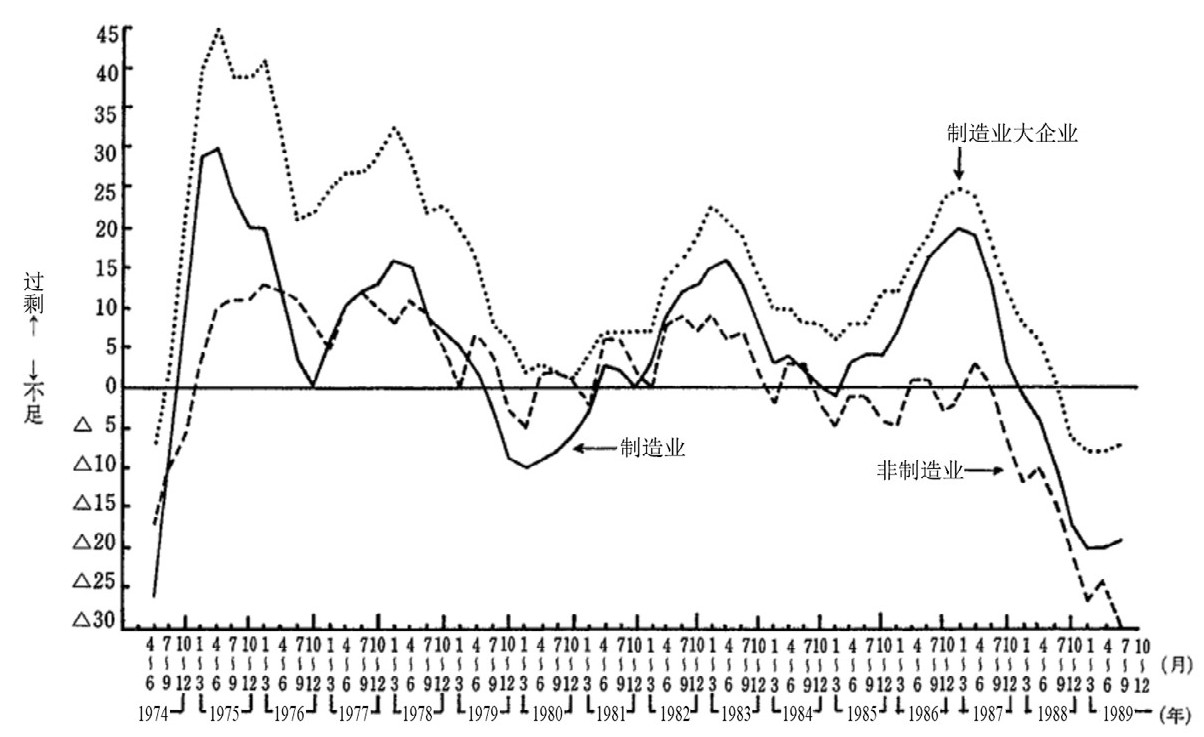
\includegraphics[width=\linewidth,keepaspectratio]{image/2-1日本全行业劳动力紧缺指数.jpg}

\caption[日本全行业劳动力紧缺指数]{日本全行业劳动力紧缺指数\protect\footnotemark}\label{fig:2-1}

\end{figure}

\footnotetext{参见厚生劳动省白皮书《平成二年版労働経済の分析》。}

在人才最为紧缺的1989年，厚生省的统计数据显示：全行业岗位缺口高达500万个，其中房地产行业一枝独秀，岗位缺口接近300万。而当时全国适龄劳动人口才刚刚超过6000万人，这意味着需要凭空多出10\%的人口才能填补岗位空缺。在这样的背景下，就业市场的竞争异常激烈，不仅名校大学生备受青睐，就连最普通的私立大学毕业生也能轻松找到理想的工作。

当时日本最大的房地产公司，西武集团的总裁堤义明在这种人才紧缺的环境下，提出了所谓“奴才哲学”，他认为只要招聘足够多的员工来执行他的命令，就能拓展商业版图。令人唏嘘的是，这个曾经拥有15万名员工的集团，泡沫破裂后成为全日本失业员工数量最多的公司之一。2005年，由于长期的财务造假，堤义明最终锒铛入狱，盛极一时的西武集团也逐渐消失在了历史的长河中。

1989年就业白皮书明确指出：大学生已经出现严重供应不足，供需矛盾至少需要5年的时间才能缓解。然而这篇报告的作者肯定无法料想，2个月后日本将迎来股市的“大纳会顶点”\footnote{“大纳会”，即股市每年的最后一个交易日。在日语中，“纳”意为“结束、收尾”，“会”指“交易时段”。}，泡沫经济达到最终章。而报告中描述的让人兴奋的大学生就业前景，在3年后成了全行业雇佣过剩。1992年就业白皮书披露，相比较1989年，员工的平均利用率和劳动密度都出现大幅下降。

然而，由于日本企业普遍实行的终身雇佣制度，企业很难对老员工进行裁员。因此，为了应对劳动力成本的压力，企业纷纷选择暂缓新员工的招聘。全社会开始出现大规模的缩招潮。

\subsection{二、房贷重压下的老员工与刚刚毕业的大学生们}

1992年日本企业的缩招潮开始蔓延，年底每个求职者对应新增岗位数量仅有0.73个，也就是所有新增岗位都招聘完毕，全社会依然可能有27\%的人处于待业状态。而在2年前这一数字却是1.5，仅仅两年时间全社会岗位数量就缩减了五成。由于此时日本企业采用年功序列制（终身雇佣制），老员工为了工龄累积几乎不会离职，当时的求职市场主要由每年的大学毕业生构成。

因此，大学生成了这次岗位缩减潮最大的受害者，而谁也没想到的是这一轮缩减潮居然持续超过10年。2012年随着《失落的二十年》一书爆火，这一批从1993年至2003年毕业的大学生后来有了一个统一的名字，那就是失落的一代人，意指被日本社会牺牲的一代人。

那么为何不能牺牲老员工的利益，打破这些老人的终身雇佣制？

除了制度的本身限制以外，真正的原因是如果马上启动对现有就业群体的改革，很有可能会引发金融风险。经过全民炒房热潮后，日本家庭平均负债是年收入的3.1倍，即每个家庭都透支了未来3年的收入。而地产暴跌后，银行业坏账率已经逼近5\%的临界点。如果日本政府现在启动改革，必然产生大量的失业断供，此时的金融体系已经无法承担这样的坏账率冲击，这也是日本政府一开始并不愿意打破终身雇佣制的原因。

那么当时日本这群老员工的债务问题有多恐怖？

1985年广场协议签订当年，日本银行贷款总额为267万亿，而到泡沫巅峰的1989年已经暴涨到410万亿，超过当年国民GDP。其中有大量贷款都是30年以上的个人超长期房屋信贷。

这就带来了一个可怕的问题，泡沫最疯狂阶段整个银行体系在4年时间增长了140万亿贷款，但在泡沫破裂之时这些贷款还款周期大多都不到20\%。这就意味着一旦老员工们失业，他们这剩余80\%的未偿贷款将只能由银行消化。从后来的发展上看，90年代后期日本银行确实遭遇了不良资产危机，但那场危机主要来自企业端债务暴雷，就这已经让银行业元气大伤，全行业在2010年后才逐渐走出衰退影响。试想一下，如果企业端与居民端同时暴雷，日本银行体系大概率将尸骨无存。

也正是由于日本政府维系住了现有就业群体的稳定，再加上工作与信用的强绑定关系（日本正式员工评判最重要的就是个人信用健康），即使老员工们的资产早已大幅贬值，他们也愿意用余生还完这些超长期贷款。后来这群人还有一个很自嘲的说法，因为日本房屋抵押贷款合同一般称为“住宅契约书”，所以他们是用一生还完了自己在30岁时签下的“魔鬼契约”。而这也是日本政府一定要优先保证老员工就业的原因，因为这让日本避免了居民端的债务暴雷。

但笔者必须强调，尽管日本政府对老员工们多有优待，但也并不是一开始就打算完全牺牲大学生群体的利益，政府初期更多的是采用延缓就业的形式来拖延大学生就业。如果站在决策层角度思考，假设后面的经济能够重新恢复增长，那么延缓大学生就业的选择是正确的，这样可以同时保住新老就业群体。

只是日本政府怎么也想不到，这一轮经济衰退居然持续了20年这么久。

\subsection{三、延缓就业之痛}

1992年至1995年间，面对大学生就业的严峻形势，日本政府推出了“乡村分流”与“研究生扩招”两项举措，旨在尽量延缓大学生进入就业市场的时间，以缓解就业压力。

乡村分流方面，日本政府启动了一项为期3年的乡村基建计划，积极鼓励大学生前往非都市圈区工作，这一举措后来被称为“逃离东京运动”。厚生省统计通过分流政策，3年间成功将近30万大学生分流到乡村和小城市，既大大减少了东京的就业压力，同时也为乡村地区带来了新增人口。而在扩招政策上，日本政府迅速放宽了大学与研究生门槛。1992年日本在校大学生还只有237万，而3年后就增加到了310万，3年时间整个大学体系增加了73万学生。同时日本大学生深造比例开始升高，研究生门槛的降低使得1995年64\%国立大学生都选择读研。

根据日本文部省统计，1992年至1995年间，通过乡村分流与扩招两个措施，至少延缓了约90万大学生进入就业市场。这也为日本政府保就业争取了宝贵的时间。1995年开始，日本新增岗位数量触底反弹，大学生们的就业似乎迎来了希望的曙光。

然而看似美好的希望，却隐藏着一个巨大的隐患。毕竟政策只是拖延了大学生的就业时间，但最终，这批大学生还是要面对就业的现实。

从1996年开始，日本政府逐渐停止了大基建投资，原先创造的大量乡村岗位迅速消亡，大学生被迫重新回到大城市就业。据统计在1996年至2000年的五年间，仅东京就新增了27万人口，其中70\%是毕业5年内的大学生。而更可怕的是1996年日本迎来了扩张后的第一轮毕业潮，全学历段待业总数达到惊人的80万，同时还有260万在校大学生等待毕业。此时日本经济还在衰退，就业市场根本无法承受如此巨量的大学生规模，当年大学生就业率瞬间下降至65\%。

1996年，日本社会已经深刻意识到危机的来临。面对数百万待就业的大学生，日本政府清楚地认识到，大学生就业潮已经无法再被拖延。

就业市场必须进行改革了，但这次改革的第一刀却又砍向这批大学生群体。

\subsection{四、劳务派遣之痛}

1996年政府修改了《工人派遣法》并推广劳务派遣制度，鼓励企业减少正式员工雇佣比例，将临时员工作为新的就业蓄水池。这轮改革后，所谓的终身雇佣制度基本就与大学生无缘了，此后10年日本每两个大学毕业生就有一个是临时员工。

但比成为临时工更可怕的是，这轮改革也基本摧毁了日本企业的用人价值观。

既然企业可以随意裁减临时员工，大学生被要求一毕业就要具备即战力，企业对于新人犯错的容忍度几乎为零。甚至可以说大学生一毕业，就面临的是一个毫无晋升空间的职场环境。据统计，这批临时员工在10年内成功转正的比例仅有47\%。这种环境下，新人们怎么可能规划好自己的职业生涯，多数人被迫开始频繁跳槽。而此时日本社会还没有意识到这批大学生其实才是真正的受害者，反而认为这批大学生不够努力、不够上进，由此催生了“垮掉的70后”。可以说，这一代大学生没有赶上终身雇佣制度的红利，但却成了终身雇佣制度解体的牺牲品。

日本政府之所以会这么改革，一方面是因为老员工的终身雇佣已经是既定事实，既得利益群体难以撼动。更重要的是，此时银行的不良率已经超过5\%的危险线。如果启动大规模裁员，企业需要支付大量赔偿金，而失业员工则可能引发房贷断供。这样一来，企业端与居民端的负债将同时暴雷。

因此在债务暴雷与大学生的抉择之间，日本政府再一次选择了牺牲大学生群体的利益。毕竟，这批大学生的父母都是团块世代的有钱人，他们可以为子女支付生活费，因此这批大学生在物质上并没有出现太多危机。在我国，他们有一个新的称呼，叫作“全职儿女”。

然而，相比较职业上的不顺利，这批70后大学生的内心却出现了更严重的问题。

此时已经是泡沫破裂后的第5年，很多大学生已经意识到，即使再努力，原本规划好的人生也无法实现，宅文化开始兴起。而反映这种心态最明显的例子，就是电视剧《悠长假期》的爆火。1996年，这部讲述两个东京失业年轻人的电视剧创下了30\%的惊人收视率。剧中木村拓哉那句“在自己什么都做不好的时候，就当是上天赐予的一个长假”的台词，安抚了很多年轻人的内心。要知道，在5年前，日本最火爆的电视剧还是《东京爱情故事》，那是一部讲述乡下孩子在东京打拼、催人奋进的励志电视剧。仅仅相隔5年，两部电视剧的对比就能说明当时日本年轻人心态转变之快。

也许看到这里，你会觉得日本的大学生们已经过得很惨了。但你要知道，1992年至1996年，日本还处于泡沫经济的惯性中，家庭中位数收入还维持在550万日元的历史高位。虽然工作辛苦了一点，但起码家庭收入是没有下降的。简单来说，没有工作的孩子至少还有父母可以依靠。

但苦难就仅此而已吗？

\subsection{五、金融危机之痛}

当1997年新年的钟声敲响，日经指数重新站上21000点大关。这一短暂的复苏的状态，让整个日本社会都误以为经济已经重新步入增长的正轨。政府发布的白皮书甚至开始预警，称存在经济过热的风险。大学生们也纷纷开始憧憬，自己的人生终于要重新回到正轨了。

然而，正当所有人都沉浸在希望之中时，亚洲金融危机的突然爆发，却如同一场无情的风暴，瞬间打碎了所有人的美梦。以日本四大券商之一的山一证券倒闭为起点，日本政府拖延了近7年的银行坏账问题终于迎来了爆发。坏账率迅速逼近10\%，日本金融体系开始崩溃。

金融大爆炸时期日本总计倒闭153家银行，未倒闭银行的累积亏损达到11万亿日元。由于银行业在日本百业之母的地位，大量实体企业与银行其实是共生状态，因此每倒闭一家银行就会连带许多企业濒临破产。由此1998年3月日本创下了单月破产1820家企业的历史记录。

在此背景下别说大学生的稳定就业了，海量社会精英都因企业倒闭失去工作。

当年，仅山一证券的破产案，就导致了1.2万名员工失业。而山一证券最后一任社长野泽正平，那张他哭泣着恳求大家帮助失业员工再就业的照片，后来也被视为日本泡沫经济正式破灭的象征。

如果说1997年之前，日本社会还处于有能力但不主动解决大学生就业问题的状态，那从1997年的金融大爆炸开始，日本政府的决策层就真的陷入了自顾不暇的境地。由于处置危机不力，5年间日本政府更换了4位首相，最终只能通过超发40万亿日元的债务来救助企业，这才勉强控制住了这次危机。

然而，在这样的混乱局面下，谁还记得那些大学生们怎么样了呢？

在1997年至2003年的这段时间里，日本社会从上到下，已经没有人再去关注大学生的处境了。毕竟，需要拯救的倒闭企业实在太多，大学生的就业问题，自然就被排在了优先级的后面。最明显的一个例子就是，在这5年时间里，日本政府甚至没有出台过一部专门针对大学生就业问题的法案。

而这也是这批大学生后来被称为被遗忘一代的原因。他们就像被忙着救火的大人们遗忘在角落的孩子一样，被整个日本社会所遗忘。2003年日本大学生的就业率已经跌到令人发指的55\%，即每年的毕业生中，将近一半处于失业状态。

那么经济好转之后，他们的人生能变好吗？

\subsection{六、被时代遗忘的一群人}

2003年后日本金融大爆炸的影响开始消退，日本政府重新鼓励企业雇佣大学生，全职雇佣人数与岗位比例均显著上涨，2007年大学生就业率重新回到70\%。但此时一个尴尬的现实是，就业冰河时期的学生们基本都已经毕业超过10年，即使校招恢复，又与已经做了10年临时工的他们有何关系！

而在社招市场上，此时就算老员工们已经退休了，优质的岗位依然与这些90年代的大学生无关。

2004年，随着团块世代进入退休阶段，日本再次掀起了“再雇佣”的风潮，一批老技术员工被返聘成为香饽饽。这是因为企业发现，这些老员工经历过七八十年代众多项目的历练，往往拥有更丰富的工作经验和专业技能。相比之下，90年代的大学生在毕业后面临的是产业与技术的衰退，他们中的许多人不要说历练了，甚至都没有完整参与过几个项目，自然也谈不上什么专业的技能。更糟糕的是，不少公司宁愿选择刚刚毕业的大学生重新培养，也不愿意培养一个老人。而这批70后因为年龄过大，就算是正式员工，也已经沦落为下一批“窗边族”的储备。

根据厚生劳动省统计，“失落一代”在35岁的收入比泡沫经济时期的毕业生低25\%，也低于就业冰河时期后的毕业生，成为三代人中的收入最低的群体。

后来，知名作家小林美希这样总结这一代人：他们出生于20世纪70年代的日本婴儿潮时期，学生时代见证了日本80年代的经济腾飞，但却在毕业后迎面撞上90年代无止境的经济衰退。最终，他们成为日本收入最低、结婚率也最低的群体。

至此，第二章的内容就结束了。前两章我们回顾了在失业潮的大背景下，日本政府在企业发展与社会稳定之间的抉择，以及面对新老世代不同困境所做出的取舍。这两章的讨论主要聚焦于城市，那么同样在失业潮的背景下，日本的乡村又发生了怎样的变化？
 \cleardoublepage
    % 来源：EPUB spine / EPUB/xhtml/chapter2_0003.xhtml

\BookChapter{3}

\section[第三章\q 留在城市还是返乡的选择]{第三章\\ 留在城市还是返乡的选择}

\BookSubtitle{——回顾日本返乡就业潮：日本漂流一族的故事}

{\fangsong 由于无法在大城市获得一份稳定的工作，却又难以回到自己长大的故乡，他们被迫放弃婚姻、生育与房产，持续不断地失去，成为那批人最真实的写照。\par}

{\fangsong 回不去的故乡，留不下的都市，夹在城市与家乡间的漂流一族究竟是如何诞生的？\par}

2019年《平成的教训——改革愚策》在日本书市悄然上架，作者竹中平藏作为小泉纯一郎内阁时代的“经济沙皇”，在2001—2006年间以雷霆之势亲手解决了“金融再生”与“邮政民营化”两大不可能改革，被赞誉为小泉改革的总设计师。得益于财政改革的成效，竹中平藏在任内短暂实现的“小泉经济景气”，也被认为是90年代泡沫破裂后的首个真正意义上的景气周期。

但当这位铁腕改革家再次总结平成时期历次改革的得与失时，却将一大部分篇幅放在了另一场改革上。那就是如今依然在日本社会争议不休的“乡村振兴”以及后续引发的“平成大合并”。

最近几年在中国，年轻人要不要回老家工作的话题越来越火热，很多人开始讨论是否应逃离一线城市，回到家乡就业，而这也恰恰是日本90年代那批年轻人面对的选项。当年那场返乡就业潮，给我们留下了哪些经验与教训？

\subsection{一、经济崩溃后的城市就业困局}

1992年日本经济增长率下跌至0.9\%，高速发展的城市经济被瞬间按下停止键。增长的戛然而止，让泡沫经济时期吸纳海量年轻人就业的东京、大阪、名古屋三大都市圈，即刻迎来了严重的劳动力过剩。至1993年，三大都市圈的求职总人数是岗位数量的1.46倍，即所有岗位都招聘完成也只能消化70\%的求职者。

一个严峻的问题摆在全社会面前：经济快速增长的时期，大城市尚能吸纳大量涌入的年轻就业者；但当经济增长不再持续，这些青年却依然滞留在大都市圈。数据显示，泡沫经济时期仅东京一地每年就涌入超过12万青年，而随着经济下行，各大城市的青年失业率开始快速上升。

在此背景下，日本政府启动了一系列举措用以分流城市人口，鼓励年轻人返乡就业，后来这些举措被统称为“日本乡村振兴计划”。根据农林省统计，整个乡村振兴计划期间总计有四百万人回到乡村就业，东京连续三年人口负增长，短时间内缓解了城市就业压力。但从后来的数据来看，乡村振兴运动仅维持了7年就匆匆宣告结束。

计划结束后，海量年轻人回流都市，此时恰逢第一章与第二章提到的日本金融大爆炸后的企业破产潮。海量返城人口与城市失业潮的叠加，直接引爆了日本2000年的超级就业危机。2000年至2003年，也被日本社会称为超级就业冰河时期，意指泡沫破裂以后日本就业最困难时期。

那么为何看似美好的年轻人返乡就业潮，最终却诱发了日本的就业危机？其实日本启动这一轮乡村振兴计划，还有一个原因是希望通过大基建来刺激经济。过去20年日本核心都市圈已经基本完成建设，这一轮刺激只能将乡村作为基建的蓄水池。因为这既能快速创造就业岗位降低失业率，还能够分流城市人口。

此外，当时进行乡村振兴计划还有一个原因，那就是平衡泡沫经济时期畸形的大城市过热现象与地区分配的严重失衡。当时三大都市圈对资本形成了巨大的虹吸效应，1986年至1990年，三大都市圈的资本增资达到1000万亿，而其他中小城市合起来也才200万亿。

但从居民分布上看，三大都市圈即使算上所辐射的卫星城市，其居民占比也才略微超过40\%。与其说整个泡沫经济是日本的狂欢，倒不如说是大都市的狂欢，甚至可以说仅是东京一个城市的狂欢。站在当时决策层的角度考虑，乡村振兴计划既能创造大量乡村就业，又能刺激经济增长，还能将都市圈聚集的资本驱散到地方，从而实现不同地区的再平衡，可谓一石多鸟。

但谁承想后来经济迟迟没有恢复，海量人口的持续返乡迫使政府只能不断维持基建规模，最终乡村无法承受过剩的人口，地方的财政也不堪重负，导致了后来著名的平成大合并。大合并后日本乡村一半的基层岗位消失，无数年轻人被迫回到大城市沦落为漂流一族，这个后文将会提到。

我们先说说日本是如何刺激年轻人返乡就业的。

\subsection{二、第一轮返乡潮：乡村大基建计划}

1992年日本政府推出著名的乡村基建振兴法案，而经历了20年房地产高速发展的我们，都已经知道基建对于就业的带动效应。根据大藏省统计，1992年至1995年有25万亿日元流向乡村基建市场，建筑从业者成了这一计划最大的受益者。

从相关数据来看，在1990年六大都市房地产遭遇断崖式崩盘的严峻形势下，建筑业从业者数量却逆势上扬，从泡沫形成前的510万人稳步增长至1997年的700万人，堪称日本泡沫破裂前7年间从业人数增长最为迅猛的行业。直至1995年第一轮乡村基建投资圆满完成，据日本总务省统计，在1992年至1995年期间，每年有70万人从都市圈向非都市圈迁移，而建筑行业从业者在这一迁移群体中占比超过一半。

在大规模基建项目的有力刺激下，到了1995年，日本的GDP增长率终于回升至2\%以上。然而，即便如此，当时核心都市的失业率依然居高不下，超过了3.5\%，城市的就业压力依旧巨大。

因此决策层只能选择继续进行大基建计划以分流城市过剩的年轻人。

其实日本政府十分清楚乡村大基建的危害，其1995年的经济白皮书已经明确指出：过量的基建投资并没有被有效用于民生建设，其对于国民经济增长的刺激效果已经十分微弱。并且每个地区为了尽可能争取到基建预算，大量的无效建造项目被提出与实施，乡村大基建计划演变成了各个地区利益党团的肥肉，最终导致至今都在影响日本社会的“乡村公建”党团的形成。

后来日本社会形容：这是用混凝土将乡村重新包裹了一遍。最明显的例子就是，全日本55\%的海岸线都被混凝土覆盖。但日本当时陷入了两难抉择，如果马上停止基建，则通过基建创造的海量乡村岗位就会迅速消失，此时核心都市圈不可能承受如此多的人口转移。而如果继续采用大基建刺激则还能够延缓一段时间，以等待经济的好转。

1995年为进一步刺激经济，政府推出14万亿日元的一揽子再刺激计划，再加上1995年底阪神地震重建计划，日本进入了新一轮的投资热潮。而央行还在不断火上浇油，将银行贷款利率一口气下调至0.5\%，日本乡村大基建的狂欢进一步持续。

\subsection{三、第二轮返乡潮：乡村旅游振兴}

1995年在持续高压的城市失业率下，政府只能继续刺激乡村就业市场，只是这一轮从基础建设转为乡村旅游投资。当年推出乡村休闲促进法，鼓励民间资本在乡村建设度假村等休闲设施。

此后乡村旅游马上成为日本最大的投资风口，而日本银行恰好苦于无人贷款，因此海量的银行贷款也马上涌入乡村旅游行业。海量贷款进一步刺激了乡村旅游市场项目，根据日本旅游局数据，法案推出6个月后，全日本新增开工了109个大中型度假村。

而1998年的长野冬奥会又进一步刺激了乡村旅游的投资热情，当时全社会热炒滑雪运动与冬日度假村的概念，至1998年全国仅滑雪场就有700座，几乎每个乡村都在发展特色旅游项目。而长野地区更是成为乡村旅游胜地，人口仅37.8万的长野市总计吸引了105亿美元投资，折合日元超过1万亿，成为当时乡村振兴的典范。国际奥委会前主席萨马兰奇甚至评价：长野冬奥会不仅是一次体育上的巨大成功，还是一个小城市的经济发展机遇。

但笔者需要强调，乡村振兴与乡村旅游本质上还是在房地产信贷持续萎靡的情况下，为了刺激经济投资，民间资本与政府资本共同参与的结果。但只要有债务，就必然要偿还。不过这个话题我们稍后再说，先说说这轮乡村旅游投资取得的成就。

这一轮乡村旅游潮，同样带动了海量人口返乡就业，但与之前大基建带动建筑业人回流不同，这一轮乡村旅游热潮带动的是大量服务业人口返乡。1996年各项新建旅游项目开始进入实际运营阶段，乡村中高附加值的旅游业收入开始增加，日本城乡之间的贫富差距开始迅速被缩小。

至1997年，得益于旅游业的收益，日本农村家庭可支配收入达到历史最高值，恰逢城市处于1997年亚洲金融危机后的裁员降薪潮，日本农村家庭收入达到了城市工人家庭的1.26倍，这更进一步刺激了民众的返乡就业意愿。在整个就业冰河时期，为什么会有大量的年轻人返乡就业？因为一边是都市圈高昂的生活成本与失业率让他们无法喘息，而另一边则是回到自己的故乡还能够享受因为基建带来的高收入，很多人都会选择放弃城市的生活重新回到家乡。试想一个在一线城市没房没车的年轻人，在老家拿到一个比现在工资高的工作，任谁都会十分心动，毫不犹豫地回去。

但我们不要忘记了：“命运给你的礼物，其实早就在暗中标好了价格。”要知道整个日本的返乡就业潮都是建立在巨量的基建投资与海量民间资本之上的，其中很多岗位都是通过人为创造出来的，一旦投资停止这些岗位就会迅速消亡。1998年随着亚洲金融危机的进一步冲击，日本迎来了泡沫破裂以后最大的破产潮，日本政府被迫超发海量债务用以拯救城市中倒闭的企业。

而对于乡村来说则带来了两个巨大的冲击：第一是海量基建资本从乡村抽离用以挽救倒闭企业，第二则是大量通过银行贷款修建的度假村由于银行体系的破产同样迎来了倒闭潮。简单来说乡村这套长期依赖举债基建的模式无法运行，由此用大基建营造出来的乡村就业繁荣开始破裂。

至1999年日本终于出现了严重的地方债务危机，当年各地债务总额达到了恐怖的180万亿日元，是1989年的3倍，仅仅10年，日本各地就新增了120万亿债务。在巨大的债务压力下，别说是继续承担各类基础设施的运营费用，很多日本乡村甚至丧失了基本的偿债能力，只能依靠中央的财政支援维持运转。

还是以长野为例，这个因为冬奥会盛极一时的城市，在冬奥会结束后的第二年，就因为庞大的债务问题迎来了巨大的经济滑坡。1999年长野的制造业以30\%的速度下降，211家企业宣布破产，下降速度创造了二战以来地方经济衰退的最高纪录。冬奥会后，海量投资的餐馆与酒店更是空无一人，此后长期的债务问题让长野一度成为因举办奥运会濒临破产的城市之一，后来更是有了“长野的诅咒”一词。但有严重债务问题的，又何止长野一个地区。

根据内阁官房下设人事院统计，1999年有20\%的乡村，中央援助占到每年财政收入的50\%以上，很多乡村已经无法创造收入，但中央政府依然要支付高昂的运营费用。要知道中央财政此时也已经十分困难，海量的城市企业也需要中央财政援助。在财政极度困难的情况下，减少财政支出与缩减各地岗位成为必然的选择。

于是从2000年开始日本政府终于下定决心，启动了那场后来被无数人所诟病，也被无数人认为是拯救了日本乡村的“平成大合并”。

\subsection{四、返乡潮终局：平成大合并}

如今平成大合并在日本依然是一个很有争议的话题，我们这里不进行评价。平成大合并虽然拯救了日本乡村财政，但未能惠及依赖财政支出的群体，尤其是90年代就业返乡潮中的年轻人。2000年以后，日本在短短7年时间将原有的3200个乡村合并缩减至1700个，同时47\%的地方基层机构也在此轮合并潮中消失。根据日本官房厅统计，大合并完成后，全国仅人事支出一项每年就减少了1.8万亿日元，由此可见此轮合并潮中减少的基层岗位数量。

事实上平成大合并在日本还有另一个名字：“平成雪崩”。在合并潮中，很多人就像遇到雪崩一样，根本无法躲避就被裹挟其中。

随着平成大合并的开始，日本90年代的就业返乡潮被正式画上句号，海量乡村就业者重新回到都市。2001年东京的人口净流入量时隔12年重新突破12万人，并持续攀升至2007年的16万人。要知道2000年日本城市刚经历金融机构破产潮的洗礼，如此巨量的人口返城直接推升全国失业率突破5\%大关，各大都市圈聚集了大量待业人群。这段时间也因此被日本社会称为“超级就业冰河时期”。

此时的日本城市就业市场，别说高薪的工作了，就是正式稳定的工作也是寥寥无几。在超级就业冰河时期，日本的劳务派遣市场规模每年上涨30\%，而这批回到城市工作的年轻人们大多都是从事这类低薪且不稳定的派遣工作。据《日本经济新闻》2002年的报道，平成大合并后的返城者，部分甚至在从事便利店员工这样的低薪工作，要知道他们很多人曾经都是名牌大学生，可如今回到城市却只能从事这样低薪且没有前途的工作。

后来这些出生在非一线城市，生活在东京却只能靠打零工生存的年轻人，被日本社会称为漂流一族。2006年随着NHK纪录片《穷忙族》的播出，以这群人为原型创作的《工作漂流》与《中年漂流》，成为日本的系列畅销书。由于无法在大城市获得一份稳定的工作，又难以回到自己长大的故乡，他们被迫放弃婚姻、生育与房产，持续不断的失去，成为那批人最真实的写照。

可以说从时代的角度来看，他们是小镇青年通往大城市的最后一代人。在他们之前的一代人已经完成了在大都市的原始积累，而在他们后一代的人已经充分意识到大城市生存艰难，从而主动选择了平淡的人生剧本。

2021年随着《花束般的爱情》这部电影在日本爆火，这部由《东京爱情故事》编剧坂元裕二时隔30年撰写的故事再次引起了全日本的社会大讨论。这两部剧讲述的都是乡下孩子与东京女孩的恋爱故事。只是30年前我们看到的是在东京的拼搏奋斗，而30年后看到的则是年轻人在大城市不断碰壁后最终选择离开的故事。

这相隔的30年，也恰恰造成了三代年轻人心态的转变。

\subsection{拓展阅读}

\subsubsection{日本出租车司机如何走向饱和}

{\fangsong 21世纪后，随着返乡潮的人数加剧，日本失业率突破历史最高的5\%，尤其是城市淤积了大量失业人口。为此，政府在2002年修订了运输管理法，大幅降低了出租车行业准入门槛，促使海量失业人口涌向此行业。据厚生劳动省统计，行业就业峰值时，全国出租车总就业人数达到34万人，成为日本城市就业的一大蓄水池。\par}

{\fangsong 新的运输管理法实施后，出租车从业人数持续增长，至2009年达到历史最高峰，较2002年增长了22.3\%。出租车辆增长速度是此前就业冰河时期的1.8倍。由此可见在出租车门槛放开的第7年，出租车蓄水池将达到极限。\par}

{\fangsong 但需要强调的是，之所以日本出租车行业规模在增长22\%以后就陷入停滞，最主要的原因是过量从业者的涌入，导致收入降至难以维持生计的程度。那么收入下降到哪个程度，出租车蓄水池就会达到极限？\par}

经济增长时期出租车司机收入水平（1989年前）

{\fangsong 以东京都市圈为例，1989年的泡沫经济时期，出租车司机与东京全口径平均收入比高达0.9，而全口径中还包括了东京大量科技金融业高薪职员。因此泡沫经济时期的出租车司机是标准的城市中产，其收入能够达到社会的平均收入水平。\par}

就业停滞时期出租车司机收入水平（1990—2002年）

{\fangsong 但从1990年泡沫破裂后，由于消费降级，民众用车需求减少，出租车司机收入也相应减少，至1999年出租车司机与东京全口径平均收入比降为0.73。虽有降幅，但相比较失业，此时从事出租车司机仍然是一个收入稳定的选择。其收入水平依然高于货运司机。\par}

从业限制放宽时期出租车司机收入水平（2002年以后）

{\fangsong 从2002年放宽出租车从业门槛以后，随着海量出租车司机涌入，出租司机收入迅速降低。最低点出现在2009年，出租车司机与东京全口径平均收入比暴跌至0.54，即收入仅有城市普通居民平均收入的一半。\par}
 \cleardoublepage
    % 来源：EPUB spine / EPUB/xhtml/chapter3.xhtml

\BookPart{第二篇}{无法与自己和解的一代人}

\BookPartImage{image/第二篇无法与自己和解的一代人.jpg}
 \cleardoublepage
    % 来源：EPUB spine / EPUB/xhtml/chapter3_0001.xhtml

\BookChapter{4}

\section[第四章\q 人生开启于失落经济]{第四章\\ 人生开启于失落经济}

\BookSubtitle{——就业冰河世代的一生}

{\fangsong 团块次代，指的是日本20世纪70年代第二次婴儿潮期间出生的大约1800万人，他们自出生便被烙上“过剩”的烙印，从小学一路竞争到大学。但不幸的是，当他们步入社会时恰逢泡沫经济崩溃，一次次改革让这代人始终被时代浪潮裹挟，既未能继承父辈的经济红利，又无法获得后代的社会保障，成为日本“失去的三十年”的夹心层。\par}

{\fangsong 这就是日本的“团块次代”困境，这些人的一生都经历了什么？\par}

在日本劳动部的官网首页上，有一个醒目的标识，蓝色大字上写着“就业冰河世代特别支持”。\footnote{就业冰河世代特别支持：指为那些在1990—2000年泡沫经济破灭后，在困难的就业环境中寻找工作，面临各种挑战（就业冰河世代）的人提供支持。}当你点开进入页面，会惊叹其精美得不像一个古板的政府网站，鼓励话语与励志视频充满了整个角落，让每个第一次来到这个页面的人都有一丝莫名的感动。据日本厚生劳动省公布的数据，自2014年网站上线，其访问频率长期高于其他政府网站。很难想象这个温暖的网站的背后，却藏着一个日本社会过去30年不忍心谈论的群体。

自泡沫经济崩坏以来，日本就业形势严重恶化，在此期间走向社会的一代人被称为“就业冰河世代”。2024年，他们的平均年龄已经超过50岁，其中许多人终其30年都没有将自己的人生重新回拨到正轨，在贫穷与独身中，孤独地走过了半生。他们这段特殊的人生历程究竟承载着怎样的故事？又能为当下的我们提供怎样的启示？

\subsection{一、同辈压力竞争的70世代}

第二次世界大战结束后的头10年（1945—1955年），日本出现了一次巨大的生育浪潮，年出生人口一度攀升至260万，是2024年（72万人）的3.6倍，后来这一代人被称为“团块世代”。而团块世代的结婚和生育高峰恰好落在1970年至1980年之间。因此70年代日本进入第二次婴儿潮时期，10年间总计诞下了1800万新生儿，这一代人也被称为“团块次代”。

团块次代在出生之时被称为日本最幸福的一代，这是因为1960年池田内阁颁布了国民收入倍增计划，要求10年内国民生产总值及人均国民收入增长1倍以上。此后日本人均国民收入从1960年的395美元，增加到1970年的1592美元，10年间国民收入整整翻了4倍。全社会自此告别了国富民穷的年代。

20世纪50年代至70年代，美国作家傅高义用了20年时间写出了著名的《日本新中产阶级》。他以东京近郊的M町为叙述对象，完整记录了日本工薪阶层家庭的生活变迁：50年代家里只有五斗橱与床具，吃一碗酱油面都需要谦让；到60年代，城市家庭基本实现电视机、洗衣机与冰箱全覆盖的生活改善；到70年代，日本社会更形成了“一亿总中流”的国民共识，整体迈入中产阶级。可以说五六十年代坐着就业列车\footnote{就业列车：从1954年开始日本开行由中学老师带队，带着年轻人前往大都市就业的专门列车制度，该制度直到1975年取消。}前往大都市讨生活的乡村青年，确实为他们的孩子争取了一个美好的未来。

可以说当第一批70后出生的时候，他们享受的是亚洲最好的生活环境，而他们的父母则享受着高速增长的国民收入与十分低廉的房价。1980年前东京近郊地区的房屋总价通常不超过一个家庭年收入的6倍。

在这种美好的生活下，日本生育率开始一路高涨，1971年日本总和生育率达到2.16，即每对夫妇都会生育2个以上的孩子。那么这个数字有多高？在泡沫极盛的1989年这个数字是1.57，在超级就业冰河时期的2003年这个数字是1.29。低廉房价、高涨的收入与繁荣的经济成为日本最好的“催生药”。

但这也带来了一个问题，那就是巨大的同辈竞争压力。1971—1974年是战后出生人口的超级波峰，连续4年新生儿超过200万人，当时社会将其称为“800万团块次代”。而日本通常以四年作为一个同辈期，这800万新生儿在将来就变成了800万同辈竞争者。就此，“800万同辈竞争者”的概念，压在了当时每一个家长的心中。整个70年代日本都处于“回声婴儿潮”时期，随着战后第一代婴儿潮（1947—1954年）时出生的人陆续进入育龄，日本社会迎来新一轮生育高峰，新生儿数量累计超过1800万。

而在当时社会各界对这些新增人口普遍持乐观态度，将其视为日本新的人口红利。虽然人口众多会导致就业竞争会更加激烈，但这不过是经济繁荣期的正常现象。

\subsection{二、补习中度过的少年时代}

“四当五落”是一个曾经响彻日本70年代家长圈的流行语。考生每天睡四小时，就能考上自己心仪的大学（当），每天睡五小时的话，就会名落孙山（落）。日本七八十年代的大学录取人数仅有40万人，但当时每年都有140万人完成高中学业，实际的大学录取率不到40\%。但此时的社会，经济腾飞，索尼与东芝等大手企业在全球攻城略地，电视新闻上播放着日本企业世界第一的神话。而在求职报刊上更流行的一句话则是“大手企业千万年薪”。

日本泡沫经济极盛时期，顶级金融企业野村证券给每位社员的交通补贴高达400万日元，而中层干部则超过1000万日元。连交通补贴都超过千万，那工资得是多夸张的一个数字！日本社会开始疯狂追捧在大手企业工作。而当时进入大手企业的面试门槛只有一个，必须是一名大学生。面对如此巨大的诱惑与不足4成的大学升学率，日本发挥了儒家文化的核心技能“内卷”。1970年开始，日本教育市场进入了前所未有的内卷化状态。其实当时的教育内卷，除了要争夺大企业工作外，还有一个重要的原因：日本青少年正面临史无前例的“升学淘汰压力”。

简单来说，日本此时的年轻人太多了！本就珍贵的教育资源变得愈加稀缺。

当时日本教育体制仍然实行初高中升学考试，孩子们从小学开始就面临升学考试。由此也衍生了一个名词—“落ちこぼれ”。字面意思是“掉队者”，实际指的是那些无法跟上学校课业的学生。

1970年开始，东京地区优质私立初中，每年的申请人数都在录取人数的20倍以上。

今天回头看，日本家长对于子女教育的焦虑程度远比我们想象的严重，60年代至80年代日本是标准的学历社会意识形态，也就是大学层次直接决定了以后工作的优劣。1973年日本排名第一的东京大学入学致辞上有学生说：“我们将是改变日本社会的一群人”。这句话一时间轰动了全日本。虽然听起来有些狂妄，但也真实反映了顶尖大学生对于未来的高度自信。而在帝国核心的大藏省职员中，有一半以上来自东京大学与京都大学两大名校，顶级名校几乎与社会精英呈等号关系，当时这批人也被称为“学历贵族”。

学历社会中，一旦在学业考试上落败，基本等同于一辈子都毁了。在这样焦虑的心态与恐惧孩子失学的背景下，家长对于优质教育资源的抢夺进入白热化状态，而教培行业的爆发式增长就是这种焦虑最好的体现。

1970年日本教培行业正式进入所谓超黄金发展时期，1976年全国补习机构突破一万家，而仅仅5年后再次翻倍冲破2万家，10年时间机构数量翻了4倍。而在当时的“补习圣地”首都东京，出现了所谓封闭式补习集训班。那些头上绑着“努力必胜”的小学生们，都是每天睡眠时间不足6个小时，连续补习超过1个月。

傅高义曾经这样描写日本考试季的紧张景象：从考前一个月开始直至考试结束，是所谓的“考试季”。在这一时期，孩子成了家庭的绝对核心与焦点，妈妈会将热气腾腾的饭菜小心翼翼地放在托盘上，悄无声息地送至孩子面前，生怕任何一点声响会打断孩子的学习思绪，甚至连削铅笔这般再简单不过的小事也被妈妈揽在身上。

而父亲即使工作再忙碌，到这个考试季，上司也会让他们早早回家，辅导孩子的功课。整个社会，从社区的小商店，再到忙碌的办公室，再到会议时的闲暇，话题都围绕各自孩子的学习进度，探讨着不同学校的考试动态，每个人的脸上都写满了对这场考试的重视与关切。

而在大学考试成绩公布后，人们往往容易听到两种消息，一种自然是榜上有名的喜悦，另一种则是孩子接受不了落榜而自杀的惨剧。由于70年代，日本大学考试不会将成绩寄到家里，而是会张贴到特定的地区，因此看完榜单往往就知道是否考上。于是，日本社会形成了一种潜规则，那就是只能由父母代替孩子去看榜，因为担心孩子经受不住打击，在看榜回家的路上选择自杀。

70年代开始，考试竞争从小学到高中一路蔓延，景象之惨烈，被日本媒体称为“受験地獄”（应试地狱）。在这样的恐怖竞争压力下，在家长、老师、社会的焦虑中，这批孩子们打着鸡血度过了自己的少年时代。

\subsection{三、不被理解的青年时代}

不能被社会理解的一代，也无法和自己和解的一代，是日本知名作家小林美希给予70后的评价。

90年代开始，70后终于在焦虑与竞争中走完了大学时光，正当他们满怀希望憧憬未来时，却发现社会留给他们的不是“大手企业年薪千万”，而只有“就业冰河时期”。

关于就业冰河时期我在第一章已经谈过很多了，今天更想和大家聊聊当时的社会是怎么看待他们的。

如今的日本年轻人已经擅长应对经济衰退了，毕竟他们可是整整经历了失落的30年。“做好储蓄”“不乱消费”和“低欲望生活”是日本现在年轻人应对经济下行的三件法宝。可30年前，日本的大学可不会教这些东西，那时候经济持续增长，谁会教育一个学生如何在经济下行期间工作与生活？于是，70后成了日本经济下行期的第一代试验品。

高失业率、啃老族、御宅族在90年代就是离经叛道的代名词，毕竟80年代的昭和\footnote{昭和：日本年号，使用时间为1926年12月25日至1989年1月7日。}男儿们毕业就能去大手企业工作，过几年就能买车买房。怎么到了平成时代，年轻人就成了啃老族和御宅族，找不到工作天天呆在家里。“这一定是他们的问题，而不是这个时代的问题，是他们不够努力！”于是“不努力的70后”成了90年代的社会热词，如今稀松平常的御宅一族，在当时的日本社会可是大逆不道。因为现在的日本家长知道，孩子找不到工作是因为大环境不好，此外经历了30年经济下行期的他们，早已对孩子没有那么高的期望了。

但当时那批长期沉浸在鸡娃氛围中的家长们可不这么觉得：这都是因为孩子不够努力，只要他努力上进就一定可以找到工作。父母们按照年少补习时的路径依赖，不断给孩子们打鸡血，教导他们“天行健，君子以自强不息”。

于是这群70后陷入了自我证明的恶性循环，一方面父母与社会告诉他们努力就能成功，而另一方面自己明明努力了这么久却一点正反馈都没有。明明有好的学历却找不到好工作，理想与现实的落差使得他们既难以获得社会的理解，也无法与自己达成和解。在泡沫经济破裂的头10年（1991—2001年），他们长期处于社会的质疑声中。1997年开始，日本青年自杀率开始飙升，至2003年翻了近3倍，此后青年自杀人数常年保持高位。

当时三十来岁的年轻人没有工作、付不起房租、流落街头是一件很常见的事。而出于自尊，他们既不愿意求助父母，也很少申请政府救济。他们选择把一切的失败归咎于自己，再也没有与自己和解过。

但却无人告诉他们：其实不是他们错了，而是社会病了。

\subsection{四、被孩子厌弃的中年世代}

“我的父母就是废物”，今天的中文互联网开始流行“生物父亲”“废物开局”等词语，其本质上是一种对原生家庭的不满，是孩子对自己原生家庭财产情况的不满所衍生出的亚文化。而在十几年前类似的文化曾经风靡日本青少年，而孩子们所恨的，正是就业冰河世代的父母们——也就是那批少年时活在补习高压中，青年时活在就业困难中的70后们。

“派遣家庭”在日本社会是一个带有侮辱性的词语，用来指代父母都是派遣员工，工作十分不稳定、没有稳定的收入储蓄来源的家庭。在厚生劳动省2010年的统计数据中，70后有46\%的家庭至少有一方是派遣员工，而夫妻双方都是派遣员工的家庭比例也超过25\%，即日本每四个70后家庭，就有一个完全依赖不稳定的派遣收入。

而这种情况还在随着时间的推移变得愈发严重。被称为“团块次代”的70后，到2019年年龄最小的也已40岁。多数企业觉得他们精力不足，拒绝续签派遣协议，迫使他们从“派遣家庭”进一步滑落至“临时工家庭”。令和三年（2021年）日本国民贫困率是15.6\%，按家庭计算，每6个家庭就有一个符合国民贫困标准。而在单亲家庭中，贫困率则是44.5\%，也就是父母一旦离婚，孩子甚至要担心吃不饱饭的问题。

根据总务省2022年家庭预算年度调查报告，日本四口之家的每月的伙食费用是8.8万日元，也就是一年105万日元，而一个派遣员工年收入通常不会超过300万日元。这也是日本家庭主妇们个个都是省钱能手的原因，如果不是因为收入不足，有谁愿意晚上8点去菜市场抢便宜菜？此外，Good Neighbors Japan组织在2020年的一项调查发现，超过一半派遣家庭的父母将用餐次数减少到每日两餐，大约40\%的孩子在假期连一日两餐都做不到。

而比贫穷更糟糕的是祖父母的离世，派遣家庭很大一块收入来自祖父母（50后）的退休金，祖父母一旦去世，派遣家庭的收入马上就面临断崖式下滑。在日本，派遣员工的平均年收入是263万日元，而日本相对贫困线则是年收入200万日元，可以说大部分的派遣员工都挣扎在贫困线上。在派遣家庭出生的孩子们，从小就过着贫穷而备受歧视的生活。根据《日本经济新闻》抽样调查，派遣家庭长大的孩子中有61\%更对父母与社会存在仇视，而普通正式社员家庭的孩子只有27\%。

更可怕的是，派遣家庭的第二代们还普遍承受低学历困境。据文部科学省统计，日本国立大学4年学费是255万日元，私立大学则是550万日元。而派遣家庭的平均储蓄普遍在300万日元以下，这意味着孩子如果想要上大学，往往需要掏空整个家庭十余年的储蓄。而一旦考不上国立大学，家庭根本不能负担私立大学的高学费。

2007年日本电视剧《父女七日变》上映，这是一部讲述47岁的父亲与16岁的女儿灵魂互换，互相了解对方的生存境地，最后互相理解的故事。而这部电视剧的创作背景，正是当时日本子女仇恨父母最严重的时期。

日本的女孩子在幼儿园的时候最常说的一句话就是那句“等我长大了就当爸爸的新娘”，但是到了中学或高中又几乎不约而同的疏远并开始和爸爸保持距离。

\subsection{五、迷茫的老年}

如今，这批就业冰河世代走过了少年、青年与中年，正不可避免地迈向老年。2016年日本NHK纪录片《老后破产》上映，揭露了令人震惊的社会现实：日本独居的老人数量已逼近600万，其中约半数年收入低于最低生活保障标准。养老问题一时震动日本社会。然而这部纪录片的背后还藏着一个更严峻的问题：当这批就业冰河世代步入老年时，社会将如何应对？要知道《老后破产》讲述的群体还只是日本团块世代的老人们。而2030年，就业冰河世代们也将踏入自己的老年时代，面临的问题不论规模与复杂程度都远超前者，而这一次社会准备好了吗？

2006年，日本政府在东京开设了第一个专门援助窗口（就业塾），旨在为年轻无业者提供职业培训和就业帮助。设立之初，东京就业中心的“就业冰河期对策”主要面向20多岁的年轻人。

但时过境迁，主要的援助对象渐渐转为30多岁，甚至已是40多岁的人群。2010年日本政府将援助年龄上限提高到39岁，2018年上调至44岁，预计2025年将进一步提升到50岁。

“早上好！今天也要好好努力干！”2025年2月，伴随着活力满满的晨礼口号，东京就业塾又开始一天的职业培训，这样的口号已经持续了近20年。

只是喊口号的待就业者们，相比较20年前多了许多岁月的痕迹。

本章我们完整回顾了“就业冰河世代”的特殊经历。他们是婴儿潮与大学生扩招潮之间的一代人，为何学历没有帮助他们摆脱就业困境，他们中青年时代到底经历了什么，我们将在接下来的两章中详细探讨。
 \cleardoublepage
    % 来源：EPUB spine / EPUB/xhtml/chapter3_0002.xhtml

\BookChapter{5}

\section[第五章\q 学历贬值的一代]{第五章\\ 学历贬值的一代}

\BookSubtitle{——日本学历贬值的20年：回顾日本学历贬值史}

{\fangsong 他们是日本精英教育的最后一代人，从小接受“学历等于一切”的观念。他们也是日本鸡娃教育最严重的一代人，父母告诉他们知识才能改变命运，因此他们选择将自己的人生押注在教育上。\par}

{\fangsong 然而当他们踏入社会后，却发现自己用尽前半生换来的文凭，在泡沫破裂以后飞速贬值。\par}

学历的价值一直和大学生供应的数量息息相关。1992年日本社会迎来了第一批70后大学毕业生，但与上一代60后毕业就迎来泡沫经济繁荣不同，这一批70后们毕业就迎来了泡沫经济的破裂。整个90年代日本处于有史以来大学毕业人数最高的时期—1968年至1977年是日本的生育高峰，这波婴儿潮在90年代转化为大学生就业潮。据统计，90年代日本大学毕业人数整整比80年代多出40\%，而过量的大学生供应恰好遇上了日本就业冰河时期。

就业市场由此出现了一个严重的问题，在经济停滞，岗位减少的背景下，全社会却必须面对大学生集中式就业的冲击。于是日本政府在90年代中后期启动了就业与教育改革缓解供需失衡情况，但改革却导致了大学文凭的持续贬值，最终摧毁了日本社会曾经学历至上的思想。

从1994年至2004年的10年间，大学生起薪增长不到10\%，增长率甚至仅有同时期高中毕业生的三分之一。这导致大学生与高中生的工资水平被迅速拉近，社会开始出现大量的低薪白领阶层。后来这种学历快速贬值的现象，被日本社会称为“学历崩溃”，最终与“中产崩溃”以及“金融崩溃”，统称为“平成三大崩溃”。

在学历大幅度贬值以后，社会开始不再相信学历的价值。2024年全日本甚至仅有45万人参加高考，创下近30年历史最低值，高中生愿意参加高考的比例已不足50\%，其就业市场更是呈现低学历化。

那么日本这条学历贬值之路，到底是如何走过的？

\subsection{一、校招市场的崩塌}

从1992年开始，泡沫时期疯狂招聘大学生的校园招聘市场开始熄火。大量学生无法在校招期间找到工作，此后引发的校园招聘市场的崩塌也被认为是日本学历贬值的开始。

1992年，文部省统计当年还只有7万应届毕业生未能在校招期间找到工作，但到了1995年这一数字就提升到了17万人，占当年毕业总数的四分之一。短短几年日本的校园招聘市场就名存实亡，当时没有在校招期间找到工作的学生，只能被迫放弃应届生身份，在社招市场寻找工作。但毫无工作经验的学生如何与成熟工作者竞争？其薪酬与晋升必然严重受限。1994年日本大学生起薪涨幅仅增长1\%，远低于泡沫经济时期每年5\%的涨幅，还伴随着总体薪酬的大幅度降低。日本大学生学历开始进入贬值时代。

那么校招市场为何会崩塌？这是因为泡沫经济时期实施的校园招聘制度，已经无法适应经济下行的就业环境。就业协议规定，泡沫经济时期，日本大学采用的是限时招聘制度，每年只有8月至10月，大学允许企业到校园开展招聘签约，而其他时间禁止招聘。同时企业需要与大学生和学校签署就业内定协议，所有的招聘活动需要在大学的监管之下完成。

当时这么做主要是为保护企业利益。泡沫经济时期日本每年的人才缺口高达500万人，而当时一年毕业的大学生也不过50万。人才如此有限就必须限定招聘时间，避免企业恶意抬高薪酬哄抢大学生。但泡沫破裂后，日本企业利润下滑导致用人需求快速萎缩，1993年参与校招企业的数量更是比泡沫时期减少70\%。在没有足够校招企业数量的情况下，这一制度反而严重限制了大学生找工作。

简单来说，过去只需参加校园招聘会就能找到工作。但现在校招岗位大幅度萎缩，学生们一旦不能在规定时间内找到工作，就面临毕业即失业的困境。由此海量失业大学生，在社招市场形成了一个巨大的就业堰塞湖。而90年代日本社招基本由中小企业构成。中小企业对员工的压榨程度，想必今天的我们都有感受。这段时期大学生毕业3年离职率超过30\%，频繁的跳槽又加剧了学历贬值。至1995年大学生起薪出现30年以来首次负增长，学历贬值问题成为当年日本热议的话题。

就此，日本社会迎来了第一轮学历贬值浪潮。

\subsection{二、无序就业时期}

1996年日本社会迎来史上最大的婴儿潮一代就业冲击。

1973年破纪录的210万出生人口，在1996年转化为了恐怖的80万应届毕业生。面对已经名存实亡的校招市场与就业潮叠加，日本政府开启了第一轮就业改革，但这又加速了日本的学历贬值。后来这段时间被社会称为无序就业时期。

这一轮改革有两个方向：第一就是我在此前多次提到的修订劳务派遣制度；第二则是全面废除校招制度。

其实1996年的劳务派遣制度改革只开放26个工种，影响还比较有限，废除校招制度才是造成学历再次贬值的主因。从改革措施来说，改革后大学不再限制学生签署劳动合同的时间，企业可以在任何时间进行招聘。政府充分放任大学生与企业的招聘活动，即只要大学生能找到工作就可以。而这一制度在刚推出的时候确实取得成效：当年大学生就业率出现泡沫破裂后首次回升。

但在就业率回升的背后，学历贬值却进一步加剧。

此后日本的大学毕业生陷入恐怖的就业内卷中。由于校招制度废除，不再有固定的校招时间，这导致学生们反而被迫提早寻找工作。有些甚至在大一就参加各大企业的实习计划，从大一到大四几乎每个学生都在为就业进行准备。当时《日本经济新闻》将其称为就业军备竞赛，全社会出现了疯狂的考证浪潮。在这样的环境下，很多人甚至抱着找到工作就好的心态，根本不考虑工资的多少。由于大学生就业过于内卷，甚至出现所谓“大学生即奴才”的说法。而从数据来看，1997年日本大学生起薪再次出现负增长。

事实上，当时的学历之所以贬值，还有一个全社会都讳莫如深的原因：那段时间正是日本代际传承最严重的时期。

当时恰逢团块世代的子女就业潮，团块世代群体作为日本大手企业员工中占比最高的群体，自然可以很轻松地为子女寻找工作。据《日本经济新闻》统计，1998年日本1000人以上规模企业总计招聘了14万人，其父母是团块世代的占比超过50\%。

大企业本就是工资最高的所在，在市场岗位本就稀缺的情况下，这些优质的岗位还被“二代”们所占据，学历失去了竞争价值。后来愤怒的社会将这帮人称为上级国民，而没有权利的他们是下级国民。2002年随着动漫《名侦探柯南：贝克街的亡灵》上演，这部讽刺上级国民的动漫马上在日本被奉为神作，要知道此前的日本影视几乎不敢碰触这一话题，而这部动漫能够上映，也说明当时日本社会对代际传承的怨气之深。

其实我们并不能将日本学历贬值原因都责怪于制度改革，毕竟整个90年代都处于日本有史以来大学生人数毕业最高的时期，1968年至1977年本就是日本的生育高峰，婴儿潮必然带来大学生就业潮。而过量的大学生供应恰好遇上了日本就业冰河时期，学历贬值几乎是必然现象。

至1999年日本大学生月平均工资为19万日元，5年仅仅增长了3000日元。同时期日本初中毕业生月工资都增长了2.3万日元，由此可见当时日本学历贬值的速度。

就此日本学历完成了第二轮贬值。

\subsection{三、劳务派遣市场化时期}

但笔者必须强调，整个90年代日本的学历贬值还相对较慢，大学生的薪酬还能保持基本的稳定，考公或者返乡工作对大学生依然是个机会。

而2000年以后，才是日本学历贬值最残酷的时代，那就是超级就业冰河时期的学历贬值问题。

2000年开始，日本进入超级就业冰河时期，这时候城市有三类失业人口。第一类是日本银行破产潮后的金融工作者，第二类是返乡就业潮后的回城人员，第三类则是日本过去10年过量供应的大学生们。关于前两类我在过往章节已经回顾过，这里就不再赘述了。当时这三类失业人群几乎挤爆了日本的城市就业市场，2001年三大都市圈总失业人口达到了280万人。

就此日本启动了第二轮就业改革，而这一轮就业改革直接指向了劳务派遣制度，而这成为日本学历贬值第三阶段的开始。

1999年政府彻底放开劳务派遣制度限制，所有工种都可以进行劳务派遣。而2000年政府颁布《派遣机构管理法》，将劳务中介机构合法化，要知道日本此前介绍工作收费是不合法的。

改革后，劳务派遣彻底成了脱缰的野马不再受到监管。

从2000年开始日本进入劳务派遣市场化时代。此时就业市场的海量失业人口，对于劳务机构来说就像是秃鹫看到了腐肉，他们可以尽情地压低劳动者的薪酬。2001年日本人力机构联合建立了臭名昭著的劳务等级制度。制度将人公开地划分为ABC等级，不同等级对应不同时薪。而为了尽可能压榨价值，到了后来想被评为A级劳工几乎是天方夜谭。而学历在这种压榨制度下的作用十分微弱，在当时高中生与大学生被划分到一个劳务等级是十分常见的现象。

至2003年，30岁以下年轻人的劳务派遣比例高达40\%。

年轻人几乎都活在劳务等级制度的阴影之下，而学历在这种等级制度下作用越来越小。厚生劳动省统计，劳务派遣市场化以后，劳务派遣员工的月工资只有正式员工的40\%，而在东京这样的大都市基本只够温饱。

2007年电视剧《派遣员的品格》拿下了当年收视冠军，这是日本第一部揭露残酷派遣制度的电视剧。剧中女主角大前春子所信奉的，必须让自己强大到极限，掌握所有技能才能不失业的信念，其实就是派遣制度对人性摧残的象征。要知道女主角是日本名牌大学的毕业生，又在大银行工作过，但是因为银行破产失业，就沦落为一名派遣员工。

可以说劳务派遣的市场化彻底完成了对日本学历贬值的致命一击。

但你以为日本学历贬值的故事就此结束了吗？要知道由于社会对于学历认同的惯性，当时大家考大学的热情依然很高。虽然大学生毕业的工资不高，但毕竟文凭还是身份与知识的象征。那么日本高中生是什么时候开始拒绝高考，转而选择毕业就参加工作的呢？

\subsection{四、教育市场化改革}

2005年日本启动了大学法人化改革，后来这一改革被日本社会称为大学地震。这次改革的宗旨只有一个，那就是在长期萧条的经济下，日本财政已经无法供养现有大学了，政府要求大学增加收入，尽快实现自负盈亏。改革后，日本所有大学都选择增加学费，此后面对不断上涨的学费，读大学成了一件奢侈的教育投资。

2010年日本国立大学学费已经暴涨到53万日元，私立大学更是涨到80万日元。在学费如此高昂的背景下，贷款上学成了必然的选择。大学市场化改革后，日本每2.7个大学生中，就有1人靠助学贷款完成学业，其平均贷款金额高达300万日元。

但日本严峻的就业形势，导致很多学生毕业后还不上贷款。

贷款机构统计，2010年日本未按时还款的大学生们高达33万人。而这些大学生甚至还没有进入社会就迎来了个人的信用破产。2000年开始日本自杀率逐年提升，至2010年突破历史性的3万人，高学历的劳务派遣员工成了其中的主要群体。就此社会开始出现大批量的高中生就业群体，日本开始沦为低学历社会。

厚生劳动省统计大学市场化改革后，成为一个国立大学毕业生的终生总花费大约为5000万日元，私立大学则为8000万日元。而一个派遣员工终其一生的工资也不过1.3亿日元。

回望这批高学历者，他们是日本精英教育的最后一代人，从小接受“学历等于一切”的观念。他们也是日本鸡娃教育最严重的一代人，父母告诉他们知识才能改变命运，因此他们选择将自己的人生押注在教育上。然而当他们踏入社会后，却发现自己用尽前半生换来的文凭，在泡沫破裂以后飞速贬值。

但这批大学生就是最惨的一代人吗？读研考博真的能够改变命运吗？答案将在下一章揭晓。

\subsection{拓展阅读}

\subsubsection{美国学历社会的崩塌与轮回}

{\fangsong 美国作家柯林斯在20世纪80年代出版的《文凭社会》一书，普遍被认为是学历社会理论的开端。该书对70年代美国大学教育的种种乱象进行了反思，以文凭为切入点，解释了学校教育与社会分层的关系。他在书中提出的：教育系统营造出的“学习奋斗神话”以及不同增长环境下学历对个人的价值，成了后来社会学家研究教育对人影响的重要理论基础。\par}

{\fangsong 而学历社会的理论萌芽，也正是因为美国在70年代经历了一次重大的学历贬值现象。\par}

\subsubsection{1. 美国学历社会的形成}

{\fangsong 随着二战结束，美国在1945年至1955年迎来了战后的第一轮婴儿潮。西方发达国家的工业化、现代化进程不断加快，社会对其要求也在提高。美国高中生上大学的比例在40年代是20\%，50年代是34.6\%，60年代则已超过45\%。50年代开始，美国经济增长从由制造业驱动为主，走到了服务业驱动为主。\par}

{\fangsong 过去，高中文凭所能够获取的社会岗位开始减少，其收入增长水平仅有同时期美国大学生的40\%。在知识经济体制中，大学毕业生的工资开始上涨，而高中文凭或以下学历者的收入明显下降。在此背景下，学界普遍认为美国在50年代中后期进入学历社会。事实上，由于处于美苏太空冷战的背景下，60年代美国全社会表达了对于科学家的高度推崇，这也在一定程度上加速了学历社会的形成。\par}

{\fangsong 目前普遍认为，在学历社会的意识形态中，存在两大特点：\par}

{\fangsong （一）社会普遍认为学历与能力是可比较关系，即学历越高能力越强。\par}

{\fangsong （二）学历是评价人才的重要指标，即一个人晋升与声望受学历高低的影响。\par}

{\fangsong 其实，日本在20世纪70年代中后期，也进入了学历社会阶段。其大学生录取比例，工资涨幅都远高于同时期的高中毕业生。\par}

{\fangsong 一般认为，一国经济处于高速增长时期，比较容易出现学历型社会。\par}

\subsubsection{2. 美国学历社会的首次瓦解}

{\fangsong 60年代中期，美国每年的大学入学率超过50\%，此时美国入学的学生普遍是婴儿潮一代的庞大人口，由此美国全社会产生了大量的大学生待业者。但要知道整个婴儿潮时期，即从1946年到1964年出生的美国人，有7256万之多。当这批人大学毕业的时候，却面临着美国最糟糕的经济时期。\par}

{\fangsong 20世纪70年代，由于石油危机与经济滞胀危机，叠加地缘政治上处于“苏攻美守时期”，美国的全球经济影响力处于冷战最弱时期。此时美国社会处于长期经济停滞增长与高失业率状态的“大滞胀时期”，美国失业率常年维持在7\%以上，最高接近10\%。而资本金在100万美元的破产公司达到12万家。\par}

{\fangsong 在此背景下，美国的大学生失业率开始快速增长，嬉皮士文化与垮掉的一代成了那一代美国大学生（年轻人）的代名词。其实这些大学生并非主动放弃了自己的人生，而是因为在经济停滞增长阶段，全社会出现了严重的学历“通货膨胀”。\par}

{\fangsong 根据《文凭社会》一书，其表现形式为：①随着越来越多的人获得更高的学位，工作职位对教育水平的要求也在水涨船高；②当有越来越多的人获得某一教育文凭或学位时，文凭在求职过程中的含金量越来越低。\par}

{\fangsong 在同时期的美国，大学生的学历要求也经历了快速攀升：20世纪50年代，新生中产阶级的普遍学历还是高中，到了60年代已提升至大学本科，70年代中后期甚至一度的提升至研究生学历。然而核心数据显示，70年代末，美国大学生的平均收入仅比高中学历高出20\%。\par}

{\fangsong 这意味着承担了4年高昂学费的大学生们，普遍仅能找到与高中毕业生收入持平的岗位。就此美国学历开始快速贬值，美国长期构建的学历社会开始瓦解。至嬉皮士运动顶峰的70年代中后期，美国高中生的大学入学率仅有45\%左右，是20年来的最低区间段。\par}

{\fangsong 一般认为，经济处于停止增长时期，学历型社会将开始瓦解，学历将出现快速贬值。\par}

\subsubsection{3. 美国学历社会的周期}

{\fangsong 但需要强调的是，文凭并不会持续贬值，而是呈现周期性波动的特点。\par}

{\fangsong 自1980年起，随着里根经济学推动美国经济复苏，美国开启了被称为“黄金10年”的80年代经济增长期。\par}

{\fangsong 伴随着经济复苏，美国就业率与通胀率被迅速抑制，美国主流意识形态再次回归学历型社会。这一时期，美国高中毕业生大学入学率迅速止跌反弹，从1980年的49\%持续攀升至1990年的62\%，增速甚至超过1960年代，文凭价值也随之快速提升。\par}

{\fangsong 而在收入上，至80年代中期，美国本科毕业生收入达到高中毕业生的2倍，此后十余年美国各州的大学生与高中生毕业收入，普遍保持在2:1。90年代以后，美国读大学的高中毕业生在60\%和70\%之间，2009年最高达到70.1\%。至2011年，美国当年的大学生入学人数达到历史最高值。\par}

{\fangsong 然而2008年金融危机的持续影响，叠加产业空心化加剧，导致美国再次出现学历贬值现象。尤其是2020年的疫情冲击，进一步加速了这一现象。2020年至2022年间，美国高校的入学人数显著下降，本科生入学率下降了近10\%。至2024年，大学入学率已经回落至63\%左右，相当于1990年代水平。\par}

{\fangsong 学历贬值现象重新在美国发生，至此美国又完成了一轮学历社会的波动周期。\par}
 \cleardoublepage
    % 来源：EPUB spine / EPUB/xhtml/chapter3_0003.xhtml

\BookChapter{6}

\section[第六章\q 日本硕博扩招一代]{第六章\\ 日本硕博扩招一代}

\BookSubtitle{——日本硕博学历贬值史：大扩招的教训}

{\fangsong 2023年，作家阿部恭子的纪实文学《高学历难民：失落的精英们》成为日本社会现象级作品，短短一年时间历经4次加印。\par}

{\fangsong 这部聚焦“硕士与博士生存困境”的著作，通过田野调查与个人叙述，讲述了20世纪90年代研究院倍增（大扩招）计划后，100余万扩招硕博学生在失落经济时期下的凄惨境遇。通过将一个个血淋淋的个体命运与“扩招余波”结合，揭示了日本曾经那段硕博大扩招政策所留下的经验与教训。\par}

{\fangsong 那么时隔近40年，当重新回顾这段硕士扩招的历史，给今天的我们留下了哪些启示？\par}

\subsection{引子：自信的决策与研究院倍增计划}

1991年，相田洋编写的《電子立国日本の自叙伝》（《电子立国日本自述》）出版，该书系统描写了日本当时最成功的微电子产业，如何从60年代百废待兴，至70年代超大规模集成电路弯道超车，再到80年代电子计算机血战中获胜的全过程。书籍出版的次年，便荣获了日本文学的最高奖项之一的“文部大臣艺术奖”。

该书如此成功不仅是因为详细记录了日本微电子产业的发展历程，更重要的是反映了当时日本社会从上到下普遍存在的技术崇拜心态，即认为技术升级可以解决一切问题。80年代，日本产业在全球市场上风光无限，这种对技术进步的无限信心渗透到政府决策、企业经营和民众观念的方方面面。他们坚信，只要在技术领域保持领先，就能在全球竞争中立于不败之地，实现经济的持续增长和社会的全面进步。

由于该书的影响力过于巨大，同年NHK就上映了6集纪录片《电子立国：日本的自传》，开篇第一句话就是，“继汽车之后，电子产品成为日本赚取外汇的又一大得力干将”。虽然彼时日本经济已经陷入衰退的泥潭，日经指数接近腰斩，日本政府依然自信地认为这只是一轮短暂的经济冲击，技术的发展依然能够推动日本社会的长期发展，而这种心态甚至深刻影响着顶层决策。

1991年末，日本一年一度的国民经济白皮书发布，副标题竟然是“长期增长的条件”。面对连续15个月的经济衰退与大幅下滑的房地产市场，通产省规划中依然自信地宣布，日本至少还有5—10年的二次增长曲线。一时间日本全民信心爆棚，寻找下一个长期增长点成为当时热议话题，而这甚至一度刺激了日经指数在年末的小幅反弹。

而就是在这种狂热的氛围中，政府提出以科技创新重新刺激经济增长的科学立国战略，其中扩招高学历人才是该战略的主要任务之一。政府笃信通过扩招高端人才复制80年代的产业优势，日本可以迅速走出经济衰退的冲击。在此背景下，文部省启动了一场为期多年的研究生扩招计划。由于当时恰逢大学生失业潮，在就业难的背景下社会掀起了一场持续多年的考研热，研究生报名人数仅4年就翻倍增长。但此后考研潮愈演愈烈，导致研究生出现过量供应。最高峰时日本国立大学毕业生考研比例竟然高达60\%，虽然政府多次调整政策，但最终这场硕博大扩招却演变成了学历大贬值。

而这轮扩招就是至今都在日本教育史上饱受争议的，平成三年（1991年）《研究院倍增计划》。

根据文部科学省《学校基本调查》，大扩招后博士生就业率连续9年低于60\%，以2007年为例，当年毕业的15973名博士中，仅有9167人找到工作，其中文科与社科类博士的就业率更是不足40\%。而硕士就业率虽然略高于博士，但也依然远低于同时期本科生就业率。

如今“高学历贫穷”在日本已经成为一个社会名词，其与“女性贫穷”共同被称为就业冰河时期两大特殊性贫困群体，意指其贫困发生的原因具有时代的特殊性。许多高学历者在毕业后只能从事低收入的临时教师工作，年收入普遍低于200万日元。他们挂着一纸高学历文凭，却无法改变自己的命运。而在硕士学历贬值后，日本大学生考研读博意愿大幅降低。

2021年文部省统计，选择大学毕业后继续攻读研究生的比率仅为11.8\%。如今日本本科生毕业就参加工作成为常态，由此可见这轮贬值对日本学生就业观的影响之大。

那么当年的学生们到底经历了什么，这轮硕博大扩招又是如何进行的？

\subsection{一、扩招之初，过量的扩招人数与教育质量下滑}

1992年日本启动了泡沫后第一轮高等教育改革，放宽硕士招生限制成为改革的核心。扩招实施不到三年，硕士在校人数就从6万暴增至10万，后来这段时间被称为硕士扩大化时期。

改革后各大学开设研究生课程的门槛被大幅降低。起初，社会对这一改革寄予厚望，认为这实现了学历提升与人才储备的双赢局面，当年国民经济白皮书更是将硕士扩招称为日本科学立国战略的重要支柱。那么被寄予厚望的大扩招计划，最终是如何造成学历大贬值的呢？

事实上，政策实施后遇到的首要问题就是超额扩招与教育质量的严重下滑。

\begin{figure}[htbp]

\centering

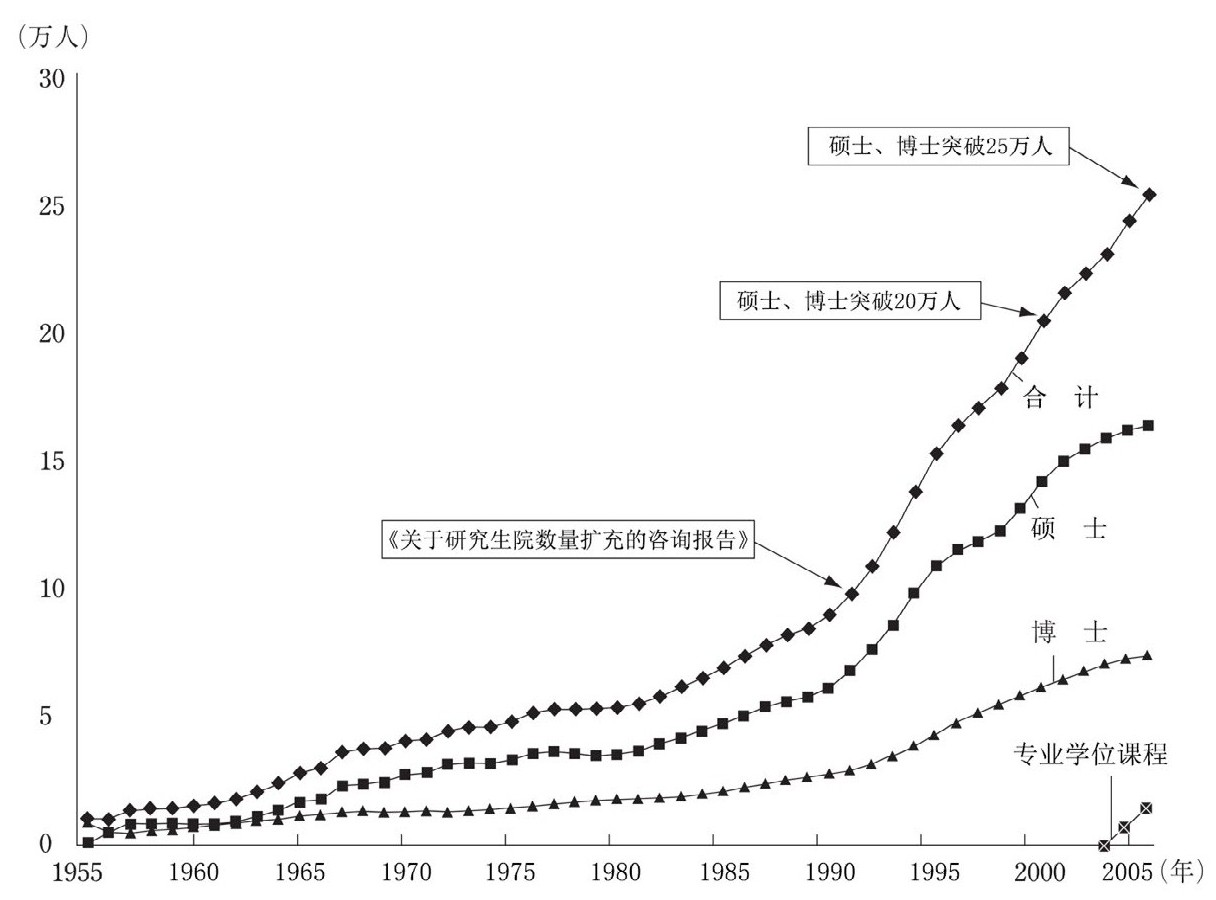
\includegraphics[width=\linewidth,keepaspectratio]{image/6-11955—2005年，日本高校硕士、博士招生情况.jpg}

\caption{1955—2005年，日本高校硕士、博士招生情况}\label{fig:6-1}

\end{figure}

\subsubsection{1. 教育资本化失控（超额扩招现象）}

倍增计划推出时，政府规划用10年时间将硕士人数增长至10万人。但实际仅5年就已经超过原定的规划扩招人数，最高峰时更是超过原定规划的2倍还多。后来超额扩招导致的研究生供给过剩，也被认为是其学历贬值的主要原因。

那么扩招为何严重超过规划？

这是因为政策放宽后大量民间资本涌入大学投资，许多不具备研究生教学能力的私立大学也开始扩招。泡沫破裂后资本将教育视为一门好生意，因为经济下行期间教育属于刚需行业。此前私立大学设立研究院的门槛极高，如今门槛放开自然导致资本纷纷涌入。

据文部省统计，4年时间里，私立大学的硕士学院数量从170家暴涨至290家。当时甚至出现学院还在筹备，但招生工作已经在开展的奇观。由于新建学院数量过快，各私立大学师资力量出现严重不足，为了争夺有限的教师资源，教育界甚至出现了所谓“一亿教授”的说法，意指私立大学邀请一位国立大学的教授，每年需要支付的报酬在一亿日元以上。

1994年私立大学报名数突破3.2万人，而当年总共只录取了2万人，这意味着即使最差的研究院都存在淘汰率。短短4年，私立大学在校人数就从不足2万跃升至4.5万人，由此可见这一轮扩张速度之快与研究生超额扩招的数量之大。

\subsubsection{2. 教育质量下滑}

除了私立大学过度扩招以外，当时还有一个严重的问题，那就是研究生教育质量的飞速下滑。由于各大学都处于扩招状态，教师数量完全跟不上硕士扩招速度。而这也导致了研究生教育质量的飞速下滑。文部省统计，扩招前全国研究院平均师生比例是1:2.7，扩招后仅三年就超过1:5。个别新成立研究生学院甚至出现一名导师同时负责10名学生的情况。

由于学生数量的急剧增加，导师们面临着前所未有的指导压力，往往只能进行一些简单的学术交流和建议，难以对学生的研究课题进行全面细致的把控。与此同时，很多学生选择读研更多是将其视为“经济冰河时期”的就业缓冲地带，而非出于对学术研究的热爱和追求。

因为毕业过于轻松，社会将研究生学院称为休闲之地，大大降低了大众对研究生，尤其是私立大学研究生的认可度。后来这段时间也被称为研究院宽松时期，意指其学历含金量明显低于大扩招以前。

至1996年日本私立大学硕士就业率跌破恐怖的60\%，成为当时所有学历段就业率最低的群体。可以说短短四年，日本私立大学硕士学历就迎来致命的贬值。

\subsection{二、扩招政策大调整，大学竞争化时期与从严考核}

1996年日本社会已经意识到过度扩招带来的危害。

{\fangsong 研究生人数增长过快，扩招后学生的综合素质出现明显下滑。—1995年《日本教育白皮书》。\par}

但面对愈演愈烈的大学生失业潮，当时日本陷入了两难的选择，如果停止硕士扩招，则原先海量的考研学生必将开始找工作，此时的就业市场根本无法容纳如此多学生。文部省统计仅1996年一年就新增22万失业大学生，而当年参加各大学硕士笔试人数高达11万，可以说考研有效缓解了当时社会恐怖的就业压力。在大扩招无法停止的背景下，日本政府于1996年提出研究生教育质量改革与博士扩招计划。一方面，政府鼓励研究生进行博士深造以延缓就业，此后又推出博士后支援计划，最高峰是在读博士数量达到7万，博士后达到1.5万，是扩招前的整整三倍。

其实日本启动博士扩招还有一个重要原因。1996年正处于“科学立国”战略最关键时期，急需海量博士人才参与到基础研究中。站在当时的决策角度思考，假设科学立国战略成功，那么大扩招的人才都可以投入新兴行业中。关于博士的情况后文再说，我们先说说日本是如何进行研究生教育质量改革的。

\subsubsection{1. 大学竞争时期——从严考核}

当时政府通过引入大学间竞争制度，将高校经费从申请制改为竞争制，企图通过竞争倒逼各大学提升学生的学术研究产出能力。此后高校间迅速形成马太效应，不具备科研能力的私立大学逐渐被市场淘汰。这一改革效果也是立竿见影，从1996年开始各大学论文总量连续3年增长超过10\%。

但对于国立大学的在校学生来说，这一改革则产生了一个巨大的问题，那就是其毕业门槛被大幅度提高，各国立大学为了竞争经费，纷纷对学生提出极为严苛的毕业论文要求。这导致许多学生无法按时完成学业，只能选择延时毕业。

根据文部省数据，质量改革前硕士的平均延毕率在8\%以下，但改革后最高达到了17\%。同时各国立大学每年还有约2000人选择退学，90年代因为考研人数众多，优质的国立大学考研竞争十分激烈，不到万不得已几乎不会有人选择退学。

可见这一轮质量改革对学生毕业难度要求之高。

\subsubsection{2. 教授的无情压榨}

但其实除了毕业难以外，当时的学生还面临一大问题，那就是教授们的无情压榨。由于日本高校采用教授负责制，教授对学院内所有学生去留问题都有一票裁定权，导致教授权力极大。

学生们想要专心进行科学研究几乎是不可能的，文部省统计1998年研究生实际科研时间仅占53\%，剩下时间都在处理非科研事项。一边是艰难的毕业论文，一边是教授的无情压榨，研究生与博士们几乎都处于严重过劳状态。

当时社会将这种畸形的导师制度称为“主公与家臣”的关系。2003年，电视剧《白色巨塔》上映。这部作品表面讲述日本医学院残酷权力等级制度，实则是影射当时各国立大学教授群体生存现状，马上引发社会热议。“本该是科研的象牙塔的大学为何沦为泯灭人性的白色巨塔”成为当时的讨论焦点。而该剧影响力之大甚至创下收视纪录，可见日本社会对这一问题的关注。

\subsection{三、“科学立国”战略失败后的就业之痛}

在竞争如此激烈环境中考上硕博，又艰难毕业的学生们，他们的就业状况究竟如何呢？让人遗憾的是，就业之痛才是这批学生们命运最残酷的考验，这也正是“研究院倍增计划”至今都在日本饱受争议的原因。

在这里，我们需要再回顾下这轮硕士扩招的历史背景，1991年当政府提出扩招政策时，是基于10年后“科学立国”战略成功，日本爆发大量新兴产业需要海量硕士与博士的人才设想。但2001年正值日本陷入最艰难的超级就业冰河时期，“科学立国”战略不仅没有成功，反而在90年代后期那场著名的芯片战争中惨遭失败。这一系列挫败导致大量扩招的人才，根本没有派上用场，就已经面临了贬值的危机。

\subsubsection{1. 隐形难民，100万余扩招的硕博学生}

“科学立国”战略失败后，日本社会不得不面对一个问题，那就是大扩招期间产生的100余万研究生与博士如何安置。这批高学历人才因年龄劣势很难在就业市场找到工作。他们究竟遭遇了什么？

\paragraph*{（1）科研机构法人化冲击}

1999年日本遭受了泡沫破裂以后的第二次经济冲击。当年因为财政负担难以维持过量的研发支出，日本启动了国立科研机构法人化改革，改革后原由政府扶持的科研机构开始自负盈亏，各大科研机构实施人员降本增效。此前各大科研机构一直是日本研究生的主要就业渠道，这轮缩招导致国立大学研究生就业率首次跌破70\%。

\paragraph*{（2）高校缩编潮}

2000年政府开始调整科研扶持政策。在前一年日本半导体市场份额被韩国超越后，基本已宣告第一次“科学立国”战略失败。此后政府宣布只对通信等四个产业进行经费扶持，放弃了此前全学科扶持的战略。2002年政府科研经费开始减少，各大高校开始缩减人员编制，由于高校与研究机构同时缩减编制，当年博士与研究生就业率双双跌破60\%，这批大龄博士与研究生被迫成为“高学历穷忙族”。

而更糟糕的是，政府于2004年宣布对高校实施经费管控改革，此后每年的高校经费都要比上年减少1\%。大量依附高校的机构被裁撤，硕博学历的失业人数进一步增加。机构裁撤潮中很多高学历者已经超过35岁，中年失业的痛苦想必今天的你我都感同身受。

\paragraph*{（3）企业支援计划失败}

2002年开始，政府启动了企业支援计划协助研究生与博士就业。政府给予一定奖励，鼓励企业雇佣研究生与博士搞研发，奖励最高时期每雇佣一名博士可以奖励企业500万日元。但现金奖励也没有换来企业的雇佣，2004年文部省调查数据显示，只有15\%的企业愿意雇佣博士与研究生。因为经过10年的经济衰退与破产潮的洗礼，多数企业都处于战略收缩阶段，对于研发创新的投入十分谨慎，因此企业没有意愿雇佣太多的研究型人才。当时正是劳务派遣最严重的时期，找不到工作的硕士博士，很多只能沦为派遣员工，与本科生甚至高中生拿着相同的薪水。而不愿从事派遣员工的高学历者，则只能返回高校从事低薪的临时教师，以期待有一天可以转正，继续干回自己热爱的科研工作。

但这一天终究没有到来。

\subsubsection{2. 就业冰河时期特别援助}

2005年为了应对经费缩减潮，日本各高校开始对临时教师制度进行改革。改革后临时教师不再有转正机会，所有合同都是一年一签，按照上课次数付费，其工资待遇与稳定性甚至低于就业市场的派遣员工。据2005年文部省统计，临时教师每节课的平均酬金在2万日元左右。为了增加课时，他们不得不同时在几所大学兼职任教。即便如此，临时教师的全年收入也往往不到全职正式教师工资的30\%，许多人甚至同时在便利店打工，过着白天在大学教书，晚上在便利店上班的生活。根据文部省2007年统计，临时教师的年收入普遍低于200万日元，属于日本的绝对贫困群体。而当时日本有整整16.8万临时教师（全教育口径），其中73\%都是35岁以下的硕士与博士生。2010年日本启动就业冰河时期特别援助，高学历的临时教师成了主要援助群体。

就此他们中的很多人挂着一纸高学历文凭，却在临时教师制度中逐渐走向贫穷。从2007年以后日本大学生开始拒绝读研考博，日本曾经稳居世界第三的科研体系走向崩塌。

\subsection{尾记：32年的轮回}

1992年，日本政府开启“研究院倍增计划”。

2002年，随着政府科研经费开始减少，这场持续了十余年的硕博大跃进画下句号。日本政府于当年宣布“研究院倍增计划”基本结束，此后各国立大学硕博人数开始逐渐回落。

“研究院倍增计划”结束后，日本政府未再对该计划发表过任何评价。直到2018年，文部省首次承认日本科研处于衰退时，才对90年代“研究院倍增计划”进行反思，90年代初对于经济复苏的过度乐观，导致未能控制好硕博扩招比例，是以后同类计划必须检讨的部分。

回望这一代扩招的硕博学生，他们一度是日本90年代最优秀的一群人，在失业潮的洪流中艰难上岸，又在高压环境下成功毕业。但个人的努力又怎能敌过时代的洪流。最终他们的命运只能随着日本经济的持续衰退走向沉沦。

2010年以后随着日本经济的恢复，企业与科研机构开始逐渐恢复对科研的投入。此后研究生就业率开始回升。但起薪基本已经与本科生保持一致。2020年以后由于经济的持续向好，日本社会开始释放大量研究生与博士招聘需求。2024年日本再次提出博士扩招计划，这一次政府希望在20年间将博士人数增长2倍。

而此时距离上一轮硕博大扩招已经过去了整整32年。

\subsection{拓展阅读}

\subsubsection{日本为何产生“博士远离”现象}

{\fangsong 自2003年“科学立国”战略失败后，日本博士人数就处于持续下跌状态。博士入学人数从2003年最高的1.8万下跌至1.4万，更糟糕的是，这1.4万人里还有43\%的在职人士与16\%的外国学生，硕士直升博士人数只有40\%，而在2003年83\%的博士都是硕士直升。\par}

{\fangsong 如今的博士课程已经沦为职场学历镀金的场所，社会普遍认为只有找不到工作的人才会去读博士，而这种现象被称为“博士離れ”（博士远离），意指博士毕业生在就业市场上长期面临就业率低于本科生的困境。而导致这一现象的原因除了“科学立国”战略失败以外，从1996年开始的博士扩招政策也在推波助澜。那么博士的政策究竟是如何演变的，又是如何导致博士远离现象？\par}

\subsubsection{1. 万博计划}

{\fangsong 1996年的“一万博后计划”是日本博士扩招的起始点，当年《科学技术基本计划》提出，为提升日本的科学研究水平，需要在2000年实现培养10000名博士后的目标。计划推出后国立大学迅速扩大了博士与博士后人才规模，最终在1999年提前完成，比原定提前一年。\par}

{\fangsong 但该计划却产生了一个严重的问题，那就是大量博士无法对口就业。由于只强调就读人数与毕业人数，各大高校在扩大招生规模的同时，并未充分考虑市场需求和就业环境的变化，将扩招重点放在了当时所谓前沿的脑科学与超级材料领域（因为同年日本推出前沿工程计划，研发总投入达到14.4万亿日元），产生了大量“無駄博士”（无用博士）。\par}

{\fangsong 许多所谓前沿领域的博士不得不接受低薪、非专业对口的职位，不仅造成了社会资源的浪费，也造成了博士的严重过剩。而同时期日本政府也忽视了对于博士就业的配套的制度以及经济支持，甚至还在其中火上浇油。1997年颁布了《大学教师任期法》，开始在大学中推广任期制，大学将退休教师的岗位回收并进行削减或重新分配的现象增多，博士留校难度也加大。\par}

{\fangsong 在这样的背景下，日本很快从“无用博士与博士过剩”向“博士就业难”的情况转变。21世纪初，日本网络出现《百名博士之村》的故事，渲染了一批博士人才的悲惨生活。\par}

{\fangsong 之后又有《高学历穷忙族》一书问世，讲述许多博士毕业生难以进入一流企业就业，甚至沦为未就业或从事非正式职业的窘境。\par}

\subsubsection{2. 财政压迫下的改革}

{\fangsong 1996年日本启动博士扩招之时，可能连政策制定者都不能预料到此后急转直下的经济环境。当第一批扩招博士生尚未毕业时，1997年亚洲金融危机便如巨浪般拍碎日本出口导向的经济支柱，连续两年GDP都出现超过1\%的负增长。至2001年小泉政府上台之时，面对庞大的赤字，内阁提出在教育界实施“没有禁区的改革”，也就是后来的大学结构改革。其中最重要的举措就是促进国立与公立大学的重组，大幅减少大学数量，而这进一步减少了招聘新教师数量。雪上加霜的是，由于当时已经进行国立科研机构独立法人改革，2001年仅三大国立研究院之一的产业技术综合研究院就裁员900人。许多原本就难以维持的科研项目和研究岗位被迫削减或取消，这使得博士毕业生就业更加艰难。\par}

{\fangsong 鉴于科研机构与大学都已经无法提供足够的就业，政府于2001年提出推动科研人才进入企业界的构想，并在此后两年推出多项政府补贴计划，而这就是“博士企业支援计划”。然而该政策的推出不仅没有降低博士的失业率，反而进一步增加了博士入学人数。\par}

{\fangsong 一方面，企业对于雇佣博士生的积极性依然不高。因为在经济形势不佳、企业自身经营压力较大的情况下，企业更倾向于招聘具有实际工作经验、能够迅速投入工作并创造价值的人员，而不是高学历但缺乏实践经验的博士生。博士生的培养成本相对较高，企业担心投入与产出不成正比，所以即使有政府补贴，企业在招聘博士生时仍然持谨慎态度。\par}

{\fangsong 然而企业支援计划在另一方面却对学生群体产生了意想不到的后果，反而吸引了更多研究生去读博士。这其中有两个原因：第一是部分学生机械地认为在企业支援计划的补贴下，博士生会比硕士生更容易找到工作；第二则是由于当时严峻的失业潮，硕士的就业率也不足65\%，很多学生认为反正也找不到满意的工作，不如进一步深造读博，一方面可以暂时避开就业压力，另一方面也期望通过提高学历在未来获得更好的就业机会。在这种思想作祟下，日本博士的入学人数在2003年达到了历史最高的1.8万人，与此同时，日本博士的就业率却也跌到了历史最低的54.4\%。\par}

\subsubsection{3. 国立大学法人化改革}

{\fangsong 而2004年政府实施国立大学法人化改革，又将博士留校就业的最后一扇门给关上。法人化改革之后，文部省对科研经费按照每年强制下降1\%的比例削减。到了后期，部分大学的人均科研经费竟低至50万日元，这般微薄的资金，几乎仅能维持电费和复印费的支出。国家对各大学的财政拨款逐渐减少的同时，大学教授的退休年龄却被延长，这导致各大学陷入了捉襟见肘的境地，鲜少有充足的经费用于招聘青年教师。在这种背景下，东京出现过300:1，甚至400:1的大学教师应聘比例，而这也是前文提到为何有如此巨量大学临时教师存在的原因。\par}

{\fangsong 最终在持续多年的低就业率与严重过剩的供应矛盾下，日本博士远离问题就此被引爆。\par}

% 逐格核对 EPUB 原图：image_009.jpg, image_010.jpg
\begingroup
\setstretch{1.25}
\small
\setlength{\tabcolsep}{4pt}
\renewcommand{\arraystretch}{1.3}
\begin{longtable}{@{}>{\raggedright\arraybackslash}m{0.31\linewidth}*{3}{>{\centering\arraybackslash}m{\dimexpr0.23\linewidth-8pt\relax}}@{}}
\caption{平成二十年（2008年），日本各学科博士主要就业率}\label{tab:6-1}\\
\toprule
\bfseries 学科 & \bfseries 毕业人数 & \bfseries 就业人数 & \bfseries 就业率\\
\midrule
\endfirsthead
\multicolumn{4}{r}{续表}\\[0.5ex]
\toprule
\bfseries 学科 & \bfseries 毕业人数 & \bfseries 就业人数 & \bfseries 就业率\\
\midrule
\endhead
\bottomrule
\endfoot
\bottomrule
\endlastfoot
人文科学 & 1358 & 418 & 30.8\%\\
社会科学 & 1238 & 526 & 42.5\%\\
理科 & 1610 & 986 & 61.2\%\\
工科 & 3636 & 2508 & 69.0\%\\
农学 & 1065 & 692 & 65.0\%\\
医学 & 5074 & 3907 & 77.0\%\\
教育 & 356 & 182 & 51.1\%\\
艺术 & 150 & 22 & 14.7\%\\
家政学 & 59 & 38 & 64.4\%\\
其他 & 1735 & 1009 & 58.2\%\\
总计 & 16281 & 10288 & 63.2\%\\
\end{longtable}
\endgroup


\clearpage
\begin{sidewaystable}[p]
\centering
\begingroup
\setstretch{1.25}
\fontsize{9}{12}\selectfont
\setlength{\tabcolsep}{3pt}
\renewcommand{\arraystretch}{1.3}

\caption{平成二十年（2008年），日本各学科博士主要就业方向}
\label{tab:6-2}

\begin{tabular}{@{}
    *{13}{
        >{\centering\arraybackslash}
        m{\dimexpr\textheight/13-6pt\relax}
    }
    @{}}

\toprule
\bfseries 学科
& \bfseries 按专业区分的毕业人数
& \bfseries 获得学位者
& \bfseries 继续深造者
& \bfseries 总就业人数
& \bfseries 从事专业技术工作
& \bfseries 研究者
& \bfseries 技术专家
& \bfseries 教职
& \bfseries 其他
& \bfseries 非专业技术工作
& \bfseries 除就业、深造以外的其他情况
& \bfseries 死亡、情况不明者\\

\midrule

合计 & 16281 & 16086 & 146 & 10288 & 9492 & 2459 & 1800 & 2564 & 2669 & 796 & 4278 & 1569\\
人文科学 & 1358 & 1348 & 10 & 418 & 358 & 24 & 4 & 274 & 56 & 60 & 589 & 341\\
社会科学 & 1238 & 1205 & 24 & 526 & 367 & 46 & 10 & 290 & 21 & 159 & 444 & 244\\
理科 & 1610 & 1583 & 26 & 986 & 898 & 427 & 295 & 142 & 34 & 88 & 483 & 115\\
工科 & 3636 & 3617 & 12 & 2508 & 2294 & 775 & 1050 & 438 & 31 & 214 & 885 & 231\\
农学 & 1065 & 1056 & 3 & 692 & 627 & 375 & 117 & 107 & 28 & 65 & 339 & 31\\
医疗 & 5074 & 5009 & 49 & 3907 & 3851 & 466 & 113 & 863 & 2409 & 56 & 855 & 263\\
教育 & 356 & 353 & 0 & 182 & 167 & 14 & 1 & 129 & 23 & 15 & 117 & 57\\
艺术 & 150 & 149 & 0 & 22 & 21 & 0 & 2 & 16 & 3 & 1 & 95 & 33\\
家政学 & 59 & 58 & 1 & 38 & 37 & 13 & 0 & 19 & 5 & 1 & 16 & 4\\
其他 & 1735 & 1708 & 21 & 1009 & 872 & 319 & 208 & 286 & 59 & 137 & 455 & 250\\

\bottomrule

\end{tabular}
\endgroup
\end{sidewaystable}

 \cleardoublepage
    % 来源：EPUB spine / EPUB/xhtml/chapter4.xhtml

\BookPart{第三篇}{就业众生相}

\BookPartImage{image/第三篇就业众生相.jpg}
 \cleardoublepage
    % 来源：EPUB spine / EPUB/xhtml/chapter4_0001.xhtml

\BookChapter{7}

\section[第七章\q 日本的全民考公热]{第七章\\ 日本的全民考公热}

\BookSubtitle{——回顾日本全民考公的30年：从狂热到寂灭}

{\fangsong 经济下行期，公务员报考人数大幅增加并非新鲜事。因为日本、韩国都在20世纪90年代经济下行期，迎来了全民考公浪潮。90年代日本青年失业率一度超过10\%，把公务员当作经济不景气的职业避风港，成为当时很多日本人的选择。\par}

{\fangsong 但回头来看，日本的考公热潮只维持了10年左右，就逐步消退。\par}

{\fangsong 2023年日本公务员报考录取比例已经降为1:3，录取难度创下30年来新低。现阶段日本公务员的录取难度已经降低到与中小企业相等。\par}

{\fangsong 日本的考公热是如何升起又落下的呢？\par}

在日本雅虎网站上有一个热帖“在泡沫时代，选择公务员是不是很不寻常”。对于那些泡沫时期参加工作的60后来说，他们通常在帖子里表达的是自己因为不够优秀，所以才成为公务员的庆幸。80年代，只有不够优秀的学生才会从事公务员工作几乎成为共识，因为枯燥且稳定的工作完全不符合泡沫时期的暴富狂热，由于录取门槛极低，当时的市政厅被称为高中学历的乐园。

但当泡沫破裂失业潮来袭后，公务员因为稳定的特性被捧上神坛，大学生们将其称为神的职业。1995年日本公务员报考人数总计达到65万，是泡沫时期的两倍还多，几乎与当年高中学历以上毕业的人数持平。无论是本科生、研究生还是博士生，他们毕业后的第一件事就是备考公务员，就连日本第一学府东京大学的毕业生，也以成为一名公务员为荣。

而2024年，日本公务员报考率甚至低于泡沫经济时期。让我们从泡沫年代开始，逐一回顾这场考公浪潮。

\subsection{一、泡沫年代，成为公务员=人生失败组}

泡沫经济时期，成为公务员，尤其是地方公务员的名校大学生通常被称为“負け組”，也就是“人生失败组”的意思。

1988年NHK舆论调查所进行了一次大学生就业调查，充分表达了这种公务员遇冷的现状。结果显示80\%大学生表示希望去民间企业工作，只有16\%的学生表示想去政府机关工作。也就是说四分之三的大学生都不想成为一名吃财政饭的人。

而另一项更有趣的数据是，超过7成的大学生都想去大都市工作，希望回到家乡就业的只有30\%，而其中绝大多数还是女性。彼时大都市的银行证券公司或者大型商社工作才是就业最好的选择。1989年日本最受欢迎的职业与公司选择中，有3家银行与2家地产公司，公务员已经连续10年未能进入前十之列（最后一次出现已经要追溯到1980年）。

造成这种现象的重要原因是当时巨大的“公私薪酬差异问题”，简单来说就是民间企业无论是在薪资待遇还是福利上，都要比待在政府做一名领着微薄固定薪水的公务员好得太多了。

自1960年代，日本实施国民收入倍增计划以后，民间企业纷纷提高薪酬，再加上70年代后，日本在出口领域取得了卓越的成功，这些大商社每年都会为职员发放丰厚的年终奖。

经济腾飞时期，公务员与民间职员的待遇被迅速拉开，虽然从基本工资上看，80年代公务员工资与民间企业职员相差不大，但在那个年代谁会在乎自己的基本工资？年终奖才是收入的最大部分。

当时日本企业通常实行的是双份年终奖制度，也就是夏季奖金与冬季奖金。通常企业会根据当年的经营情况发放奖金，这也被视为日本企业“家文化”的重要表现：艰难的时候，大家一起扛；成功的时候，自然大家一起分享成果。

而80年代日企的成功有目共睹，奖金的数字自然也水涨船高。当时奖金的发放标准被形象地称为“246”，也就是绩效最差或者刚入职的员工可以拿到一年200万奖金，普通员工则是400万，优秀员工则可以拿到600万。

这还只是中等企业的标准！大手企业则更加慷慨，日本股市上涨最快的80年代后期，每年四大证券公司（野村、大和、日光和山一）的年终奖都会成为社会热议的话题，盛传野村证券的中层干部可以有超亿元的奖金。而同样作为当年大热的房地产行业，发起奖金也毫不手软，1989年西武集团普通职员的平均年终奖达到500万日元，中层干部基本能达到千万级，稳坐日本房地产企业第一。而丰厚的年终奖也让从业者可以实现“一万日元打出租车，十万日元喝酒”的美好生活（注：按1989年日元汇率，10万日元约合12000元人民币）。

除了双份年终奖以外，正式社员还可以享受带薪出国度假旅行等福利，只要是大一点的公司都会与旅游酒店签署长期的包房协议，以方便社员在度假期间免费入驻。早年播出的《蜡笔小新》动画片中，就有许多野原广志享受到公司免费的度假酒店福利的剧情。但有趣的是，随着时间的推移，后来的《蜡笔小新》动画就逐渐减少了这种设定，取而代之的则是美伢预定各种廉价酒店的故事，这也深刻反映了日本民间企业对于员工福利的变化。

那么当时日本公务员可以带来什么？在工资方面虽然从1973年开始，日本人事院就提出增加公务员待遇，但到了1989年日本地方公务员的普遍薪酬还只有500万日元（含奖金），与民间企业算上年终奖后的待遇，存在着巨大的差异。

而国家公务员虽然略高一些，能够达到600万日元，但要知道能成为国家公务员的可都是来自顶级名校的精英。而在泡沫经济时期，顶尖名校学生就是被全社会企业热捧的存在，又怎么会看上这一点点薪酬。

80年代，为了争夺名校学生，社会逐渐衍生出了一种“买青田制度”，也就是通过付给名校大学生一笔巨额“青田费”，要求他们在毕业后一定要来其公司工作。80年代后期，顶尖大学生的青田费普遍在300万日元左右，如果是东京与京都两所大学的毕业生甚至会赠送高级轿车。除此之外，个别企业甚至还会向他们承诺在入职后给予特定的职位晋升，这在采用年功序列制的日本是难以想象的。而除了学生本人，学生的父母也是企业攻略的对象，如果大学生来自乡下，企业往往会送给父母一头牛以表心意。而如果大学生来自城市，企业则会送给其父母一套高档的高尔夫球具与化妆品。如果是银行，甚至还会向下属公司提供更加优惠的贷款，以招聘到他们职员的孩子。可见“买青之风”的疯狂。

在这种狂热的氛围下，不要说东京与京都这两所日本TOP2院校，就是旧帝国七大\footnote{旧帝国大学，即日本在明治维新时期到第二次世界大战结束期间的“大日本帝国”时代设立的大学。七所帝国大学为：东京大学、京都大学、东北大学、大阪大学、名古屋大学、九州大学、北海道大学。}的另外5家，毕业三年内年薪达到千万都并非难事。

更令人忍俊不禁的是，80年代日本公务员普遍还采取的是非双休制度，也就是一周只能休息一天，而82\%的民间企业已经实施双休制度。

外面的薪酬如此之高，福利如此之好，试问有哪个大学生会看得上这个工资又低，休息时间又少的工作？此时名校大学生择业第一优先志愿是银行，第二志愿则是证券公司，第三志愿是大型商社，即使是霞关的中央机关公务员都排不进前三，更不要说那些不入流的地方公务员。

80年代后期，三大核心都市的公务员报名人数还能达到岗位的五六倍左右，但中小城市的地方公务员报名数通常在1:3以下，如果是偏远地区则经常发生零报名的记录。这导致部分乡村不得不为了填补人手，将公务员入职门槛下调到高中。但你以为这已经是最差的情况了吗？

泡沫时期，过于危险与劳累的公务员岗位被称为“3K岗”，这些岗位根本就不会有年轻人愿意报考，其中典型的3K岗就是陆上自卫队、警察与消防员，这些岗位只要报名就可以保证100\%录取。当时甚至有玩笑说，在报考陆上自卫队时，笔试考官会指着试卷上的错误答案说：“要不重新看看？”

但令人唏嘘的是，90年代3K岗因为招聘人数众多，考中的成功率高，成为大学生追捧的对象，尤其是警察岗位因为有额外的执勤补贴，报考人数一路走高，当然这就是后话了。

在经济最疯狂的1989年，国家公务员考试人数只有2.7万人，占当年大学生总数不到5\%，而在12年前的1977年，当年国家公务员报名人数是5.2万人。这意味着日本在这12年间大学毕业生人数增长了一半，但考国家公务员的人数却下跌了一半，而这还只是国家公务员的情况，地方公务员报考意愿只能更低。

可以说优质人才几乎全部流向了企业，只有去不了大公司的学生才会成为公务员。更糟糕的是当时还有大量在职公务人员蠢蠢欲动，由于外面的工资实在太高了，从1985年至1989年，日本国家公务员离职数量增长了近2倍。

由于报考人数实在太低，同时大量公职人员被大企业薪酬吸引，选择辞职下海，1989年日本人事院不得不临时增加公务员待遇，当年所有公务员临时加薪3\%，而对新入职的大学生则加到了4.3\%，仅此一项每年就为财政增加了3300亿支出。

但这样的加薪幅度反而在当时引发了巨大的嘲笑，毕竟泡沫时期每年涨薪10\%都被认为是工作出了问题的处罚，更何况这不到5\%的涨幅。

当时如果你从名牌大学毕业，成为一名公务员，是会被同学们嘲笑为无法进入大手企业的失败者。

但很快他们就笑不出来了。

\subsection{二、全民考公时代到来——地方公务员的美梦}

随着20世纪90年代日本泡沫经济破灭，大量的企业倒闭，日本年轻人失业率空前高涨。1991年世界市值第一的证券公司野村证券宣布冻结招聘，同时地产的暴跌导致房地产企业进入破产倒闭潮。这时候别说招聘大学生了，老员工不失业已经是万幸了。

泡沫经济时期，日本金融地产行业是全社会盈利最多、产生富豪最多、工资最高的超优质行业，海量社会精英涌向金融行业，当时这两个行业的总从业人数接近1000万人，相当于全国总劳动人口的六分之一。而伴随着这两个行业的暴雷，失业潮也随之而来。

以商科为例，在80年代的泡沫经济时期，商科毕业生是日本社会当之无愧的精英象征。前所未有的经济繁荣与地产红利叠加，使得商科专业成为无数年轻人梦寐以求的选择，但到了1995年即使是顶尖大学的毕业生，其就业率也只有72\%。要知道商科可是日本80年代扩招最为迅猛的专业之一，可以说他们以最高的分数线被录取，但在毕业时却迎来了最差的行情。

在这样的背景下，人们终于开始逐渐注意公务员这个已经被忽视了10年的选择，无论是大学生还是在职人士终于意识到永不失业的岗位是有多弥足珍贵。

从1991年开始，日本公务员报考人数开始一路水涨船高。在日本社会就业最困难的1998年，亚洲金融危机冲击导致市场岗位锐减，当年64\%的应届大学生都参与了公务员考试，录取难度一路飙升，个别优质岗位的录取率不到3\%。当时就连在婚恋市场上，一句“我在考公务员”，也会给异性留下积极向上的好印象。

但你以为稳定才是全民考公的原因吗？

其实高工资才是当时公务员受追捧的原因。泡沫破裂后的前三年，日本政府采取大规模经济刺激政策，新增国债进行公共工程投资以刺激经济，即所谓的大基建。1992年至1995年间，日本政府总计实施了6次大基建计划，新增超过40万亿基建项目，基建支出一度占到财政总支出的23\%。

通过超发债务的大基建的刺激，地方政府的财政收入被大大充实。部分地区政府收入甚至超过了泡沫破裂前的水平。在此背景下，各地政府纷纷提高当地公务员的工资。由于此前政府机关已经多次跟随泡沫时期加薪，再加上日本公务员是年功序列制度，每年还有额外的固定加薪比例，这使得个别富裕地方的公务员工资爆炸式提升。以1995年横滨市公共交通部门为例，其公车司机平均收入接近900万日元，高出当时同年限社会平均工资的30\%—50\%。

更加讽刺的是，大基建的巨额收入导致各地形成了庞大的利益党团，由此形成了90年代早期，日本中央公务员最穷，地方公务员最富的收入倒挂现象。而在庞大的基建投资刺激下，各地出现了类似“县城婆罗门”的说法，他们称之为“农林公建党团”，大量依附在基建产业链上的地方公务员赚得盆满钵满，在利益刺激下，日本许多名校学生扎堆报考地方公务员。

短短十年，日本就从大手企业年薪千万，变成了地方考公年薪千万。

可以说日本在泡沫破裂后的前5年，公务员系统度过了一段相当平稳且美好的时光。虽然可能加班较多，但相比较其他工作绝对是一个好选择。而在惯性思维的作用下，很多日本公务员都认为这种稳定还将保持一段很长的时间，甚至是一辈子。由于地方政府大幅度提高公务员收入，同时日本失业率逐年升高，公务员高薪稳定优势开始体现。日本在1994年以后，公务员报考人数快速增长，每年的报考人数增长超过20\%，竞争最激烈的时候，大学生需要从大一就开始准备公务员考试。

但你不要忘了，这一切的美好与稳定都是建立在什么之上！

\subsection{三、日本第一次财政改革的冲击——外包改革}

虽然日本公务员的日子好过了，但财政的日子却越来越难过了。由于长期的举债，中央政府赤字自1992年后逐年扩大，大规模的基建支出使得本就艰难的财政更加恶化。

1996年日本未偿国债为244万亿，占GDP的比例接近一半，基建刺激政策难以维系。自此，日本被迫进行了泡沫后的第一轮财政改革。时任内阁在1996年下半年提出了开源节流的财政改革，要求各地政府大幅降低政府支出。

但这一次开源节流的影响其实并没有传导到公务员体系。

当时日本降低政府支出的重点放在了清理派遣员工上，即所谓解雇非正式员工。日本政府采用了外包与清理两条思路，一方面将城市基础维护工作交由第三方私企处理，降低基础设施维护人员数量，美其名曰将民间的事情重新交给民间企业来做。另一方面则是解雇大量的临时员工。

根据日本经济新闻1997年的抽样统计，90个样本单位，其临时工平均解雇比例超过40\%，有67家单位都进行了业务外包以降低政府支出。换句话说，日本公务员改革的第一刀砍向了临时工体系。但由于第一次改革基本没有触及所谓编制内员工的利益，日本编制内公务员高薪依然得以保持。

90年代中期，日本公务员有了一个“1000万人生胜利组”的外号，即当时发达地方公务员普遍年收入均能超过1000万日元，超过了丰田等头部企业的员工平均工资。

对临时工体系的改革，反而进一步刺激民众报考正式公务员的热情。根据《日本经济新闻》1997年报道，日本最高学府东京大学，一天举办了超过30场的公务员培训。从最高学府到普通大学，日本毕业生的第一选择似乎都变成了考公务员。

当时所有人都相信公务员就是神的职业，所有大学生都把考公务员当成人生第一要义。

但这一切却在1998年发生了改变。

\subsection{四、日本第二次财政改革的冲击——降薪缩编潮}

我们已经说完了第一轮公务员改革的情况。那么到了1998年以后的日本公务员改革是怎么样的？1998年是日本公务员体系改革的一个分水岭，如果说此前的改革基本是修修补补，那么之后的改革则是真正意义上的大刀阔斧。

首先1998年日本遇上的最大问题就是亚洲金融危机。当年日本中小企业与银行陷入倒闭潮，日本政府不得不再次启动刺激政策。1998年桥本内阁决定暂缓财政改革，推出了16万亿元的刺激政策，但难以修复下行的经济形势。当年又再次出台24万亿元的紧急刺激计划。

1998年这一轮经济刺激计划无论是频率还是金额都超过了泡沫破裂后第一次经济刺激计划。但这一次日本政府不再以基础建设为刺激手段，而是更多围绕中小企业纾困，刺激思路从保经济增长转为保企业生存。因为日本政府已经意识到通过基建已经很难拯救经济了，政府急需将经济刺激思路从投资拉动转为企业增长。

在经济刺激思路调整的大背景下，日本大基建投入开始大幅度萎缩，从1998年开始连续7年基建投入均为负增长，2004年基础建设投入已经低于1981年水平。由于日本地方政府基本是靠大基建的大量资金维持地方政府运转体系，而大基建资金的突然抽离，让日本许多地方政府瞬间陷入财政危机。

90年代初还是人生胜利组的地方公务员，瞬间就陷入了工资发不出的困境。

而1998年也成了无数日本公务员人生的分水岭。

屋漏偏逢连夜雨，日本政府在1999年后启动了第二轮财政改革，直接指向日本现行公务员体系。由于公务员长期占用大量财政预算但产出明显偏低，再加上当时社会对于公务员的尸位素餐多有怨言，90年代后期，人事厅开始加强了公务员的各项考核。1997年政府设立公务员制度调查会，提出能力与业绩导向的晋升和薪酬制度。2001年，内阁官房行政改革推进室发布年轻公务员的调查结果，揭示现行制度的问题，提出需要加强对公务员尤其是年轻公务员的管理工作。

在此背景下公务员工作强度被不断加大，根据人事院的数据，2000年后，日本每月加班时长超过100小时的公务员占比9.1\%，每月加班时间超过80小时的占比30\%。作为公务员核心的霞关则被称为一座永不下班的“不夜城”，凌晨三四点钟才回家的大有人在。日本公务员也就是从此时开始从“帝国精英”变成“霞关的抹布”。

但你以为这就结束了吗？1998年中央公务员限额改革启动，当年自民党联合政权成立，同意削减25\%的国家公务员，并在1999年废除政府委员制度，引入副大臣和政务官制度。2000年森喜朗内阁的行政改革大纲提出广泛改革，继任的小泉纯一郎内阁以“无改革无增长”为口号推进改革。此后，安倍晋三成立内阁人事局，日本长期公务员限额制度持续推进。

如今日本已经成为全世界发达经济体中“官民比例”最低的国家，据日经中文网在2021年的统计，每1000人中，日本有公职人员37人，而法国有90人，美国差不多是64人。日本公职人员占比只有法国的四成，美国的六成。对于日本的老百姓来说，这意味着财政供养人员少，是件好事。但对于日本的公务员群体来说，这只意味着一件事，那就是人少活多，非常累！

但工作压力增加并不是这场改革的终点。1999年开始，日本内阁连续五年削减国家公务员工资，以2003年为例，全日本公务员平均工资减少了16.3万日元。根据历年国家公务员工资建议书统计，公务员工资降幅总计超过40\%。

可以说1999年开始的薪酬体系改革，完成了对日本公务员体系的最后一击。2023年日本地方公务员平均年工资已回落到470万日元，仅为90年代最高峰的50\%。要知道中央公务员在日本一直是顶级名校的自留地，以往门槛相对较低的地方公务员才是普通人最主要的选择方向。但由于1999年财政改革的持续影响，日本地方公务员此后20年保持了低薪且内卷的状态，一方面大基建停止，地方财政困难人员编制不断减少。另一方面此前日本大基建债务导致地方政府难以支付公务员工资。

就此日本公务员报考人数开始下降，全民考公现象开始退烧。

\subsection{五、新世代，不考公务员}

2024年日本地方公务员报名人数仅有4.7万人，同比2023年又下降了7.2\%，35个地区的报名比例已经不足1:3。而国家公务员考试一般岗位的报考人数更是下跌至2.42万人，同比减少7.9\%，创下12年以来的新低。根据日本总务省资料，日本国家公务员综合职岗位录取比例为1:7.5，相当于每8个人录取一个人。在日本47个省级（都道府县）政府中，有45个反映没有完成招聘计划。与其他竞争激烈的亚洲国家相比，想要在日本当上公务员可谓轻而易举。

而对于社会精英来说，公务员更是成为性价比非常低的工作。2012年至2022年，入职日本中央政府（霞关）的东京大学毕业生减少了60\%。同时随着日本经济的恢复，民间企业与公务员薪酬待遇再次被拉大。一个有趣的例子是，2022年日本金融厅开出1000万日元的年薪，和企业争抢IT人才，而同类型的岗位在大手企业是2000万日元以上。

2020年后，日本连续3次上调公务员待遇，只是新世代已经无人报考公务员了。

本章我们回顾了日本考公热的起与落，那么作为人们眼中最为稳定的“医师公”群体的另外两个，教师与医生在泡沫破裂后的职业环境是如何的？我们将在未来两章讲述。
 \cleardoublepage
    % 来源：EPUB spine / EPUB/xhtml/chapter4_0002.xhtml

\BookChapter{8}

\section[第八章\q 少子化与教师过剩危机]{第八章\\ 少子化与教师过剩危机}

\BookSubtitle{——回顾日本教师改革史：未来教师还是好选择吗}

{\fangsong 20世纪80年代，教师是日本最受人尊敬的职业，是与律师医生一样被称为先生的职业。\par}

{\fangsong 但在90年代财政紧缩与少子化问题的持续冲击下，日本政府面临巨大的财政压力，不得不启动平成教师改革。改革后教育经费被大幅削减，虽然缓解了财政压力，但也让教师的工作强度与淘汰压力大幅升高。如今在日本，教师被称为黑色职业，是过劳死最严重的行业，也是大学生最不愿意从事的职业之一，2024年的报考比例不足1:3。\par}

{\fangsong 回望这一代教师群体，他们曾经是社会最受人尊重的一群人，但却在人口暴跌与财政危机中，变成了所谓的财政负担，最终在一次又一次的改革中，成为泡沫崩溃后的牺牲品。\par}

{\fangsong 那么这一切是如何发生的？\par}

2020年，“\#老师快死了（先生死ぬかも）”这个话题在日本推特上爆火，相关的推文超过一万条，无数中小学教师在推特上抱怨自己已经快被工作压垮了。由于引发的社会讨论过于巨大，TBS电视台还为此进入一所小学跟拍，完整记录了一名老师从早上7点到凌晨1点的日常工作，纪录片中展现的极高的工作强度，又一次震惊了日本社会。

这已经不是第一次出现群体性的教师抱怨问题，自2007年厚生劳动省首次就教师工作环境发布专项报告以来，“教师过劳”这个话题在日本已经被热议了快20年。

如今教师在日本社会被称为黑色职业，是过劳死最严重的行业，2023年其平均报考录取率更是不足一比三。80年代，教师曾经是最受大学生欢迎的职业之一，但在2024年已经连续多年排在日本大学生最不愿从事的职业之列。

而这一切都要追溯到90年代的那场改革。

\subsection{一、第三次婴儿潮的教师扩招}

“第三次婴儿潮”指的是原本应该发生在20世纪90年代的日本出生人口高峰。80年代初期，厚生省预计70年代近2000万出生人口，将在90年代生育1600万新生儿。为避免70年代各项资源紧缺问题重演，于是政府在1985年提出第三次婴儿潮对策，其中增加教师数量是主要措施之一，这就是昭和六十年（1985年）教师增员计划。

1985年，日本总计招聘了3.8万名教师，此后连续5年的招募人数都超过3万人，要知道这一教师增员是建立在70年代教师已经大扩招的基础上。至1991年，全国小学、初中与高中老师加总达到了惊人的105万人，创下历史新高。

但今天的我们都知道，第三次婴儿潮并没有到来，但巨量的教师却给财政体系背上了沉重的经费负担，可以说正是对这轮婴儿潮的严重误判，给日本此后20年的教师改革埋下了伏笔。关于改革内容我们稍后再说。

虽然回头看这些政策有些匪夷所思，但在当时几乎所有人都觉得应对第三次婴儿潮的计划十分必要。中曾根康弘与竹下登前后两任首相都向民众保证，政府已经为第三次婴儿潮做出了充分的准备，请大家无需担心。

那么全社会为什么会对第三次婴儿潮如临大敌，实在是因为过去两次婴儿潮对社会的冲击过于剧烈。

二战结束后，日本曾经出现过两次婴儿潮的冲击。第一次是1945年到1955年的团块世代冲击。50年代日本妇女平均生育5.2个孩子，1949年出生人口达到270万，创下日本有出生人口统计以来的最高值。而当60年代末期这些团块世代结婚生子后，带来的则是1970年至1980年的整整10年第二次生育高峰，也就是团块次代冲击。

而这两次婴儿潮分别给社会留下了“住房紧缺”与“教师紧缺”两大社会记忆。

1950年第一次婴儿潮时期，日本出现了大面积住房紧张问题，10年新增2200万人，相当于总人口数涨了30\%。政府不得不新建大批量团地住宅（造型类似于筒子楼），这些团地住宅甚至无法做到食宿分离，除了造价便宜几乎没有生活品质可言，而就是这样的筒子楼还是当时中产阶级才能购买的住房。如果是普通工薪阶层，一家数口就只能挤在简易木房中，当时这些木房社区绵延数公里，几乎与贫民区无异。1952年日本发生举世震惊的“鸟取县大火”，全市70\%的建筑被烧毁，罪魁祸首就是绵延6公里的木制平房。

第二次婴儿潮时期，日本则出现了大面积的教师紧缺问题。60年代中后期，由于二战后首批扩招教师逐步到达退休年龄，日本教师数量进入下降周期，以小学为例，1964年日本所有小学教师总数首次跌破30万。但与教师数量减少对应的却是学生数量的暴涨，1970年日本全国小学在校人数是800万，此后一路上涨，到1982年突破1200万大关。

虽然60年代末期日本加大了教师的培养力度，但最高峰时小学教师与学生比依然一度接近1:40，而初高中的教师因为培养周期更长，所以更加稀缺。由于申请人数众多但教育资源有限，所有的高中、初中、小学甚至幼儿园都以入学考试来筛选掉大部分申请者，彼时好学校招生名额30倍或者40倍的申请数是十分常见，几乎不存在不需要考试就能读的学校。

再加上家长普遍是50年代通过读书从乡村走向城市的一代人，作为文凭改变命运的受益者，他们更是把学历视为都市生存的首要法则，为了孩子上榜用尽一切手段。70年代，初高中的入学名额是绝对的政治硬通货与资源交换工具，部分校长甚至会为一个入学名额收取2—3个家庭的礼物，家长们即使知道成功希望渺茫，但为了一点点入学的可能性也趋之若鹜。

在这种教育资源极度稀缺的背景下，日本社会也常常将70年代称为“教员不足年代”。70年代中后期由于学历竞争问题过于严重，政府不得不在1976年推出《新教育课程基准》要求为学生减负。但法案推出后由于担心公立学校减负导致孩子学力下降，反而促进了日本私立中小学进一步兴起，如今私立中学已经成为日本顶尖大学的绝对生源群体。

由于这段记忆对于民众过于深刻，因此当第三次婴儿潮到来之前，几乎全社会都在认为扩招教师是必要的，必须防止第二次婴儿潮时期严重的教师不足问题重演。

但这轮婴儿潮真的来了吗？

\subsection{二、消失的婴儿潮}

1985年第三次婴儿潮应对计划公布，社会普遍预测90年代的每年出生人口在160万左右。但1992年日本总共只出生了121万人，而这已经是90年代的最高峰了。据统计，90年代全国仅出生了1100万人，比预期整整少了500万人。

新生儿的断崖式下跌，使得大量新建的妇产医院与学校迎来闲置。幼儿园成了最先受到打击的对象，90年代中期，仅东京一地每年倒闭的幼儿园数量就在30—50家左右。在老龄化加速的10年间，妇产科却成了医院里最清闲的科室。尽管日本在1995年紧急实施了“天使计划”与“紧急保育”两大刺激生育政策，但依然未能扭转颓势。

从社会演变趋势看，第三次婴儿潮的消失对社会的影响极为深远，由于日本就此失去了每25年一次的人口生育周期，人口彻底进入长期下行的踩踏下行螺旋。2015年本应是80年代日本政府规划的第四次婴儿潮起点，但也就是在这一年新出生人口首次跌破100万大关。在第三次婴儿潮消失的15年后，日本人口总量首次进入负增长状态。而人口红利的消失也让日本制造业和科研产业失去了生力军，从而深远改变了国家经济的长期发展趋势。90年代各项政策不得不面临紧急调整，而教育系统就是其中调整幅度最大的一环。

可以说，这轮婴儿潮的消失打了政府与社会一个措手不及。

整个80年代，厚生省甚至没有把“人口减少”作为社会性问题进行讨论，就连“少子化危机”这个词都要等到1992年才在人口白皮书中正式提出。因为受到两次婴儿潮的影响，日本专家基本认为人口减少都只是暂时性的，民众非常确信每隔20—30年日本就会有一次婴儿潮，“人口过剩警戒理论”在日本社会长期占据主流地位。

80年代房地产价格之所以如此疯狂，也与当时盛行的第三次婴儿潮后，日本人多地少情况将更加严峻的认知有关。

但少子化的问题并非没有先兆，80年代经济欠发达地区其实已经感受到寒意。1985年以后，岩手县与秋田县这些远离三大都市圈的偏远地区，以及完全以资源开发为导向的城市，因为经济落后首先出现了人口外迁与生育率下滑。

但政府没有对这一现象予以重视，反而还将其归咎于地方经济发展问题差异。当时任岩手县知事的增田宽在全国知事大会提出“少子化问题应对议案”之时，反而被其他县区官员指责是危言耸听。相比较少子化问题，80年代各地政府更加关注的是老龄化问题。从政府到民间，至少在泡沫破裂以前，都不认为日本将迎来出生人口暴跌的风险，而从后来的发展来看，这些经济欠发达地区官员的人口警告并非危言耸听。2024年岩手县和冲绳县已经成为日本少子化最严重的两个城市，预计到2050年两市人口将比1995年最顶峰时减少约50\%。

作为日本最早提出少子化危机的人，如今已经成为人口问题专家的增田宽回忆这段往事时评价：全社会对于人口增长趋势的严重误判，导致80年代没有及时采取措施提前刺激生育率，到90年代新生儿开始暴跌才幡然醒悟。

90年代之所以会有如此严重的生育断崖，主要有两个因素。第一个自然是大家熟知的经济衰退，因为收入下降再加上失业潮，年轻人生育意愿大幅降低。但还有一个更加隐形的原因，那就是日本政府长期实施的限制生育政策的负面刺激。

1974年为了遏制人口过剩问题，人口事务委员会推出“两孩宣言”半强制要求每个家庭只生两个孩子。法案推出第二年，新生儿跌破200万大关，到了1980年全国新生儿数量只剩下158万人，创下二战后最低值。

事后来看，如果在1980年第二次婴儿潮结束的时点就停止“二孩宣言”政策，日本人口长期稳定增长的大趋势还不会受到重大影响。但长期“人口过剩理论”的观点影响下，该项政策又被延续了整整10年。1989年日本总和生育率跌破1.57，创下有史以来的新低，全社会爆发著名的“1.57人口冲击”讨论，年底日本泡沫经济也走到终点。

泡沫经济破裂是人口下跌的表面因素，但长期错误的人口政策才是导致少子化危机的真正元凶。

那么面对消失的婴儿潮，日本政府的教育体系将面对哪些冲击？

\subsection{三、泡沫后的财政冲击}

1990年由于地产泡沫破裂带来的经济衰退冲击，日本财政体系开始迅速恶化，至1992年社会迎来泡沫后首次财政赤字。虽然政府采取了扩张性的政策措施，扩大国债发行增加收入，但举债的资金绝大多数都投向了大基础建设领域，因为这可以快速带动就业。整个90年代，全国每年的财政性投融资金额都保持在40万亿—50万亿日元，至1998年政府性质固定资产居然占到GDP的6.2\%，是欧美同期的3.1倍。

有限的资金都投向了大基建领域，那么压缩其他领域的资金就是必然的情况，而教育经费就是其中主要的削减对象。

经过80年代连续的教师大扩招与新建校园，教育经费占比从1985年开始持续攀升，至1991年教育经费已经占政府总支出的五分之一。由于过去40年日本采取的都是教育薪酬国库支付制度，教师工资的三分之二都由国家财政承担，这给中央政府造成了巨大的压力。

随着经费削减，一个严峻的问题摆在政府面前，那就是当教育经费大幅缩减后，如何才能供养庞大的教师队伍。经历过70年代与80年代的两轮教师大扩招，全国容纳了100万中小学教师。但消失的第三次婴儿潮却让这批教师没有了用武之地。

一边是学生的不断减少，一边是教育经费的不断缩减，最终政府于90年代启动一系列中小学教师改革以缓解财政紧缺与教师过剩的压力，而这就是在日本教育界备受争议的平成教师大改革。

改革后，教育经费10年间缩减近5成，虽然大大缓解了财政压力，但也让教师的工作强度与淘汰压力大幅升高，让如今的日本教师成为过劳死最严重的黑色职业。

那么当年的日本究竟是如何进行这场改革，教师群体又受到了哪些影响？

\subsection{四、教师大缩招（1992年至1995年）}

1992年文部省启动了泡沫后第一轮教师改革，而这也成了平成教师改革的开始。为了应对严重的教育资源冗余问题，减少新教师数量成了这次改革的核心。

至1995年，全国招聘教师数量相比较1989年已经缩减近60\%。据统计整个80年代日本总计招聘了42万名教师，而90年代只招聘18万名。以受影响最大的小学教师为例，1991年全国招聘小学教师还有1.5万名，到了1995年就已经减少到5700名。

那么为何这轮缩招如此剧烈？其实除了降低财政支出以外，最主要的原因还是化解第三次婴儿潮扩招所形成的教师严重过剩问题。

1992年，第二次婴儿潮的学生已经基本从中小学毕业，最晚到1998年最后一批婴儿潮的孩子都将完成自己的高中学业。从数据来看，1986年全国小学人数为1100万人，到1995年就只剩下可怜的680万人。虽然学生人数大幅减少了，但这10年间教师规模却几乎没有发生变化。要知道这批教师都是泡沫经济时期扩招的“高薪教师”。当时为了招聘到大学生，各地纷纷祭出高福利政策，但到了90年代，这就成了巨大的过剩的负担。当时教师属于国家公务员序列根本无法裁撤，因此只能选择先减少新教师数量。

但缩编必然产生一个严重的问题，那就是大量教育专业学生无处就业。1995年全国教育学院就业率仅有50\%，成为当时就业率最低的专业。教育本身就业渠道就十分单一，一旦未能成为教师就很难在就业市场找到工作。

据厚生劳动省统计，整个90年代全日本有100万教育资格证持有者未能成为教师，其中大多数都是教育相关专业。后来这一问题也被称为冰河时期教师就业困境。由于教育背景与文科十分相似，此后未能就业的他们又与文科专业毕业生在就业市场争夺本就稀缺的文科岗位，最终导致教师就业困境逐步演变成90年代的文科就业困境。教育专业的学生们成了第一轮改革的牺牲品，或者说是日本少子化浪潮下的牺牲品。

那么牺牲如此巨大的情况下，这轮改革就此结束了吗？

\subsection{五、教育市场化改革（1996年至1998年）}

1996年通过多年的大缩招，日本教育支出开始回落，当年占政府开支比例首次回落到12\%以内。笔者要强调，虽然教育支出减少，但财政赤字却更加严重了。这是因为泡沫破裂后社会失业率飙升，政府被迫启动大基建计划，创造海量就业以缓解失业潮，而这又产生了新的财政赤字。

面对这一财政困局，此后政府选择继续加大基建投入，这导致财政被进一步压缩，而教育再次成为压缩方向。而这也促成了泡沫后日本第二次教师改革。1996年底，日本启动了第二次教师改革，当年政府提出经济利益至上的教师市场化改革，此后义务教育由公益化向市场化转变。而在这轮市场化改革中，推广临时教师制度与扩大教师工作范围成为重点方向。

\subsubsection{1. 临时教师制度改革}

当时庞大的编制内教师给财政造成巨大的负担，每年仅工资一项国库支出就高达三万亿。由此政府提出需要对教师编制实施只出不进的总量控制，此后新增教师基本以合同制的临时教师为主。根据文部省数据，改革后临时教师数量增长近5倍，最高峰时占到全国教师总量的六分之一。

而通过该制度，正式教师数量被有序压缩，此后5年正式教师数量被缩减近7万人。但这轮改革又给学生们造成了巨大的伤害。由于新增教师编制被严格管控，成为正式教师极为困难，甚至需要国会议员进行推荐。在此背景下，多数教育专业毕业生被迫成为临时教师。但要知道临时教师合同一年一签极不稳定，收入也仅有正式教师的一半，这给后来的社会造成了十分严重的临时教师贫困问题。但在当时，由于社会正处于失业潮期间，即使是没有编制的临时教师，也让无数名校学生趋之若鹜。

《日本经济新闻》报道，2000年东京地区的临时教师报名录取比例甚至低于9\%。而其中大多是在缩编潮中没有找到工作的教育专业学生。

可以说大缩招后的学生们再一次成为改革的牺牲品。

\subsubsection{2. 工作扩大化改革}

如果说临时教师改革还只是伤害学生的利益，工作扩大化改革则是直接指向当时100万编制教师。

1997年政府连续修订教师考核体系，行政性事务的考核比重大幅提高。此后各学校的行政工作主要由教师义务兼职，由于不再需要为这些工作支付薪水，改革后仅学校管理费一项就减少了4000亿支出。但笔者要说，虽然开支减少，教师的工作强度却大幅提高了。

由于需要同时处理教学与行政工作，教师工作时间被不断增加。据文部省统计，改革前教师工作已经十分忙碌，每周工作时长达到50个小时，但改革后竟直接突破62个小时。要知道日本过劳死的标准也不过60个小时。可以说教师们都在过劳死的边缘挣扎。

此后为了继续压缩经费，政府又提出全科教师普及化，要求教师同时负责多个学科以压缩人力成本，这导致其工作时间被进一步拉长。这也是教师在如今的日本被称为黑色职业的原因，因为其工作强度即使在当时的日本社会中也是最高的存在。

但你以为他们面对的只有加班压力吗？

\subsection{六、校园失控问题}

当时教师还必须承担来自社会的巨大心理压力，而这就是让日本教师闻风丧胆的校园失控问题。简单来说，受到经济崩溃导致的失业潮影响，学生们厌学情绪严重，认为即使努力读书也不能找到好工作。而校园暴力案件更是呈几何倍增长，1999年全国50\%的刑事案件都与青少年有关，后来社会将这一问题称为校园失控。

事实上校园失控问题的出现有极为复杂的因素。

\textbf{家庭方面：}泡沫破裂后大量家庭面临高负债与负资产困境，离婚率不断攀升，家庭暴力增多，家庭关系出现危机。很多小孩成长在单亲家庭，这给他们带来了十分消极的心理影响。到了90年代中期，日本小学课堂已经普遍出现无序管理的状态，当时被称为“班级崩溃”。

\textbf{社会方面：}90年代日本正处于学历社会逐渐崩溃的过程，社会逐渐从学历社会向能力社会转变，新老思想对立加剧。一方面社会还有很强烈的学历高低决定一切等旧有意识形态，但经过激烈的考试竞争，在漫长的学历军备竞赛中考上大学的人却发现，即使有好文凭也很难找到工作，学习的价值开始受到严重的质疑。

\textbf{学校方面：}教育市场化改革后，学生及家长有权影响老师的绩效，这导致学生与老师的地位从师生关系变成了顾客与服务员的关系，日本过去尊师重道的氛围荡然无存。过去的留校与罚站等惩戒手段被禁止，教育不知不觉间由尊师重教的状态走到了老师害怕学生的状态，几乎学生身上发生的任何事情都会跟学校挂钩，进一步加大了教师的心理压力。

再加上，出生于泡沫经济时期的孩子，从小富裕的生活使他们养成了享乐主义和消费主义的生活习惯，几乎难以适应经济下行的生活。但地产泡沫破裂后大量中产返贫，孩子们的父母无法再提供优渥的生活，但从小坐商务舱的孩子又怎能习惯经济舱，于是他们选择向社会释放自己的不满。1988年，日本发生了极为轰动的“女高中生水泥藏尸案”，四名施暴者均未成年，主要来自单亲家庭。

这轮校园崩溃的原因是复杂的，但当时的社会并不认为这是经济与社会问题，而是归结于教师的管理能力不足，家长们认为是教师不负责导致教育质量下滑。

而反映这种社会情绪最好的例子，就是2000年以后《龙樱》与《极道鲜师》等黑道教师电视剧的爆火。这些电视剧的剧情通常是：黑道老师通过强力手段管理班级，最终让学生们考上名牌大学。而这恰恰反映了当时社会对教师能力的失望，认为即使是坐过牢的黑帮成员也比这些教师们更有能力。

迫于社会大众的不满情绪，1999年文部省修订新的考核标准，强制要求教师降低所在班级的学生犯罪率。但今天的我们都知道，校园失控的本质是经济问题，这又怎么可能是教师可以解决的。

但民众的不理解与政府的一再施压，又让曾经备受尊敬的职业成为经济崩溃后社会的出气筒，许多教师出现严重的自我否定情绪。而这也是教师在如今的日本被称为黑色职业的原因，因为他们承受的生理与心理压力，远超其他职业。至2000年，通过近10年的改革，日本教师人数首次被压缩至80万以内，同时教育经费占总支出比例也压缩至10\%以内。

那么这场对教师们影响巨大的改革，到这里结束了吗？

\subsection{七、大部制改革与教师改制的冲击}

由于长期的经济衰退与过量的大基建投资，2001年日本财政已经处于崩溃状态，在此背景下，政府启动了那场被无数公务员视为梦魇的大部制改革。改革后原有22个国家部门被削减至仅有12个，海量公务人员失业。这场改革在不同领域都产生了巨大的冲击。

这场改革在乡村被称为平成大合并，导致一半的基层岗位被裁撤。它在高校引发了国立法人化改革，此后大学被迫自负盈亏。而对于教师，这场改革则被称为身份改制。关于平成大合并与国立法人改革我在此前章节已经回顾了，这里就不再赘述，本章主要说说身份改制。

2003年，由于国库无力负担庞大的教师队伍的开支，政府决定对教师身份进行改制。此后教师不再等同于国家公务员身份。政府将学校的实际管理权限移交给地方，改制后中央每年只承担教师30\%的工资，剩下经费均由地方自筹。这场改革大大缓解了中央财政压力，每年仅教师工资一项就减少了1.5万亿支出。但这场改制却给地方政府带来了沉重的财政负担。社会各界普遍批评这轮改制是将教师群体作为财政负担，不负责任地扔给地方政府。

改制后教师的命运究竟如何？在遭遇“平成大合并”的冲击后，各地方财政根本没有能力负担如此庞大的教师队伍开支，一场史无前例的教师降薪浪潮就此开启。2003年，文部省宣布修改已经实施近30年的教育公务员特例法，教师的法定津贴被大幅削减。2004年，文部省废除教育人才确保法，此后中央不再干预教师的工资待遇，各地可按照自身财政情况自行调整。

法案废除后各地纷纷下调教师工资。

据统计，降薪潮期间，日本教师综合工资下降近30\%，2007年其平均工资甚至一度低于430万日元。要知道作为日本工作强度最大的职业，教师每月加班时长超过80个小时，这导致其时薪甚至一度低于派遣员工。

但比降薪更可怕的是铁饭碗被打破。由于不再归属于国家公务员序列，再加上当时社会因为校园失控问题对教师的怨气。2006年日本推出不合规教师考核法（不适切教师管理办法），教师一旦考核不通过就有可能面临失业。据统计法案推出首年有900名教师未能通过考核。

此后教师考核更是一路从严，出现过仅因数次缺勤就差点不能通过考核的案例。要知道当时还处于就业冰河时期，一旦失业就只能成为派遣员工，这种严酷的考核制度让教师们充满恐惧，不敢请假更害怕生病。最终在高强度的加班、降薪与连续不断的考核压力中，日本教师终于出现了群体性崩溃。

2003年后，教师患精神疾病的比例持续升高，最高峰的2010年，全日本轻度抑郁的教师占比高达30\%。更有7000名教师因为精神压力过大选择辞职，占当年教师总数的1\%。据厚生劳动省统计，改制后每年有超过100名教师因压力过大选择自杀，成为日本自杀风险率最高的职业。

\subsection{尾记}

2014年后，随着70年婴儿潮时期大扩招的教师逐步退休，日本逐渐从教师过剩走向了教师紧缺，至2020年全国有11\%的中小学存在教师缺口。此后政府开始不断扩招教师。

2024年招聘数量更是再次突破4万人，而日本上一次教师招聘超过4万人，还是在泡沫经济时期，距今已经超过35年，如今教师荒已经成为日本各学校最亟待解决的问题。

本章我们梳理了教师在泡沫经济前后的起与落，那么作为“医师公”三大职业的最后一类，医生群体面对的困境又与公务员、教师有何不同？下一章我们将详细对此进行深入剖析。
 \cleardoublepage
    % 来源：EPUB spine / EPUB/xhtml/chapter4_0003.xhtml

\BookChapter{9}

\section[第九章\q 医生还是好的职业选择吗]{第九章\\ 医生还是好的职业选择吗}

\BookSubtitle{——回顾日本医疗的黑色10年：医疗崩坏史}

{\fangsong 医疗崩坏，是20世纪90年代日本，一个专有的社会名词。\par}

{\fangsong 1992年至2002年，是日本医疗史上的黑色10年，由于医疗体系遭遇经济衰退后的医保紧缩，以及老龄化加速后的病患暴涨叠加，最终导致医疗事故与医患矛盾案件层出不穷，医生群体出现大规模离职潮。后来这段时期也被称为医疗崩坏时期。\par}

{\fangsong 那么医生们在这场医疗的黑色10年中，到底经历了什么？\par}

吉村仁在日本社会至今都是一个非常有争议的人物，作为日本医保局长，他在1983年率先提出日本医疗必须进行玉碎式的改革，必须大幅度降低医疗支出，否则必然在老龄化到来后拖垮财政体系。

作为日本第一个进行医保控费改革的操盘手，有人说他给日本医疗留下了黑色的10年，也有人说正是不断通过控费日本医疗才得以平稳运行。但无论是他制定的医疗控费草案，还是他倡导的“医疗费亡国论”，都已经在日本被争议了近40年。

2006年小松秀树的《日本医疗崩坏》成为当年畅销书。这场医疗的黑色10年究竟是如何发生的？

\subsection{一、医疗崩坏第一阶段：突如其来的老龄化与医生不足}

作为东亚第一个面临老龄化危机的国家，自1970年日本老龄化率达到7\%之后，全社会就在为20年后可能到达的深度老龄化社会做着准备。1980年开始，伴随着经济腾飞国民医疗水平大幅提高，日本人均寿命大幅增长，1982年全国人均寿命登顶世界第一，老龄化速度达到同期美国的4倍。

在此背景下，20世纪80年代中期，日本内阁确定《长寿社会对策大纲》，正式将应对人口老龄化提升至国家战略高度。在泡沫的黄金时期，日本每年的政府议题与财政预算中，总有相当一部分是留给老龄化社会的。以至于后来的议员指责，政府将太多精力放在了防范老龄化危机上，而忽视后来更剧烈的少子化危机。但即使做了如此充沛的准备，当老龄化狂潮真正来袭之时，全社会才发现种种应对措施竟然显得如此无力。

1992年是日本医疗崩坏的第一年，随着老龄化的加速，老年患者数量开始急速攀升。仅5年时间，全国65岁以上病患数就从不足200万暴涨至360万。各大医院很快出现严重的医生不足情况，医生们即使满负荷工作也无法满足患者暴涨的需求。而伴随着这轮医生短缺，日本90年代医疗崩溃的序幕被缓缓拉开。

1994年数据披露，当年医师缺口达到9.4万，而此时日本全国也才23万医生。这意味着他们几乎是顶着一倍的负荷在高强度工作。1995年厚生省统计，有四成医生每周工作时间超过80个小时的过劳死危险线。要知道，此时日本刚刚处于老龄化加速的初期。

那么为何刚刚进入老龄社会，社会就出现如此严重的医生资源短缺情况？

其实除了众所周知的老年病人增加以外，更深层次的原因是政府对于老龄化所需医疗储备的重大误判。事实上日本并非没有提前应对，1970年老龄化率刚刚达到7\%之时，政府就为应对老龄化社会，提出医生数量翻倍增长的一县一医战略。

1970年，政府计划将医学部的定员由当时的4300人增加到6000人，并且保证每个县都有一所医科大学。从1970年到1981年的12年中，日本增加了33所医科大学，定员数达到8360人，医生总数也由10万逐步增长至20万。

得益于医生扩容，80年代日本医疗资源一度十分充裕，政府乐观地认为医疗储备已充足无虞。1986年政府计划报告指出，“日本已做好老龄化应对准备”。时任首相甚至提出所谓医生过剩理论，要求对医学生人数进行了计划性削减，当时的目标是到1995年为止削减10\%。

但当社会真正进入深度老龄化后，才发现所需的医疗资源远超预期。这是因为70年代老人的医疗基本围绕传统的感染性疾病，这些疾病仅需短期治疗即可出院。当时需要长期治疗的慢性病还属于少见的富贵病，因而未被政府充分考虑。

但经过20年的泡沫经济腾飞，生活条件大大改善，困扰90年代早已富起来的日本老人的第一大疾病就是慢性病。由于慢性病需长期住院治疗的特点，当时14\%的老龄人口竟长期占据60\%的病床资源，甚至有20\%的老年患者住院超过1年，导致医院实际承担了养老机构的职责，后来社会将其称为医院养老现象。

在20世纪80年代，国际对医生的社会需求量多数是以人口比来计算的，表现为每千人口需要几名医生这种形式。但此形式忽略了非常重要的一点，那就是随着社会老龄化加重，老年人均就医次数比一般人高几倍，而且诊疗时间长，因此老龄化患者消耗的医疗资源并不是加法的概念，而是乘法概念。日本政府对所需的医生资源出现严重误判。

1995年，据厚生省统计，65岁以上老年患者消耗的医疗资源是青年人的四倍，远超70年代的预测值。在政府预测与实际需求的巨大偏离下，医生们的超负荷工作几乎无法避免。

此外，这轮医生不足还催生了另一个社会矛盾，由于公立医疗资源被老龄人口占用，青年患者反而无法得到及时救治。这给当时已经十分对立的代际矛盾，火上浇油。如今社会普遍认为，医疗资源的分配失衡，是催生日本恐怖的恨老文化的诱因之一。可以说这轮医生不足，不仅是日本医疗崩溃的开始，更为后来30年激烈的代际冲突埋下了伏笔。作家本田宏在《医疗之死》一书中，描述这种医疗与社会发展严重脱节时说，当全日本向着老龄化社会俯冲之时，其最关键的医疗体系竟然还停留在20年前。

更糟糕的是，优质医生培养周期至少需要10年，这意味着即使马上投入资源，医生缺口也需要等待10年才能缓解。但90年代作为日本财政最困难时期，一旦将资金投入短时间无法见效的医疗领域，则必然大量挤压其他政府预算。

当时预计如需解决医疗短缺，则每年医疗投入需增加1倍以上，即医疗支出将占每年GDP的12\%。要知道此时承担数百万人就业的经济刺激计划，也只占到GDP的3\%。一边是至少需要10年才能见效的医疗投入，一边是保证每年数百万人就业的财政预算。最终政府没有选择增加医生数量，导致医生缺口一路扩大，至2003年达到历史峰值13万人，进一步加剧了日本医疗体系的崩溃。

除了繁重的工作压力，当年的医生们还经历了什么？

\subsection{二、医疗崩坏第二阶段：控费改革与“医疗费亡国危机”}

1994年日本正式进入深度老龄化社会，老年人口负担进一步加重。如果说90年代前期医疗最大的矛盾还只是医生紧缺，那么当社会进入深度老龄化后，日益庞大的医疗费支出就代替医生紧缺，成了亟待解决的新矛盾。

1995年，日本医疗财政支出突破27万亿大关，而1992年医疗财政支出才刚刚达到22万亿，这意味着3年多了近5万亿支出。而其中主要增长都来自老龄患者的住院与药品。当时社会预计如果不节制费用，按照老龄化速度计算，日本财政将在十五年内破产。

这就是90年代著名的“医疗费亡国危机”。最终在严峻的压力下，厚生省推出医疗削减法案，此后日本医疗体系全面转向以控制成本为导向。

如今社会普遍认为，这场改革也是开启日本医患矛盾的潘多拉魔盒。关于医患关系我们稍后再说，先说说日本如何进行控费改革的。从1995年开始，厚生省提出以控制成本为核心的新医师评审制度，其中降低住院支出与药品费用成为考核的重点方向。政府希望在不增加医疗预算的情况下，通过降低成本治疗更多的患者；此后更是将患者支出与医生收入晋升直接挂钩，倒逼医生主动减少患者费用。

从结果来看改革效果立竿见影，从1996年至2003年，医疗费年均增长被控制在2\%以内，增长幅度仅有90年代前期的30\%，日本成功躲过了医疗费破产困境。但一切决策皆有代价，日本在控制医疗费用的同时，却也摧毁了曾经优质的医疗体系。

改革前医生的考核标准是医术与患者的满意度，但改革后却变成医生能否以较低的成本治愈病人。此后公立医院质量飞速下滑，当时甚至连频繁使用高价药物救治病人都成了错误。在这一制度下廉价药物被滥用，但很多廉价药物并没有良好的治疗效果。这是因为当时政府同样在药品行业进行了费控改革，对13000款药物实施全面集采降价，此后药企为了生存只能大幅降低生产成本。

1997年日本发生著名的医药造假事件，千亿营收巨头津村顺天堂被查出因造假致22人死亡而宣告破产。但当时医生即使知道药品质量很低却无能为力。大量病人沦为低成本医疗的牺牲品，2000年全国620起医疗事故中，超过60\%都与过度控制费用有关。

其实对于医生群体来说，这何尝不是一种良心的折磨。90年代以前，日本医院长期倡导一切以病人优先的医者仁心理念。但到了90年代面对残酷的医疗费管控，很多医院也只能要求医生为患者选择廉价的医疗方案。更令人痛心的是，一些医生为了坚持合理诊疗，反而会受到考核处罚。据统计控费改革实施的前五年，有1.1万名医生从公立医疗体系辞职，不满当时医疗制度是离职的主要原因。

2006年，电视剧《医龙》爆红日本，这部剧讲述天才医生龙太郎以一己之力对抗医院系统，不顾个人利益帮助患者的故事。该剧揭示了廉价医疗对社会的伤害，其中多数医疗事故都取材于真实案例。而其中对医生应当不畏强权的呼唤，更是体现当时社会对医生的期望。

但医生不是神，《医龙》也只能是一部热血电视剧。现实中的医生如何能够对抗整家医院？在当时费用管控的背景下，如果医生不顾一切地为患者治疗，那么他大概率无法升职甚至会被医院所排挤。后来媒体评价，控费改革的本质是将财政困难强行转移给医生和患者群体。而在这种制度下双方其实都是牺牲品。

但这场医疗崩溃，对医生与患者的伤害就此结束了吗？在这里笔者要强调，在整个黑色十年中，真正刺痛医生的，既不是超负荷工作，也不是医院严酷的考核，而是当时巨大的医患矛盾。

而这在日本社会也有一个专有名词，那就是医疗不信任时期。

\subsection{三、医疗崩坏第三阶段：医疗不信任与巨大的医患矛盾}

1997年日本医患纠纷数量开始暴涨，至2000年全国医患纠纷超过3000起，而5年前这一数字还不到300起，5年整整翻了10倍。媒体形容，日本用5年就摧毁了50年才建立的医患信任关系。那么为何这场医患矛盾来得如此剧烈？

首先在低成本医疗的背景下，患者能够真实感受到医疗质量的下滑，但他们难以理解复杂的政策逻辑，因此患者往往将不满情绪发泄到执行政策的医生身上。但当时的政府和媒体不仅没有缓和这些不满，反而采用了错误的态度进一步刺激矛盾。当时政府认为医患矛盾的核心，是因为医生的不尽责而带来的医疗服务质量下降。

最终日本政府在1998年修改条例，要求加大对医生的刑事处罚力度，而这就是造成医患矛盾进一步恶化的《过失医疗惩制条例》。虽然政府一开始的目的，只是在医生不足与医疗费紧缩的背景下，督促医生减少医疗过失，但在如此尖锐的医患关系下，制度很快失控。当时患者稍有不满就向警方提出控诉，而不良媒体更是将逮捕医生的警察视为英雄，称他们是实现医疗正义的代表。

当时处于失业潮期间，社会戾气极重，媒体将医生渲染成所谓的“人生胜利组”，认为他们依靠财政不需要担心失业，这进一步加剧了民众对医生的仇恨。而这也是为何短短5年间，医疗纠纷数量就增长了10倍的原因。

但医疗事故的高度专业性决定了警察其实没有深度调查医疗事故的能力，其判罚容易被社会舆论所左右，这使得所谓医疗过失标准被一再放宽。从二战后到1999年，日本医生接受刑事裁决的案例总共有139起；仅在1998年至2003年的医疗严惩化期间，被判刑的医生就达到120名，几乎等于前40年所有被判刑的医生总和，由此可见这轮刑事处罚波及之大。

当2007年日本政府重组医疗事故委员会之后，委员会对医疗严惩时期进行回顾认为：刑事警察积极介入的结果反而导致事情的真相更加混乱，会加剧患者与医生之间的不信任，医疗事故的判断应该仰赖专业机构。同时，由于大众传媒等媒介，尤其是不受监管的互联网的夸大传播，使得社会对追究医生医疗过失刑事责任的激进诉求更为激烈。2003年《白色巨塔》上映，其中著名的佐佐木庸平案是全剧最重要的部分，也是全剧最具争议的部分，这正是以当时一起社会性医疗案件为原型创作。对于医生误诊的判断本应该是专业机构决定，但却成了一场社会媒体对大学教授的审批。

但这样严厉的处罚制度真的对患者有帮助吗？事实恰恰相反：患者其实才是医疗严惩化的真正受害者。医生们为避免被逮捕，不再选择适合患者的方案，而是主动选择被起诉风险最小的方案。

这就是伦理学中著名的剖宫产效应。该效应是指在美国医疗史上，一位医生因为没有使用剖宫产导致婴儿窒息，最终被法院处以巨额罚款。但判决生效后全国剖宫产率飙升，其他医生们为了规避诉讼风险纷纷滥用剖宫产，后来也被指代医生由于担心医疗诉讼而选择保守方案的行为。

在当时的日本这一效应几乎蔓延各个科室，医生们纷纷选择风险最小的方案，甚至连术前谈话都如临大敌。但我们都知道风险最小往往也是最保守的方案。而这种对待患者的消极态度，又进一步刺激了医患矛盾的加深。

\subsection{四、医疗崩坏第四阶段：医患伤害时期}

2000年，日本进入超级就业冰河时期，社会失业率与自杀率达到历史最高值。在此背景下，巨大的社会戾气裹挟着长期对医疗体制的不满，导致这场医患矛盾达到了最恐怖的阶段。当时民众对医生的仇恨从指责上升到肉体伤害，社会频繁出现杀害医生的案件，其中影响最大的就是表参道俱乐部爆炸案，这起专门针对医生的恐怖袭击最终造成了21名无辜医生死伤。

最令人寒心的是，案件发生后民众反而拍手称快，认为这是医疗正义的审判，可见当时社会对医生群体的仇恨之深。自此日本医患关系降入冰点。2003年被日本医生称为最黑暗的一年，这一年日本法院总计受理1080起医疗诉讼案件。在日本文化中，对医生的道德要求极高，医生一旦被法院控诉，无论是否有错，其职业生涯与口碑都将荡然无存。在这种环境下，医生人人自危，宁愿辞职，也不愿意继续再上手术台。

最终，在长期的超负荷工作与巨大的医患矛盾下，日本社会迎来了大面积的医生辞职浪潮，2003年有近3000名医生从公立医院离职，其中占比最高的就是手术一线的临床医生。

后来知名作家小松秀树，在其著作《日本医疗崩坏》一书中，是这样评价这段历史的：“患者康复的笑容本应是医师们的精神支柱，但在医疗崩溃后，患者们脸上的笑容迅速消失，取而代之的则是媒体患者与社会的一味指责，但医生们真的做错了什么吗？”

回顾这一代医生群体，曾经他们被称为医者仁心，是日本社会道德标准的象征。但在90年代的医疗崩溃后，却成为社会不断指责的对象，最终沦为社会戾气的牺牲品。

那么这场医患矛盾是如何结束的？这部分内容会在医疗篇中详细讲述。

\subsection{拓展阅读}

\subsubsection{日本曾经的规培医生困局}

{\fangsong 规培作为如今医学生进入医疗体系的主要培养制度之一，是医学院毕业生向独立行医的主治医师之间的重要过渡阶段。但规培生作为医院的最底层，其与医院的关系却一直以来都是一个困局。作为学生的他们需要承受等同医生的工作压力，但他们却无法因此享受到合理的工资补贴。工资低与惊人的工作量，如今已经成为很多医学生的困境。\par}

{\fangsong 在20世纪90年代的日本，这一问题也曾经长期困扰整个医疗体系。并最终因为一位规培生的过劳离世，引发了一场持续近5年的社会大讨论。\par}

\subsubsection{1. 关西医院猝死案}

{\fangsong “关西医科大学研修医过劳死案”在日本社会可谓家喻户晓。\par}

{\fangsong 1998年6月，年仅26岁的实习医生森大仁在连续工作4天后，猝死在公寓中。最开始警方并不认定这是一个医疗工伤案件，因为森医生只是一名规培医生。在当时医学生必须在大学医院完成5年几乎无偿的研修实习，因此规培医生也被称为研修医。而规培期间研修医与医院不属于劳动关系，而只是教育进修关系，医院无需签署劳动合同。\par}

{\fangsong 警方由此认定这是一起单纯的猝死案件而非工伤。但是，森医生的父亲恰好是日本著名的劳动法专家，在他的呼吁下，社会掀起了一场关于规培制度是否合理的大讨论，而谁也没想到的是，这场大讨论最终成为推动日本医疗改革的起点。其实在90年代实习医生猝死已非个案，由于老龄化带来的超负荷工作，仅1995年至1998年就发生17起规培医生过劳死案件。\par}

{\fangsong 在20世纪90年代，医学院学生在大学接受6年的医学教育，毕业后通过国家医师考试成为医生。但在正式成为医生之前需要进行数年的实习医师培训，但由于无法界定其劳动工作关系，这些实习医师一般不被认为是医生，与医院没有正式的劳动合同关系。由于模糊的身份界定，使他们往往被医院当作廉价劳动力。\par}

{\fangsong 因此医院往往都能逃脱责任。而免责判决又进一步助长了医院肆无忌惮的程度，反正实习医生不用花钱，死了还不用承担责任。\par}

{\fangsong 更糟糕的是，规培制度本身也存在巨大的制度设计问题。\par}

\subsubsection{2. 畸形的培养制度}

{\fangsong 由于规培制度自20世纪60年代确立以来40年间未曾修订，仅有80家大学医院具备规培资格，而每年毕业的医学生却高达8000人，这意味着大学医院每年都有充裕的规培来源。\par}

{\fangsong 这种制度性缺陷在90年代日本医生紧缺的背景下，催生了一种大医院资源畸形过剩：一方面，大学医院的规培医生人满为患，甚至需要通过严苛的考核才能获得规培资格。而与此同时，各大综合医院却面临医生严重短缺的困境。整个新医生资源分配严重失衡。\par}

{\fangsong 在这种失衡的制度下，大多数实习医生在规培期间实际上难以学到真正的专业知识。然而，规培制度的僵化设计使得医学生无法自主选择实习医院，而医院却掌握着决定他们能否通过考核、顺利毕业的权力。这种极不对等的权力关系，让规培生陷入了深深的无奈之中。他们往往被当作重复简单工作的廉价劳动力，而非被精心培养的未来医疗精英。\par}

{\fangsong 更令人感到无力的是，经历了90年代的医疗体系崩溃后，公立医院普遍陷入财政困境，规培生几乎成了整个医疗体系中最容易被忽视和剥削的群体。他们既无法获得应有的培养，又不得不承受高强度的工作压力。\par}

{\fangsong 2000年厚生省统计，实习医生实际接受医疗培训的时间占比普遍低于6成，其余时间都是在处理各类行政工作。以森医生为例，他在猝死前的基本工作是抽血与辅助性工作，是纯粹的机械化劳动。当时多数实习医生的技能培养水平反而不如80年代，在这样的培养环境下一旦上岗非常容易造成医疗事故。\par}

{\fangsong 1999年日本横滨医院发生匪夷所思的切错患者器官案，该案的始作俑者就是一名刚完成规培的新医生。而这还产生了另一个可怕的后果，那就是作为最重要的医生培养制度，一旦在源头无法发挥正常作用，就不能保证未来医生的质量。\par}

\subsubsection{3. 无法被抑制的社会大讨论}

{\fangsong 当时，不仅是实习医生群体深陷困境，社会媒体也对泡沫崩溃以后严重的加班过劳死现象积怨已久。森医生的猝死案更像是一根导火索，点燃了全社会对规培制度乃至过劳死现象的声讨。然而，经过数十年的发展，这一制度早已形成了庞大的既得利益群体，各大医院与社会舆论迅速形成对立。双方首先围绕实习医生与医院是否存在雇佣关系展开激烈争论，随后迅速升级为对规培制度合理性的全面质疑，最终演变为全社会对90年代医疗体系崩溃的深刻反思。\par}

{\fangsong 在这场声势浩大的讨论中，森医生的父亲成为公众瞩目的焦点，他拒绝接受关西医院多次提出的超过1亿日元的庭下和解方案，坚定地表示：“这不是钱的问题，而是为了揭露真相，实现医疗正义。”\par}

{\fangsong 而从后来的发展情况来看，他的抗争不仅仅是为给儿子的死讨回公道，更是为改变整个医疗体系对规培生的剥削与漠视。他公开揭露了森医生在规培期间遭受的超负荷工作、缺乏指导以及制度性压迫，这些细节引发了社会的广泛共鸣。\par}

{\fangsong 这起事件是日本“过劳文化”的一次爆发。长期以来，社会对高强度工作的容忍度极高，医生、护士等职业更是过劳死的重灾区。森医生的猝死，让公众再次意识到，这种以牺牲健康为代价的工作模式，已经走到了极限。而此后发起的“森医生救救我”运动，更成为推动日本社会改革的一股力量。\par}

{\fangsong “研修医令人难以置信的工作薪酬，严酷的工作环境，不仅是因为大学医院陈旧的权利结构造成的，更是反映了医院对医生培养制度的漠视。”——《读卖新闻》报道\par}

{\fangsong 最终在巨大的社会压力下，2001年6月，时任厚生劳动省劳动大臣的坂口勉，宣布需要对医生培养制度进行深度改革，并同意成立医疗伦理委员会，对医生在90年代高强度的工作情况进行调查。\par}

{\fangsong 而此时距离森医生过劳死案的发生已经过去了整整4年。\par}

\subsubsection{4. 迟到的改变}

{\fangsong 2002年10月，大阪高等法院在经过5年的漫长诉讼后，做出最终判决，裁定规培医生与医院属于劳动关系，在司法体系第一次对医生与过劳死的关系进行解释。此后大学医院必须要在劳动条件上慎而又慎。\par}

{\fangsong 关西医科大学住院医师（过度劳累死亡赔偿）判词这样写道：“众所周知，如果疲劳和心理负担过度积累，长时间工作会损害员工的身心健康。对实习医生的培训也是如此。因此，鉴于被告医院与实习医生之间的上述关系，作为负责实习医生督导的医院，对实习医生工作条件负有监督责任，二者具有劳动关系。”\par}

{\fangsong 但比这场判决更可贵的是，得益于这场诉讼带来的社会大讨论，无论是普通民众还是当时的政府官员，对医生辛苦的工作环境有了更加具体的认识，不仅给当时极为尖锐的医患矛盾带来了一丝曙光，更是让政府看到了医疗体系的深层弊病。此案也开启了日本医疗再生之路，而这也是关西医院猝死案被称为日本医疗转折点的原因。2003年，厚生劳动省首先推出医师实习补贴细则，从制度上根除了规培医生免费劳动力的错误定位，但提高收入只是这场规培改革的前奏。\par}

{\fangsong 2004年，厚生劳动省重新修订已经运行了40年的研修医条例，从制度上打破了大学医院对规培生源的垄断，放宽了实习医生选择医院的权利。此前日本只有80家大学医院可供实习，改革后政府允许综合医院也纳入规培制度，这使得实习医生选择面大大拓宽。通过制度保护所形成的大学医院供求失衡局面被打破。\par}

{\fangsong 2005年是日本新研修医制度实施的第一年，有400家医院参与招募，这是规培制度建立以来，实习生们第一次有如此广泛的选择，医学生拥有了自由选择研修地点与实习医院的权利，而这进一步倒逼各大学医院必须认真辅导实习医生，否则将无人去他们医院进行培训。\par}

{\fangsong 自此，日本曾经残酷的培训体制逐渐走向了历史发展的尽头。后来，随着日本关西医院规培生猝死案对社会舆论的冲击，越来越多的人开始关注到医生们残酷的工作环境，这也为2000年后以后日本医患关系大和解埋下了种子。\par}

{\fangsong 关于日本医疗与医疗改革的具体内容，本章只是一个引子，具体内容我们将在医疗篇详细回顾。\par}
 \cleardoublepage
    % 来源：EPUB spine / EPUB/xhtml/chapter4_0004.xhtml

\BookChapter{10}

\section[第十章\q 理工科的背叛]{第十章\\ 理工科的背叛}

\BookSubtitle{——回顾日本工程师的失落30年：理科劝退潮}

{\fangsong 日本泡沫经济刚刚破裂后的1992年，全社会出现了一种职业选择论调，即日本以工业立国，是工程师的社会，经济下行不影响理工科人才的发展。同时金融地产泡沫破裂，所以文科生将很难找到工作，因此建议大家都学工科别学文科。\par}

{\fangsong 但30年以后回头看，这一论调错得离谱。\par}

自明治维新以后，日本长期将理工科作为立国之本，在20世纪50年代以前理工科的毕业人数可以占总毕业生人数的90\%以上。但进入80年代以后，随着金融与房地产的崛起，相关从业人员工资迅速提升，大学生对报考理工科的兴趣大幅下降，反而是经济类与建筑类专业的分数线一路水涨船高。90年代泡沫破裂以后，随着日本推出科学立国战略，社会普遍认为随着金融退潮，理工科就业将重新回暖。但从结果来看却并非如此。

\subsection{一、泡沫时期，远离制造业的理科生}

在泡沫经济年代，如果你是名校毕业的理科生，毕业之后加入了一家制造业公司，那大概率是没能找到银行和证券业的职位，大概率会被同学耻笑，因为你们的薪酬能够相差数倍。

1988年日本大阪银行的统计显示，东京地区理工科大学毕业生中，愿意进入制造业工作的只剩下37\%，而在1986年这一数字是60\%，而在广场协议签署以前这一数字都高于80\%。那么其余大学生都去了哪里？这个结果其实显而易见：那就是金融业与房地产行业。1989年日本仅房地产一个行业就短缺300万人。一边是金融地产年薪千万，一边是在传统制造业企业工作十年可能都达不到千万的薪酬，大学生怎么选已经不用给出答案。

泡沫破裂前，日本最受大学生欢迎的10家公司中，只有4家属于广义上的制造业，但其实都来自半导体、消费电子等行业，因为只有这些行业的薪酬才能和金融地产相媲美。

当时的这种情况与过去30年形成了鲜明的反差。二战后，利用日本军工产业培养的工程师，在通商产业省的带领下，民营企业不断拓展本国的制造业，由此促进了战后的经济恢复。2009年《官僚们的夏天》就讲述了50年代通产省如何将原本毫无国际竞争力的制造业产业引向世界先进水平的故事。由于该剧影响力巨大，当时一度扭转了日本省厅改革（大部制改革）。

但进入80年代，这种制造业为导向的发展价值观已经被冲击得七零八落。当时，大学生对泡沫经济相关的文科专业（经济/金融/营销）报考迅速升温，而对理工科报考的热情则急剧下降，更糟糕的是，最优秀的学生不再把理工科专业作为首选对象。广场协议签署的第二年，日本土地均价就涨了40\%，也就是在这一年，报考大学理工科人数急转直下，至90年代初整整减少了三分之一。商学院与经济学院从1986年开始就成为绝对的状元大热。当时大学录取的理工科学生多数是因为上不了第一志愿才改读理工科的。

1988年日本科学技术厅认为：“时下学子好逸恶劳，不愿终身浸泡于实验室，埋首艰深的理工学科，并认为理工学科既不浪漫，又缺乏自我表现空间。”甚至连理工科毕业生也不愿进工业企业谋职。这一趋势在日本顶尖大学中更加明显，东京大学和东京工业大学希望到企业生产现场的毕业生比例已从1960的12\%，下降到1990年的3\%。

这就是日本第一次理工科劝退潮。那么当泡沫经济破裂以后，这种现象有所好转吗？

\subsection{二、泡沫破裂后，工程师过剩}

得益于1994年开始的全民出海，日本产业纷纷向海外转移，依靠海外市场与廉价的劳动力，制造业成为泡沫破裂后第一个走出普遍性利润亏损的行业，1995年左右工业企业的大类利润就已经接近泡沫前水平。由于此时中小型的地产与金融企业都处于破产边缘，即使是大型企业也处于艰难求生状态，制造业作为可以吸纳大量就业人口的行业再次受到追捧。

当1995年最受大学生欢迎企业出炉之时，银行与证券业已经不再榜上有名，取而代之的是7家工业企业，无论从利润还是社会氛围上看，日本似乎又回到了那个工程师最吃香的年代。但事实真的是如此吗？

从劳动统计年鉴显示，日本工业职工人数自1993年达到峰值后逐年下降，1993年工业职工还占总劳动者的37\%左右，2005年已经下降至26\%。而服务业职工占比则从53\%增长至66\%。若以东京为例则更为明显，2023年其工业职工占比已经不到10\%。为何日本会出现制造业利润稳步增长，大量工程师却消失的情况？

这是因为90年代末期日本出现了新的职业分化现象。一方面制造业企业在海外攻城略地，但制造业工程师却陷入长期低薪与高强度加班的内卷循环中。而另一方面服务业快速增长，用工需求急速扩张。1994年全民出海潮后，社科类营销与研究类人才紧缺。以零售、信息与医疗为主的三大服务业职工人数年增长一度超过7\%。1998年至2005年日本服务业贸易输出额年增速达到8\%以上。因此大量的制造业工程师受不了低薪内卷环境，又因为服务业的高增长诱惑最终选择转行服务业。

90年代末，日本形成了一股新的工科劝退、文科劝进的风气，很多工科学生也转学社科类专业以此逃避制造业职场内卷。这导致日本政府只能大量雇用外籍工程师补充劳动力，最高峰时日本45\%的外籍员工都从事制造业。

那么为什么日本泡沫破裂后，会出现如此大规模的理工科人才内卷？

首先日本之所以出现制造业工程师内卷，主要是需求与供给错配两大原因所导致的。在供给端全民出海潮后，本土工程师出现严重过剩。然而在需求端，日本大量的中低端制造业被中国产能替代，本土市场岗位需求减少。由此导致了日本工程师从业人数大于市场的岗位需求。

在经济学领域有个专门的名词叫工程师红利，即通过理工人才推动技术创新，从而提高劳动生产率和降低生产成本。而日本在60年代发布了著名的《新长期五年计划》，其中扩建理工科大学，扩招理工科学生，利用工程师红利成为主要增长手段。

日本在70年代进入理工科专业井喷期，1970年，理工科新生就达到32万，是10年前新生数的2.6倍。最高峰时日本大学生文理科比例接近1:1。巨量的工程师储备使得日本在泡沫经济时期充分享受了人才红利，汽车、材料、造船等行业得以快速发展。

但到了90年代，由于日本实施了全民出海战略，大量的工业产能向海外转移，本土的工程师参与的需求大幅减少。然而70年代以来日本理工学生的就业率基本保持在90\%以上，泡沫经济时期过多的工程师涌入劳动力市场，引发了“工程师通货膨胀”的现象，在本土制造业产能收缩的背景下，留在本土的工程师们陷入了激烈的内卷。

根据国际劳工组织统计，全民出海元年的1994年，日本每周工作超过60个小时的工程师占比仅有13\%，但到了2004年已经增长到19\%。日本工程师每周加班时长为10.7小时，而同时期美国仅为0.7小时。

在薪酬待遇上，日本累积加班后平均时薪仅为美国工程师的40\%。比低薪加班更可怕的是，很多工程师都是在1980年以后进入该行业的。虽然享受了几年行业红利期，但也背上巨额房贷。因此90年代的他们几乎成了低薪加班与高额房贷的代名词。又由于本土工程师不敢轻易离职，因此只能选择通过不断内卷来保证不失业。自此日本全民又出现了新一轮的工科劝退潮。

但如果只是人才内卷，日本的工科劝退潮还不会如此严重。更关键的是，日本产业在全民出海潮后也遭遇了巨大的结构性冲击。

\subsection{三、泡沫破裂后，中低端产业衰退}

在全面出海潮后，日本制造业产值在2000年前后基本回到泡沫经济前的水平，并在此后长期保持稳定。但这并不意味着所有细分行业的从业者都能摆脱泡沫经济的影响恢复稳定的生活。恰恰相反，由于此后20年间日本制造业出现严重分化，以至于两个相同专业的毕业生也可能因为选择了不同产业类型，一个长期面临失业，一个则过上了中产的生活。

回顾这段时期，日本基本完成产业升级与海外市场开拓的目标，即通过海外廉价劳动力生产高附加值产品的商业模式。但这个过程也加速了制造业内部分化：高端制造业增长迅速，中低端制造业则持续下行。

数据显示，1994年（出海政策启动元年）至2012年间，日本高端制造业占制造业总产值的比例从48\%增长为65\%，其中电子、汽车、机械三大产业增长最快，中低端产业（除食品行业以外）均出现两位数以上的产能下滑。换句话说，日本泡沫经济后的全民出海潮，本质上只利好了高端制造业，使其工程师们获得了巨大的收益。

但要知道在日本泡沫经济时期，以钢铁、纺织为主的中低端制造业一直是日本工业的基石。1975年，中低端制造业占日本制造业总值的70\%；即便日本成为发达经济体后，中低端占比依然超过50\%。但随着90年代全民出海战略的推进，大量的中低端产业被转移到海外代工，日本企业则转向营销与设计端—从中国工厂采购产品再贴上自己的品牌，依靠营销加强品牌溢价获取利润。由此中国产能直接替代了日本产能，整个日本中低端制造业产值在全民出海时代反而被中国企业不断稀释。20年后，日本中低端制造业产值占比已降至35\%。而这其中还包括了日本泡沫经济时期低端产业中唯一实现正增长的食品行业。如果剔除食品行业的影响，其余中低端制造业实际占比仅23\%。

这意味着，在全民出海的20年间，日本中低端制造业产值累计下滑40\%，而产值的下滑必然造成中低端产业岗位减少。以日本传统中低端制造业人才输送主力日本大学为例，其统计年鉴显示：1990年有9万校友从事制造业工作，而2003年这一数字已经降低到不足5万人，成为该校所有就业领域中下降幅度最大的行业，降幅接近50\%。作为对比，同期金融业校友数从3.7万人减少至2.8万人，降幅为32\%，远低于制造业。

这消失的4万名中低端制造业从业人员，或许只是统计部门眼中宏观产能结构调整中的一个冰冷数字，甚至被视作日本产业升级成功的注脚。但在微观上，可能就意味着4万个失业的家庭。

更为严峻的是，日本工业领域工程师需求与供给错配问题直到今天还未能解决。根据2023年《日本经济新闻》统计的就业数据显示，所有非制造业招聘需求增加8.2\%。但日本全制造业的招聘人数仅仅增长5\%，其中高端制造业增长比例依然是中低端的2倍以上。

对于一个90年代步入社会的应届工科毕业生而言，若不幸选择了一个错误的制造业类别，那么按照统计部门的数据来看，他大概率要走完低薪且内卷的30年。

看似美好而稳定的制造业，在全民出海引发的行业分化下，成了最大的职业陷阱，或者成了选择大于努力的具象化缩影。
 \cleardoublepage
    % 来源：EPUB spine / EPUB/xhtml/chapter5.xhtml

\BookPart{第四篇}{老龄化冲击的医疗体系}

\BookPartImage{image/第四篇老龄化冲击的医疗体系.jpg}
 \cleardoublepage
    % 来源：EPUB spine / EPUB/xhtml/chapter5_0001.xhtml

\BookChapter{11}

\section[第十一章\q 日本医疗改革与医药寒冬]{第十一章\\ 日本医疗改革与医药寒冬}

\BookSubtitle{——回顾日本90年代医药寒冬：大控费引发的行业雪崩}

{\fangsong “医药之冬”特指20世纪90年代日本药品大控费时期。\par}

{\fangsong 80年代日本医药产业一度俯视全球，每年新药产出占全世界的29\%，是当时仅次于美国的第二大医药帝国。\par}

{\fangsong 但难以想象的是，这个帝国竟在短短10年间便轰然倒塌。\par}

{\fangsong 90年代，由于医保出现巨额赤字危机，日本政府对药品实施强力的费用管控手段，虽然最终控制住了医药支出增长，却让整个医疗行业经历了一场难以想象的寒冬。\par}

{\fangsong 我们在前面回顾了日本医生的黑色十年，那么整个医疗产业又在90年代经历了哪些冲击？\par}

2004年OECD组织\footnote{经济合作与发展组织（Organization for Economic Co-operation and Development），简称经合组织，是全球38个市场经济国家组成的政府间国际组织。}出具了一份关于全球医疗产业的发展竞争报告，在这份报告中日本无论是医药体系还是在医疗体系，其排名相比较80年代均出现了大幅度下降。报告中，OECD明确指出日本的医疗体系不是由竞争决定的，而是由一系列政府标准所决定的，严重阻碍了医药市场的公平竞争。同年厚生劳动省也做过一份类似的调查，同样认为日本整个医疗产业已经相比80年代出现严重衰退。

那么这20年间，日本医疗产业到底经历了什么？前面章节中我们已经回顾了医生的黑色10年，那么本章节就让我们全景回顾在老龄化与财务危机的双重威胁下，日本医疗产业，尤其是医药产业受到的各种冲击。

\subsection{一、医疗超黄金时期}

在1970年至1989年的20年里，医疗是日本绝对的明星行业。1961年全国正式实施医疗保险制度以来，日本采用政府高补贴的医疗模式，民众只需要支付少量金额就能享受完整的医院服务，而这一体系也成为日本社会福利的基石。70年代得益于“伊奘诺景气”\footnote{“伊奘诺景气”是日本经济史上一个重要的经济高速增长期（1965年11月至1970年7月），其名称来源于日本神话中的创世神伊奘诺尊（いざなぎのみこと）。}带来的爆发式增长与国民收入倍增计划的有效实施，政府财政极为充裕，日本有能力进一步改善国民福利水平。

时任首相田中角荣顺势提出两大全民福利政策，第一项就是拉开日本超级基建时代的“列岛改造计划”，该计划通过修建密集的交通网络，迅速缩小了城乡差距。第二项则是修订《老人福祉法》，政府宣布从1973年开始对70岁以上老人实施免费医疗，由财政直接承担所有老年患者的医疗支出。此后政府又将医药列为先导产业，在看病报销与患者用药方面给予巨额补贴。

在20世纪70年代，日本健康保险政策经历了一系列变革。这一时期，日本逐步放宽了对药品使用的限制，赋予医生更大的自主权，使其能够自由选择配药及其产品。政策的调整激励医生倾向于选择利润率较高的药品，而这一选择不仅为医生带来了更多的经济收益，也为药企创造了可观的收入。与此同时，日本政府通过财政补贴的方式，确保患者无需承担过高的医疗费用，从而保障了患者的就医权益。在这一政策的推动下，日本医疗产业形成了一个多方共赢的局面，并借此实现了快速发展，一飞冲天。而依靠丰厚的财政补贴，日本医药行业也达到了世界第二的水平，而且连世界第一的美国，尚且不能实现如此大规模的全民平价医疗体系。日本民众一度对本国的医疗体系自豪无比。

20世纪七八十年代被誉为日本医疗的超黄金时期，医药从业者与医生都是绝对的高收入群体。当时银座酒吧里到处都是医疗行业从业者，新设立的医科大学中，医生的孩子们会开着豪车去上学。再加上此时日本医师协会会长是被称为“武见天皇”的武见太郎，作为连任13届，任期长达25年的日本医疗行业泰斗，他以坚持要为医疗行业博得最大利益而闻名，始终与制定医疗政策的厚生省官员保持对抗状态。

这位日本医疗之父，最著名的口号就是“医疗行业的利益应该优先被保障”，由于他能够强势地为所在行业博得利益，从而获得了整个医疗行业的一致拥戴。作为日本最权威的西医医师协会会长，武见太郎对国家医疗政策有着很大的影响力。在他的极力推动下，日本政府在1976年将汉方药物列入国民医疗保险体系，要知道在此前的20年汉方药已经被完全边缘化，甚至一度有被废除的风险，由此可见这位“武见天皇”的影响力之大。

事实上，在20世纪70年代日本医疗的历次政策中，都有这位“武见天皇”的身影，而也正是通过他的努力，让医疗产业享受了一段极为梦幻的黄金时光。

但这一切终有梦醒之时。

\subsection{二、吉村仁的“医疗费亡国”警告}

1982年底，78岁的武见太郎身体突然严重恶化，最终在1983年离世，由于其巨大的影响力，时任日本首相都前往其家中悼念。而随着这位“日本医疗天皇”的离世，已经被压制了近20年的厚生省终于开始反击。

1983年3月，厚生省保险局局长吉村仁在《社会保险旬报》上发表了一篇题为《我对医疗费用形势和应对的看法》的论文，第一次在全社会指出：如果税收继续用于大额补贴医疗费，财政将被彻底抽干。他认为基于未来30年的老龄化冲击，医疗保险体制马上就要崩溃，现在不改革，就要亡国。

而以吉村仁公开批评日本医疗体系为信号，一场对医疗行业的全面讨伐随之拉开大幕，这就是后来著名的“医疗费亡国论”。而自吉村论文发表以来，这篇论文就被厚生省视为此后历次医疗改革的金科玉律，“不惜一切代价压缩医疗费用”成为之后每一任厚生大臣上台宣誓的口号。

80年代厚生省指责医疗行业中有三分之一是“贪婪村的村长”，一心追求金钱。在厚生省的推动下，社会对医疗行业追求金钱的价值观展开猛烈的批评，甚至一度将药企利润妖魔化。在媒体医疗不公的鼓吹下，民众认为医疗作为民生行业，不应当有如此高的利润水平，但其实当时日本医疗的利润水平在OECD国家中仅排名中上游。此后对医疗的讨伐从医药企业蔓延至医生系统，媒体纷纷展开对医生的批判报道，最终为厚生省的医疗费抑制政策营造了极为有利的舆论环境。

而吉村局长更是成为这次改革的先锋，他在日本最家喻户晓的故事就是，为了说服当权派政治家，他不惜藏在首相轿车的后备厢里潜入首相宅邸，竭力推销自己的医药抑制政策，甚至留下了一句名言“为匡正医疗费的现状，甘化鬼做蛇”。

当时厚生省公开对社会宣布，根据测算，至2010年日本国民医疗总支出将达到68万亿，这几乎占到此时日本国民GDP的30\%，该结果一经公布便震动全国。

而在吉村局长的不断努力下，1985年时任首相中曾根康弘终于宣布对国民医疗费进行改革，提出在未来30年尽可能降低医院与药品支出的保健体系改革，其中最著名的一项政策调整就是，把此前上班族的个人负担额度从零上调至10\%（厚生省要求调至20\%，但遭到医疗行业联合反对，双方妥协为10\%），而这也为90年代的医药大改革埋下了伏笔。

但你以为厚生省对于这场改革的目的就如此单纯吗？

由于70年代日本医疗完全由医师协会主导，厚生省虽然作为日本卫生主管部门，但在“武见医疗天皇”的威慑下却难以产生影响，这也让70年代成为医疗从业者最风光的时期，海量的利润都流入了他们的口袋。随后，借着医疗费亡国论的舆论影响，社会舆论开始一边倒地支持厚生省，而厚生省也不断颁布尺度越来越大的改革来回应民众的支持。就是在这个过程中，厚生省逐渐取代医师协会曾经的主导地位。

在整个80年代，相对充裕的财政让厚生省与医疗行业的矛盾没有再扩大，但经济腾飞总有终结的时候。

\subsection{三、医改第一阶段：药品控费时期}

1991年是日本医药产业的分水岭，这一年医保药品支出突破惊人的6.5万亿，相当于全国GDP的1.5\%都用于药品报销。这一数字不仅震惊了日本政府，更给早已赤字的医保体系火上浇油。由于老龄人口增加，当时医保资金缺口已达30\%，每年有三分之一的费用需政府补贴。厚生省公开警告：若不尽快控制药品支出，十年后医保缺口将扩大至60\%。

最终严重超支的费用成为90年代日本医药大改革的导火索。

那么当时为何会有如此巨额的药品支出？其一大原因固然是日益增加的老龄人口，但深层次原因却是已经长达20年的药品价格困局。自70年代实施全民医疗以来，医保便对本国药品给予高补贴的扶持政策，这使得民众既能低价享受优质药品，药企也有了庞大的收入可供创新研发，这也是日本短短十余年就能成为医药帝国的原因。

但高补贴也造成了巨大的药品回扣与过度医疗现象。80年代药品长期占到医保支出的三分之一以上，售卖药品成为医院的主要收入来源，在这套模式下售卖高价药品变得有利可图，而民众因为一切皆可报销，也对过度医疗问题置若罔闻。当时民众将其称为“药渍现象”，意指药品多到当米饭吃。而泡沫时期充裕的财政使得政府也没有动力解决这一问题，政策调控往往流于形式。

但到了泡沫经济破裂以后，长期的巨量药品支出就成了不得不解决的问题了。

1991年底，厚生省为应对不断扩大的国民医保赤字，宣布实施全面药品价格管控政策。简单来说就是不论药品生产与研发成本，药品的价格都必须每两年强制下调。这就是此后让无数药企难以喘息的梯次降价改革，而这也成了日本医药改革的开始。

起初社会对这一政策拍手称赞，认为这有助于缓解医保赤字问题。但此后降价幅度却远超预期，整个90年代全国药品的平均降幅超过45\%。而过度降价也被认为是后来严重药品质量危机的元凶。

当时厚生省为何要对药品实施如此严酷的价格管控？

其实除了减少医保支出与降低高价药使用率以外，还有一大原因是长期依靠财政补贴的平价医疗体系已经难以为继。自70年代经济腾飞以来，日本利用充裕的财政对于医疗进行大额补贴。但到了90年代随着经济崩溃，这套财政输血医疗的模式走到了尽头，政府必须面对在有限的医保资金下究竟要牺牲谁的问题。

如果放弃平价医疗体系，必然大幅度增加患者的自费成本，而在社会处于失业潮的背景下，这会造成大量民众因病返贫，激化已经十分尖锐的社会矛盾。而如果坚持平价医疗，则必须降低医疗支出。但当时医院早已因老龄患者的暴涨处于超负荷运转状态，一旦降低运营支出只会加速医疗系统的崩溃。因此在民众和医院费用都难以调整的情况下，全力压缩药品支出几乎就是必然的选择。

更重要的是，日本医保是医药行业的最大买方，享有直接定价权。所以无论从政策的可执行性，还是从社会稳定的角度考虑，医药行业都是最无奈的承受者。而这也解释了为何后来日本药企将此次改革形容为“被厚生省扼住咽喉的改革”，因为他们几乎没有反抗余地。从结果上看这场改革对保住平价医疗体系可谓贡献巨大。10年间仅通过降价一项就为医保节约超过15万亿支出，此后政府未再大幅度提高患者的自费比例。可以说正是通过压缩医药企业利润，日本的平价医疗体系才得以保存。

后来NHK在其纪录片《社保危机》中也不得不承认，即使日本医保制度早已问题重重，却依然是社会最重要的一张安全网。而在90年代经济崩溃的背景下，恰恰也是这张安全网接住了绝大多数人的生存底线。

但我们必须承认，这场改革也是日本医药产业衰败的开始，由于对所有药品都实施无差别的降价，药企利润被迅速压缩。至1994年，全行业利润率跌至不足6\%，几乎与传统制造业持平。当时甚至连需要高研发投入的创新药企业利润率都不足10\%，而利润的快速下滑使得企业无力支撑新药研发。要知道90年代是全球从化学药向生物医药转型的关键阶段，而日本却是主要经济体中罕见的新药研发处于负增长的国家。最终研发投入的不足使日本错失了医药产业变革的关键期，也为2000年日本生物医药的大溃败埋下了伏笔。

那么除了药品降价，此后日本医药产业还经历了什么？

\subsection{四、医改第二阶段：廉价药替代时期}

1993年日本经济再次出现负增长，失业潮的蔓延使全国出现大面积医保断缴潮，当年断缴家庭达到120万户，国民医保首次出现超千亿级赤字。但更糟糕的是，随着退休潮的到来，缴费人数将进一步减少，而使用医保的人数却将持续增加。当时厚生省预计如不尽快压缩费用，最晚到2004年国民医保的赤字金额就将突破一万亿，困扰日本社会此后十余年的社保危机被正式引爆。

在严峻的压力下，政府意识到仅依靠药品降价已经无法填补巨额的赤字，医疗体系急需新的削减方案。于是在当年5月召开了后来被认为是改变医药产业命运的21世纪发展研讨会。政府在会上明确了未来医院必须使用更加低价的药品。而其中最著名的就是仿制药替代战略。

政策推出后，药企纷纷转向生产更加廉价的药物。

从数据来看，改革效果立竿见影。虽然日本在1994年进入深度老龄化社会，理论上应该有更多药品消耗；但得益于低价政策的推广，全国药品支出却处于反常的负增长状态，至1998年药品占医保总支出甚至下降至不足五分之一。而也正是通过对药费的全力压制，日本成功控制住了医保赤字。

但任何政策都有其后果，对于日本医药企业来说，廉价的药物政策带来的是一场全行业的恶性内卷。得益于80年代医药的黄金十年，繁荣的资本市场培育了超过1500家企业，规模庞大的药企成为日本新药研发能力的基础。但随着他们纷纷放弃创新，转向生产门槛较低的药物，庞大的药企数量就变成了恶性内卷的基础。

松本和男在其撰写的《日本医药产业发展史》中，将当时药品市场称为蚂蚁地狱，意指这数千家药企被困在一个狭小的空间，为争夺有限的市场而不断争斗。至1996年日本医药行业利润率只剩下4\%，而竞争最激烈的仿制药市场甚至连续三年都处于全行业亏损状态。

面对如此残酷的竞争，部分中小药企无法承受选择破产，仅1996年日本就有57家药企宣布自主废业，超过此前两年的加总。但比利润下滑更可怕的是飞速恶化的药品质量，由于政府残酷的降价政策，即使用优质的原料也只会增加成本，却几乎无法提高价格。

于是，部分药企为了盈利开始使用劣质的原料。在此背景下，坚持生产品质的良心药企反而会因成本过高而面临亏损，全行业形成了一种畸形的劣币驱逐良币态势。但劣质的原料又怎么能生产出优质的产品！

药品质量危机开始爆发。

80年代日本每年报告的药物不良反应数量长期稳定在2000起以下，但到了1996年就已经暴涨到1.6万起，由此可见这轮药品质量的恶化之快。事实上政府并非不知道问题的严重性，但为了能够控制医疗费用增长，它们采用了一种近乎放任的态度。

当时药物局长甚至宣称，不良反应本身就是药物作用的一部分，不能因此就认定药物存在缺陷。厚生省更是表示，民众之所以不愿意用便宜的药品，是因为对高价品牌药的迷信思想作祟。而这种态度也为后来的世纪丑闻付出了巨额的罚单。

但这项政策获得了所有人的支持吗？

\subsection{五、医改第三阶段：定额制时期}

这项政策其实并未得到所有医疗机构的支持，当时医师协会带头表示反对，指出推广廉价药物未必能节约医保资金，反而是优质药物才能帮助患者更快康复出院，从而降低长期医疗成本。

但随着一项新政策出台，医生们反对的声音也变得无力了。1994年厚生省提出对所有老年患者实施按照病种定额报销的制度，简单来说就是医保根据疾病类型设置固定的报销上限，超出部分则由医院承担。

而这就是造成90年代中后期公立医院大面积亏损的医保定额制。

虽然该制度最初的目的是通过对报销金额的限制，避免过度医疗情况。然而由于定额制只基于单一病种设定报销上限，未能充分考虑老年群体复杂的多病种与住院周期长等特点，使得实际治疗成本往往超过限额，医院被迫承担损失。当时统计全国四分之三的公立医院都存在一定的亏损现象。

而为了应对严重的亏损问题，多数医院不得不要求医生尽可能压缩治疗支出，在这种情况下，采用低价的药物以降低成本几乎成了必然的选择。而这也是为何医生群体即使反对廉价药政策，可是在普遍亏损的现实压力下，他们也只能被裹挟其中不得不优先考虑成本控制。

但这种以低价为导向的医疗模式，虽然短期内缓解了财务压力，却是以牺牲医疗质量和患者健康为代价，而这又进一步刺激了本就尖锐的医患关系，为日后更为严重的医患冲突埋下了隐患。

事实上定额制造成的公立医院服务下滑，也通常被认为是日本90年代后期私立医疗产业爆发增长的原因。因为面对公立医院一切以低价为先的治疗方案，当时的患者只能被动接受，而没有任何选择的权利。

由于对费用的抑制效果过于明显，后来药品控费、定额制与前文提到的新医师评审也经常被称为90年代厚生省的三大改革。

但这一切真的没有代价吗？

\subsection{六、药品危机时期}

从1996年开始，重大的药品安全事故就以一年一件的频率冲击着全日本国民的神经。而其中最著名的当数“绿十字大丑闻”，当时日本最大血制品生产商绿十字公司为压缩成本，长期使用未经灭活处理的血液原料，导致超过1600名患者不幸感染HIV。在案发时已经有600名患者不幸去世，最终该案以厚生省生物制剂负责人松村明仁的被逮捕收场。这就是险些摧毁整个日本医药行业声誉的平成艾滋药害事件。

由于该事件的影响过于恶劣，FDA甚至一度计划停止日本所有的新药申请。当时全社会早已对药品质量深感不满，绿十字丑闻发生后，日本民众对药品信心降低至冰点，甚至出现了所谓抵制本土药品的运动，大家宁愿自费购买进口高价药品也不愿意再使用本土药。最终在巨大的社会压力下，厚生省于1998年首次向全体国民道歉，并于办公大楼前立下誓言碑，宣布要尽最大努力确保药品的安全性。

而随着碑文落下，90年代的各项政策开始迎来180度的转向。

1998年，政府宣布进行药品大评价，全面倒查此前上市的所有非专利药物，并要求仿制药重新进行一致性实验。而在这次清查中总计有400种药品不符合要求被强制下架，超过130家药企在这轮清查中宣布停业。2000年，厚生省成立DPC制度委员会，宣布不再在公立医院继续试点医保定额制，这个在90年代医院系统被广泛使用的制度从此销声匿迹。

但即使厚生省出台如此多新政，也难以挽回社会的不信任。从1997年开始，本土药企销售额出现连续5年负增长，反而是进口药市场每年增长率超过10\%。这就是日本医药历史上的大停滞时期。

据统计，在大停滞的5年间，总计破产企业超过300家。而在新药研发领域，当时前十大药企的研发总和，甚至没有超过美国辉瑞一家公司。这简直让人难以想象：这还是那个80年代曾经无比强大的医药帝国吗？

2004年，日本厚生劳动省发出痛心疾首的医疗之问，认为十年后日本医药研发产业将从全球市场消失。而在当时的日本，跨国药企的药品在高端药品市场占到近80\%，本土企业几乎失去竞争能力。

本章与此前就业篇的《日本医疗黑色十年》共同构成了日本90年代医疗崩溃的回顾，分别讲述了日本医药与日本医生在老龄化与财政危机双重冲击下的困境。那么如今的日本医疗是如何重新回到经合组织医疗评分高位的，这一切就要追溯到21世纪的两次改革，也就是著名的“医疗再生”与“医药复兴”改革。
 \cleardoublepage
    % 来源：EPUB spine / EPUB/xhtml/chapter5_0002.xhtml

\BookChapter{12}

\section[第十二章\q 日本医药复兴改革]{第十二章\\ 日本医药复兴改革}

\BookSubtitle{——从药品危机到行业复兴的30年：日本医药复兴之路}

{\fangsong 2001年，小泉内阁宣布要对日本实施没有禁区的改革，而早已怨声载道的医药行业成为这次无禁区改革的重点。这就是深深影响日本社会的医药复兴改革。\par}

{\fangsong 尽管医药产业至今都未能重新回到20世纪80年代的巅峰，但依然不能否认，在老龄人口持续增长的20年里，这场改革既未让当时严重的药品质量危机进一步蔓延，也没有大幅度增加医保赤字，甚至还扭转了行业的衰退。\par}

{\fangsong 如今日本医药企业依然能活跃在全球市场，即使曾经最薄弱的生物医药领域，全球占比也从2000年的不足3\%，跃升至2023年的14\%。\par}

{\fangsong 医药，也被日本社会视为在失落的20年中少数几个能够成功逆转颓势的产业。\par}

小泉纯一郎是日本第八十七至八十九任首相，在任时长位居战后首相第三位，近二千天。在他接手首相之位时，日本正处于泡沫破裂后经济衰退最严重的时期，超级就业冰河期、银行破产潮、芯片战争失败、地方财政危机、医疗崩坏、大学生失业潮是那个时代的注脚。而在他卸任之时，他给了日本一个“小泉景气周期”，这也是泡沫破裂后日本首个经济景气。

这位被称为铁腕改革者的政治家，几乎重塑了日本的政治与产业生态，为安倍晋三时代的“经济三支箭”打下了基础。但他也摧毁了许多日本社会难能可贵的价值观。派遣社会、无缘社会、漂流一代、格差社会与老后破产已成为他的继任者最为头痛的一系列问题。

医疗改革作为小泉时期最引以为傲的改革之一，甚至被视为小泉时代最伟大的政治遗产，极大地缓解了日本泡沫崩溃后严峻的医疗矛盾。而这场改革分为两大块，一块是与医生息息相关的医疗改革，另一块则是与医药行业息息相关的药品改革。本章我们先回顾药品改革的内容。

\subsection{一、第一三共事件}

在说这场复兴改革之前，为了更好地理解90年代医药产业的困境，我们先看看此时日本医药的四大危机。它们分别是：第一项，新药研发减少所带来的创新停滞危机；第二项，仿制药低价竞争所带来的药品质量危机；第三项，严重过剩企业所带来的产业内卷危机；以及最重要的第四项，民众对药品的信任危机。有一个非常有代表性的事件可以帮助大家理解这四大危机对医药产业的影响，这就是被称为日本医药最大之耻辱的兰伯西并购案。

当时日本十大药企之一的第一三共集团，以46亿美元的高价收购印度第一大仿制药企兰伯西公司，但事后却发现这竟是一场惊天骗局。由于没有对公司进行详细调查就完成收购，接手后才察觉作为印度仿制药的龙头，兰伯西竟长期将品牌药装进仿制药胶囊以欺骗检测。收购后不到一年，兰伯西就遭到FDA的突击检查，被永久禁入美国市场。而这起失败的并购案最终让日本药企承受了近4500亿日元的直接损失。

这场匪夷所思的跨国并购，恰恰反映了日本在医药危机中“病急乱投医”。

在新药研发领域，21世纪后各大药企都面临专利悬崖。20世纪80年代日本医药虽然领跑全球，催生出一批全球畅销的超级药物，然而这批黄金时代遗产的专利保护期，多数将在2010年前到期。而20世纪90年代的泡沫破裂让药企们纷纷缩减研发支出，这导致新药开发出现严重的青黄不接。

1998年至2004年间，FDA批准的168种新药中只有6种来自日本。更糟糕的是，生物药的快速发展，又让日本曾经在化学药领域积累的护城河优势荡然无存。至2002年日本生物药全球排名处于第23位，已经沦落到第三梯队。在专利悬崖与创新乏力的双重绞杀下，整个医药行业面临收入崩盘风险。而这也是第一三共集团急于并购兰伯西的原因：需要填补专利到期后的收入下滑空间。

第一三共集团计划利用“混合模式”转型为跨国大药企，即依靠创新药和仿制药双轮驱动发展。在仿制药方面，第一三共集团看中了兰伯西。当时，兰伯西是全球十大仿制药公司之一，营收达到16亿美元，可以有效填补第一三共集团的收入下滑空白。

而另一方面，仅一亿人的日本市场同时有超过1000家药企竞争，这使得无论是新药还是仿制药市场都呈现高度内卷与价格战，企业面临着前所未有的生存压力。竞争倒逼他们仓促出海以赚取利润。也就是这样的背景下，第一三共集团匆忙开始海外扩张，最终踩中了兰伯西的大坑。

其实站在第一三共集团的角度便会发现，这个荒谬的决策几乎就是必然的选择，或者说是经历了90年代医药寒冬后，日本药企普遍无奈的选择。

为何要以这个故事开头？

因为经历了近20年的发展，如今的第一三共集团被称为新药之王，问鼎日本医药市值第一的皇冠，而其从绝境中崛起的故事早已在日本家喻户晓。但改变第一三共集团的除了企业自身的努力以外，还有那场几乎重塑了整个产业生态的医药复兴改革。

铺垫了这么多，这场改革到底发生了什么？下面我将时间拨回这场改革的起点：2002年新药定价制度的重新修订。

\subsection{二、低效药品泛滥问题}

其实20世纪90年代日本之所以药品创新能力严重下降，一方面固然是因为企业利润的减少，但更重要的原因是当时严重的Me-too类[指仿制创新药，不具备独创性，是单纯模仿已有药物（通常是首创新药）的结构和机制开发出来的]药物泛滥现象。这类药物多因为创新含量不高，无法在海外作为新药上市，但却占据了每年新药产出的45\%。严重的同质化竞争和研发资源浪费，也成为90年代日本药品研发企业能力下降的最主要原因。

如此严重的Me-too类药物泛滥现象，首先要追溯到70年代。1974年日本提出扶持医药作为战略性新兴产业的构想，当时为了鼓励医药产业发展，采用了最低创新保护的机制，即只要有一定改良就可以认定为新药从而享受溢价。

最初政府希望通过降低创新门槛，快速提升本土药企的研发能力。但这一政策在泡沫经济时期产生了意外效果。Me-too类药物具有研发周期短（往往在5年以内）投资回报快的特点，而生物药的投资周期往往在10年以上。在热钱涌动的80年代，投资者如何选择想必您已经有了答案。但这种选择带来的恶果在90年代显现：大量疗效重叠的Me-too类药物以新药名义高价进入医保，导致医保体系出现了巨大的浪费。

而泡沫破裂后，在老龄化加剧的背景下，新药定价体系又给这种药物泛滥火上浇油。1991年定价改革后，新实施的“同类比价法”允许具有形式创新的药物获得最高20\%的溢价。虽然政府最初的目的是想通过价格激励推动药企研发更具价值的药物，但政策未对创新性设立严格的临床疗效门槛，仅依赖形式化标准，反而催生了企业钻空子式的伪创新。至1995年日本新药支出中有57\%都是这类所谓本土新药，但临床价值评估显示其中60\%未能显著改善患者预后结果。

至最疯狂的1996年，Me-too类药物的研发支出占到所有药品研发总支出的70\%，甚至出现过7家企业同时研发同一适应症药物的奇观。但与Me-too狂潮形成巨大落差的是，除了个别头部药企，几乎无人投资具有独创性的生物药，这是因为投资这类药物往往需要超过百亿元的研发成本，而最高仅20\%的创新溢价使这种投资几乎无法收回成本。

但比定价制度的不合理更糟糕的是两年一次的药品强制降价机制，该政策使得创新药往往只能在上市首年以全价销售，随后便进入持续降价通道。表面看有利于控制医疗支出，但实际上却是对药企的竭泽而渔，只会倒逼企业进一步推出产品寿命短、创新价值低的药物。当时的产业界将这种现象称为药价死亡螺旋。

而这套模式最终的结果也是十分惨痛的。1999年FDA提高对Me-too类药物审核标准后，多数药物根本无法上市，直接导致2000年新药研发企业群体性倒闭潮。

最糟糕的是，各大头部药企在80年代的药品专利将在2010年前后集中到期，这意味着如果不能在2010年前做出真正意义的创新药，日本各大药企将迎来“经营悬崖”。

生死存亡压力下，厚生劳动省不得不在在2002年紧急启动定价改革，试图扭转这一危机。

\subsection{三、药品定价大调整}

2002年政府宣布对现有药品定价制度进行全面改革，而这就是至今都在沿用的平成十四（2002年）年定价基准制度。而改革的目的就是重新刺激早已疲软的新药研发市场。据统计，整个90年代日本新药研发年均增长不到2\%，增长率仅有同时期美国的四分之一。

2002年厚生劳动省宣布修改新药定价机制，后来这也被视为复兴医药改革的开始。2002年的新药定价机制与1991年最大的区别，是首次对药物创新性进行分层管理。对FIC（First in class，独创新药）、Me-better和Me-too三类药物都给出了清晰的定价指引，这就是日本至今都在使用的三类比价法。

在具体运作上，由于FIC一般是采用全新作用机制的独创新药，因此在定价上采用成本法核算，即全盘考虑该类新药上市前的研发成本等各类支出，同时根据其成本再给予一个极高的溢价。而这么做的目的就是充分保证研发这类药物的企业可以收回成本，并且获得一定的溢价收入。

而Me-better由于已有同类参考药物，但具有一定的创新性，因此采用同类比较法，即药监部门会罗列出一系列溢价加成点，如更好的疗效或者适应性等，如果药物满足其中一项或多项则可进行溢价加成。这么做的目的就是尽可能鼓励药企，即使研发非独创药物，也应当追求临床价值的实质性提升。通过经济激励推动药企在微创新中实现差异化优势。

而对于毫无临床提升价值的Me-too类药物，药监部门则采用同类药品最低锚定法，即在已有同类药物中选择最低价格作为基准，强制要求Me-too药物定价不得超过该基准。这种定价策略的目的就是倒逼药企放弃简单模仿，转而投入真正具有临床价值的差异化研发。

其实这套机制十分复杂，我这里只是做个概述。这套模式最大的意义在于让创新药的价格回归实际临床价值，从源头遏制住企业的投机心理。由于对于不同种类的创新都给予了十分明确的溢价标准，在这套制度之下ME-too类药物由于不具备创新性，几乎失去开发的经济价值，基本断绝了那套短周期回报快的投机行为。此后以资本套利为诉求的Me-too，甚至是Me-worse类药物（相比较同类药物，药效甚至低于已有药品的劣质伪创药）大面积被市场淘汰。

改革后大型药企纷纷转向研发独创性新药。2001年日本前十大药企的平均研发费用还只有3亿美元一年，而到了2010年就已经达到10亿美元一年，可见这轮药品定价改革对于大型药企的刺激作用。而从药企的发展上看差异更是明显，分层定价管理前日本10亿美元的研发药品数量是欧美同类医药国家的2.1倍，而在分层管理运行的15年后这一数字已经缩小至1.3倍。

这种现象说明，改革后企业基本开发的都是需要真正长周期研发的精品创新类药物。虽然研发的药物数量减少了，但创新药企的利润率却快速回升，90年代日本创新药企业利润率一度跌至不足8\%，而到了2012年已经恢复到15\%以上。其中头部药企更是阶段性突破20\%。

可以说通过分层定价机制，政府有效地遏制了低水平创新的泛滥，促使药企将资源更多地投入真正具有临床价值和创新性的药物研发中。而这也是日本在2010年后，各大头部药企普遍进入收获期的原因。而我们在前面说到的第一三共集团也正是在兰伯西案后痛定思痛，宣布放弃此前的Me-too类药物研发项目，全面转型ADC药物领域，并通过DS-8201这一款新药登顶日本市值第一的宝座。

当然，一个政策不可能全是利好。

据统计，在分层管理实施10年后，日本500亿以上药企的研发支出占全行业的94\%，而在90年代这一比例还不到70\%。听到这里，您应该也能明白，受到日本新药定价制度影响最大的就是中小型研发企业。因为它们既没有能力，也没有资金从事如此高难度的研发，但这类企业却占日本药企总数的7成。那么它们的命运将会如何？这个我们留到“日本如何解决药企过剩”的部分再讨论。

说完日本如何化解创新衰退危机，我们再来看看日本医药的第二个危机—仿制药低价竞争带来的药品质量危机。

\subsection{四、第二次仿制药推广战略}

日本政府在1993年推行的第一次仿制药战略之所以失败，根本原因在于当时严重的药品质量问题导致民众怨声载道，迫使政府不得不在仿制药替代率刚刚达到30\%就下令停止推进。

虽然在此后的“药品大评价”中，厚生省投入巨额资金对仿制药重新进行一致性评价，并以10\%批号的作废与一批企业的破产为惨痛代价，暂时管控住了严重的药品质量危机。但明眼人都清楚，在恶性价格竞争的态势下，仅靠强制的管控措施根本无法长期保障药品质量。只要市场仍以价格为导向，必然引发价格战，而价格战必然会导致药品质量下滑，这是经济学的基础原理，绝非采用监管手段可以解决。

但如今，日本的仿制药替代率已高达85\%。那么这一切是如何做到的？

还是在2002年，即新药定价改革实施的当年，政府同时宣布对仿制药的价格竞争机制进行全面改革。

随着这场改革的开始，日本仿制药的黄金21世纪也同时开启。当年厚生省提出仿制药与原研药跟随定价策略，此后仿制药不再实施低价优先的中标策略，而是按照原研药价格乘以固定百分比，进行跟随定价调整。后来日本社会将这套制度称为仿制药同价竞争体系。

这么做的核心原因有两个，一个是提高仿制药企业利润，更重要的则是让仿制药摆脱残酷的价格竞争环境。

政府充分吸取了90年代低价优先的竞争策略所带来的教训。90年代仿制药采用末位竞争法，即同类药品进入医保的价格，必须是最低价，简单来说就是越晚进入医保价格越低。虽然这个机制是鼓励药企尽早开发仿制药，但由于新进药品价格必须是最低价，这直接造成了严重的价格踩踏现象，整个价格体系被无限制拉低。

而药品集采又给这种价格模式火上浇油。由于集采往往低价优先，这使得药企为了中选而选择进一步降价。这最终直接造成一个严重的后果，一旦一家药企选择降价，其他所有企业都必须跟进。竞争到最后，各家药企既没有利润，又失去了对药品质量的保障。而这种没有下限的价格竞争，也是90年代仿制药全行业亏损与药品严重质量危机的主因。

其实90年代中后期，厚生省已经意识到仿制药低价竞争策略其实对降低医保支出有百害而无一利。因为站在药物经济学角度来看，仿制药替代战略实际需要的是社会效应的最大化。核心本质是实现价格、覆盖人数与疗效之间的动态平衡。低价竞争虽然在短期内降低了药品价格，但长期来看却导致质量的下降和市场信任的缺失。不仅不能控制医保支出，还会因为药品质量问题引发更高的医疗成本。更关键的是，一旦仿制药不能得到社会信任，将严重影响市场推广和使用率，患者反而会进一步要求使用价格更高的原研药，这只会变相增加医保的支出。

这也是为何政府在2003年的改革中放弃仿制药低价竞争体系，而改为同价竞争体系的最主要原因。什么是仿制药同价竞争体系？简单来说，就是将所有针对该适应证的仿制药都按照同一种价格进行销售。具体做法上，此后无论市面上有多少款同类仿制药，其价格都按照原研药的60\%进行定价。

这套机制除了稳定仿制药的利润以外，更重要的是将行业发展生态向品质竞争引导。首先同价制度打破了低价药的独占性，避免企业为了争夺市场份额而不断压低价格的现象。其次在统一价格后，企业如果想要脱颖而出就必须提高药品的附加值，比如提高服用便携性，减少服用次数等，而非过去简单的依赖低价策略。最关键的是，一旦某家企业的药品出现质量问题，医疗机构会迅速转向其他企业。这种竞争机制会迫使企业更加重视药品的质量管理。其所产生的效果也远比行政监管更加有效，因为这是一种企业自发的行为。后来日本将这套制度统一称为仿制药高附加值战略。

通过差异化，日本实现了仿制药市场真正的优胜劣汰。以数据为例，在实施高附加值的5年里，日本仿制药企业实现了有序的利润提升，至2007年净利润普遍回升到5\%以上，而到了2015年甚至短暂提升到7\%左右。而这也为后来的第二次仿制药替代战略打下了坚实的基础。日本之所以能够在2005年以后顺利推行仿制药替代战略，这场改革对于全行业的重塑可谓是厥功至伟。

到这里我们讲完了日本在2000年后，如何对新药与仿制药的定价体系进行改革。为什么要花如此大篇幅来讲这场改革？

因为经济基础方能决定上层建筑，而这两场定价改革的核心恰恰就是从制度上重新构建了日本药企的盈利体系。由于企业获取盈利的导向被完全重塑，90年代Me-too药物狂潮和仿制药恶性竞争的顽疾被成功瓦解。这也是为何定价改革被称为日本医药产业从低谷走向复兴的关键转折点，因为其本质是一场制度的重构，亦或说是通过制度的力量重新塑造了良性的经营价值观。

那么在化解了新药与仿制药的危机后，剩下的药企过剩与民众信任危机，日本政府又是如何化解的？

\subsection{五、药企大破产与大出清}

看到这里，您可能也有疑问。如果所有药企都保持一定的利润水平，那么医药费一定会暴涨。同时大量中小药企在这种制度下其实没有太强的竞争能力，因为无论是独创性新药，还是仿制药高附加战略，其本质都需要先有研发费用作为支撑，新药研发成功后才能销售产生收益。那么中小药企在这种制度下将面临哪些冲击？我接下来要说的就是日本21世纪医药行业那场最残酷的改革，也就是那场血腥的药企出清浪潮。

2003年2月伴随着定价改革制度的出台，厚生劳动省发布制药业愿景计划，后来这也被视为医药兼并重组浪潮启动的信号。在具体做法上，厚生省提出未来日本只有三类药企可以获得政策扶持，他们分别是巨型药企、高研发药企与家庭常用药企，其中家庭常用药企也就是我们现在俗称的OTC。

在这套规划体系下，有两类药企被排除在外，他们分别是传统的中小型仿制药企业和能力较低的新药研发企业，但要知道当时这两类企业占到全国总数的50\%以上。

至2010年，全国药企数量减少70\%，其中消失的绝大多数都是中小型的仿制药和新药研发企业。而从从业人数上看，兼并浪潮实施的第一年全国医药总计有21万员工，但到了2007年就已经下降到14万，相当于4年时间全国减少了35\%的医药从业者。由于这场兼并浪潮来得过于剧烈，当时一度出现了整个医药行业群体性的失业潮。

但要知道，2003年至2007年其实是处于泡沫经济破裂后首个经济繁荣周期。当时全国的失业率已经相比较90年代下降了40\%，但制药业却是少数几个在“小泉景气”中失业率逆势增加的行业。这一数据对比90年代更加残酷，医药寒冬时期全国从业者也不过减少20\%。但这次兼并重组浪潮中消失的企业数量与从业者，却几乎达到了90年代的2倍。

失业人数众多后来也成为这场行业出清中最被人诟病的一点。

那么为何政府要在定价政策出台以后马上就启动如此严酷的行业出清？这是因为90年代的种种医药乱象表面上是因为药企的利润不足，但深层次原因是过剩药企的互相倾轧。

其实日本之所以有如此多药企是有时代的特殊原因。70年代日本扶持医药作为战略性产业，海量资本涌入，10年间新增超过800家药企，虽然到了80年代后期政府已经收紧扶持力度，但在泡沫经济刺激下市场投资惯性却无法停止。当时大量中小药企都是泡沫时期的投机产物，本身并不具备多么核心的技术。但到了90年代的泡沫破裂时期，由于当时各地政府普遍采用保就业的刺激政策，作为有生产制造属性的中小药企多数都得到救助。而这也是为何在90年代严酷的医药寒冬中，全行业也只减少了20\%的从业者。

保就业政策虽然让员工得以不失业，但大量没有核心研发能力的中小企业却严重分食了本就有限的医药市场。这使得整个行业生态十分畸形，呈现大药企不强，小药企过多的乱象。据统计90年代日本前十大药企的年均增长没有一家能够超过3\%，而到了1997年，前五大药企的市场集中度甚至不到20\%，由此可见中小药企的分食效应。

过剩药企引发的恶性竞争，使得所有药企都陷入低利润、低质量与低创新的困境。而这也是为何即使会造成大量的人员失业，也要如此大力度缩减中小药企的原因，因为这几乎影响到了行业的整个生态。

可以说2002年开始的这场兼并重组浪潮，既是市场倒逼的结果，也是行业升级的必然选择。因为如果不下定决心解决企业过剩的问题，分散且低效的行业生态无法支撑医药行业的长期成长。而新药与仿制药改革又使得医药行业利润开始恢复，在这种背景下如果不尽快减少中小企业数量，过剩的药企又会为了争夺有限的利润展开新一轮的恶性竞争。而这是资本逐利特性决定的，不是通过制度可以限制的。

从结果上看，在行业出清完成后的2008年，日本只剩下不到30家仿制药企业与78家新药企业，收入集中度被大幅提升。此后无论是新药还是仿制药，前五大药企的市场份额均超过40\%。

自此药企间残酷的价格战销声匿迹，日本医药市场正式进入超级药企寡头的时代。事实上此后日本无论是药企大出海，还是仿制药替代战略的胜利，也都是建立在这套寡头药企的基础之上。否则在有限的财政预算下，厚生劳动省如何能够同时监管超过1000家企业。可以说，正是这轮行业出清，为日本医药产业的复兴打下了坚实的基础。

那么在说完了日本如何化解前三个危机后，我们终于可以来看看日本如何化解90年代的最后一个危机，那就是长期困扰日本社会的药品信任危机，或者说是民众对于仿制药的普遍不信任。

\subsection{六、药剂师改革与重建社会信任}

事实上，无论是新药改革，还是仿制药改革，抑或是行业出清，其本质都是在解决医药行业存在的种种乱象。但解决完上述问题后，如何让日本民众相信这些问题都被解决了，可以放心吃药，才是这场医药改革最后的发力点。毕竟如果让每位患者都吃原研药，自然不会有什么药品信任危机，但在老龄化不断加重的背景下，这显然是无法实现的。

如今的日本社会，仿制药替代率高达85\%，是2005年的2.6倍，民众除非有强烈的需要，一般都会主动选择仿制药。这也形成了一个非常良性的循环，80\%的民众选择仿制药治疗基础疾病，20\%的民众选择高端新药治疗复杂疾病。

在这套模式下，仿制药拥有了庞大的消费群体，而政府则可以针对高端新药进行巨额补贴，使得新药企业可以制定高价收回成本，最大限度地减少了资源错配。截至2020年，日本医保药品支出仍未超过10万亿，相比1990年增长不超过一倍。但要知道这30年日本老龄化率可是整整翻了3倍。后来社会普遍认为，日本在21世纪老龄化不断增长的背景下，医药费却没有大幅度增长，又实现了新药研发能力大幅加强，可以说引导民众使用仿制药的这套循环可谓功不可没。

我们都知道日本在1993年第一次推广仿制药替代战略的时候，仿制药替代率历经10年也只推进到30\%，还因此导致了社会出现巨大反弹。那么这场仿制药的革命是如何进行的？

这就不得不提到21世纪日本医药体系最成功的改革，即第二医生体系的建立，更准确地说是重建药剂师体系。

2006年，在完成了新药、仿制药与行业出清后，厚生劳动省宣布大幅度加强药剂师的从业门槛。日本药学的学制从四年上升至六年，并且加入大量临床学习课程。同时提高药剂师的地位与待遇，改革后药剂师提升至与医生地位等同，即所谓的第二医生。这套制度的建立就是为了弥补医药领域出现的种种不信任问题。其实在90年代后期，政府已经充分意识到药品信任问题的本质，其实是民众与医生之间对于药品理解存在巨大鸿沟。由于当时日本医生严重人手紧缺，其主要精力都聚焦在疾病的诊断与治疗，根本没有时间管理患者服用药品后产生的种种问题。而患者又缺乏专业的药学知识，导致在药品使用过程中出现诸多疑惑，而持续下滑的药品质量又加重了患者不良反应，进而引发了全社会对药品的严重不信任。这也是为何日本在开放药品进口市场后，大量患者宁愿自费购买进口药，也不愿意复用本国药品的原因。

而第二医生体系就是在医生与患者之间加入润滑剂。2006年药剂师改革后，增加了临床学习课程。同时对药剂师充分放权，药剂师在配药前会仔细审核医生的处方，对照患者的病历和检验数据，判断处方的合理性。如果发现问题，他们会及时与医生沟通，调整处方，从而确保患者用药的安全性和有效性。

而这套制度最大的作用，就是在原有的医生与患者之间建立一座新的沟通桥梁。由于药剂师的存在，患者在遇到药品问题后，第一反应不再是前往医院，而是先与药剂师沟通。同时政府将仿制药与原研药的选择权利也一同交给药剂师，通过指导患者根据自身经济状况选择服用仿制药还是原研药，最大限度地保证了用药自主权和经济负担的平衡。政府对药剂师进行一定的仿制药补贴，如果患者使用仿制药，药剂师便能获得一部分收入。在这种背景下，药剂师不仅能够通过专业服务提升患者的用药体验，还能通过合理引导患者选择仿制药来获得额外收入，这进一步激励了药剂师在用药管理和服务上的积极性。这种模式不仅有助于降低患者的医疗费用，还能促进仿制药的合理使用，推动仿制药替代战略的顺利推广。

从数据上来看，2006年药剂师改革的第一年，日本仿制药替代率仍然不到40\%，但15年后就顺利提升至80\%以上。在此期间，无论是药品的不良反应报告次数，还是因为药品引发的争议事件，都没有出现明显增长。可见第二医生在其中的贡献之大。

当然药剂师体系的正面作用如果仅此而已，那它还不至于被称为21世纪医药体系最成功的改革。事实上这套制度最根本的作用就是与后文所说的社区养老制度充分融合，同时还最大限度地防止了过度医药现象。

21世纪后的日本医疗体系被成功分为两大类：第一类是已有的三级诊疗体系，患者可以通过分级诊疗制度快速前往大型医院就诊；第二类则是以居家养老和社区养老为主的康养体制。由于有了专业药剂师的存在，日本开始推广固定药店制度，通过补贴鼓励患者尽量在一家药店买药。而药店的专业药剂师会给每位患者建立用药档案，并在配药时询问患者病情，详细记载开药医生的姓名及时间。药剂师一旦发现用药量异常，会仔细询问患者的检查数值及原因，不仅实现了对用药的系统管理，也是对医生及医疗机构的一种“变相监督”。这样一来，患者和药剂师的关系变得更加紧密，对医院的依赖程度也相对降低。在这套模式下进一步绑定了患者，尤其是老龄患者在社区就医问诊的需求。可以说改革后，药剂师成为社区医疗的重要组成部分，通过固定药店制度与患者建立长期联系，既能提供持续的用药指导，又可以提供长期的健康管理服务，大幅减少了前往医院的频率，为社会节约了宝贵的医疗资源。

此外，药剂师制度又与私立医疗体系成功结合，形成了如今遍布日本社会的诊所药店复合体模式。其实日本的私立医院体系与大家想的略有不同，虽然如今日本私立医疗占比超过8成，但在大型医院方面依然以公立医院为主，超过150张病床的医院中，77\%是公立属性。同时私立医院的药品与医疗器械费用均为全国统一，这意味着私立医院要盈利，更多是采用降本增效的手段，因此并不会出现美国私立医院费用居高不下的情况。但这也导致私立医院扩张的动力明显不足。

而真正撑起日本私立医疗体系的其实是广大的诊所制度。根据厚生劳动省统计，2022年全日本总计有11万家个人诊所，6万家药店与8000所医院。在基层，个人诊所就如同便利店一样，渗透到日本各个社区角落。而固定药店制度则与这些诊所形成强绑定。简单来说，日本的社区药房逐渐从单纯的药品销售场所转变为“社区健康支援中心”。药剂师将患者数据与诊所医生共享，从而使药剂师与诊所之间建立了紧密的合作关系。

在患者就诊过程中，诊所会根据患者的病情开具处方，药剂师则负责确保患者正确使用药物，这种合作模式不仅提高了医疗服务的效率，还增强了患者对医疗服务的满意度。而这17万家药店诊所复合体其实才是撑起日本基础医疗的重要支柱。由此可见药剂师改革的重要性。

可以说通过药剂师制度，日本社会打通了医生、患者、医药、社区养老、私立医疗等过去所有封闭的场景，而这也是药剂师在日本被称为第二医生的重要原因。

到这里，我们讲完了日本医药从20世纪90年代到2010年所有改革过程，也解释了在老龄化与财政紧缩压力下，日本整个医药产业的历次改革。那么说完了医药，医疗系统是如何改革的？
 \cleardoublepage
    % 来源：EPUB spine / EPUB/xhtml/chapter5_0003.xhtml

\BookChapter{13}

\section[第十三章\q 日本医疗再生改革]{第十三章\\ 日本医疗再生改革}

\BookSubtitle{——日本新医改的20年：日本医疗再生之路}

{\fangsong 2003年日本人的平均寿命达到81.9岁，位居世界第一。\par}

{\fangsong 在老龄化与财政压力的双重挑战下，日本政府不得不进行了自1970年以来最大规模的一次医疗改革，推出了沿用至今的两大制度——国民护理保险制度与DPC （诊断群分类）支付制度。\par}

{\fangsong 改革的第一年，日本国民医疗支出已经达到33万亿，但在深度老龄化近20年后，医疗支出才刚刚达到44万亿。\par}

{\fangsong 这场改革的功劳不可谓不大。\par}

1973年，日本根据《老人福利法》开始推行老人医疗免费制度。该政策最初目的是让老年人在晚年得到良好的待遇，但却意外导致医疗资源滥用——许多老年人频繁就诊，甚至长期占用医院的大部分床位，把医院当成养老院（因为可以享用免费的餐食）。虽然80年代日本政府对老人就医政策有所修改，从完全免费调整为每次就诊收取530日元费用，但老年患者“住院养老”的现象却依然没有缓解。

1996年，面对严峻的老龄化压力，桥本龙太郎内阁启动了医疗保险改革，小幅提高老龄患者自付比例。然而，由于同期养老金改革大幅削减了退休金，此举招来老龄群体的激烈对抗。此后持续不断的示威活动也被认为是桥本内阁下台的原因之一。

至2002年，日本65岁以上老年人的医疗费总额达到18万亿日元，超过其余年龄段的总和。随着失业潮的持续加剧，年轻人对于过度承担老龄患者费用的问题已经沸反盈天，“仇老”“恨老”声音此起彼伏。而长期的医患矛盾冲突，也使民众对医生的仇恨与日俱增。再加上对医师的“强制性过劳”又导致医生大量流失，日本社会的医疗崩坏不仅没有在21世纪后有所缓和，反而愈演愈烈。

在这种背景下，如何解决医疗资源（尤其是医生）紧缺问题，同时降低老年人的就诊费用，成了亟待解决的社会性难题。

而这一切的改变都要从小泉医疗改革说起。2003年3月小泉医改小组宣布对医疗制度进行综合的、分阶段的改革，而这也成为日本医疗再生的开始。

\subsection{一、1970年模式的崩坏}

20世纪50年代至60年代，日本医疗也曾出现过严重的信任危机。在医院体系内部，医生的能力不是由医术所决定的，而是由其社会地位所决定的。日本年轻医生收入极其微薄，但教授们却能享受极高的薪酬。对于患者来说，当时的医院十分强势，医疗事故层出不穷，即使发生了医疗事故，还需要患者自己调查举证。《白色巨塔》便是以此为创作背景的。

1970年，日本政府下定决心对当时的医疗体制进行彻底改革，确立了此后沿用近30年的1970年模式：由政府大规模补贴医疗体系，让公立医院普及到每个县，同时加大对医生的培养力度，大幅提高患者与医生的比例。在这套体系下，医院负责患者从就诊到出院的全过程管理，而一切医生与资源都优先供应给头部大型医院，让患者用最少的钱就能享受高水平服务。80年代社会流行的“只需要花1000日元的诊疗费，就可以去最权威的专科大医院就诊”的形容，就能充分体现这套制度的优势。

但当日本跨入老龄化社会以后，这套制度就出现了巨大的问题。20世纪70年代之前，日本最普遍的医疗需求是感染症，被某种或几种病菌（毒）感染只需对症下药服用抗生素便可痊愈。但随着生活水平的提高，老龄患者的主要就诊需求早就不是感染症了，而是糖尿病与心血管病等“富裕病”，这些疾病治疗周期长且需要长期住院。

而日益增长的老年患者数量已远超1970年代医疗体系的设计承载能力，这也是90年代日本医生紧缺的主要原因。随着老龄化加剧，护理和康复等基础服务也由医院承担，导致医生既要治病救人，又要兼顾看护病人的义务，严重拖累了整个医疗系统的效率。

但患者是无法理解这些的，在奉行“客户是上帝”的日本社会，传统的社会观点认为：医疗服务是社会保障的基础，不能太贵、服务要好，且医生必须秉持仁德之心。这种观念如此根深蒂固，以至于任何服务瑕疵都会被归咎于医德缺失。

当时社会充满了对医疗环境的控诉，除了医疗费用过高以外，待诊时间过长和医师接诊时间过短也是投诉的焦点。随着老龄社会的深化，医疗需求的增加也进一步加重了医生的工作负担。部分患者甚至提出医院终年无休、24小时接诊、便利超市型医院等不切实际的诉求。事实上，连续10年的医疗预算削减已极大破坏了包括国民医保在内的社会“安全网”：医师收入下降、不堪重负，公立医疗机构经营困难，陷入半倒闭状态的中小医院不计其数。

显然，1970年建立的这套优质医疗资源集中化的模式已经在老龄化浪潮的冲击下，走到了尽头。

\subsection{二、国民护理制度改革}

据厚生劳动省2004年统计，当时65岁以上老人全年病床占用天数达到40天，而康复期老人更是达到惊人的58天，造成了医疗资源的巨大浪费。一边是日益增长的老龄患者需求，财政体系早已不堪重负；一边是已经处于超负荷临界状态的医生紧缺问题，日本医疗已经到了不得不改的地步。

2004年，日本政府推出介护保险制度改革，提出以社区为主的护理服务体系，旨在将老年人的就诊需求由大型医院转移到社区医院，由社区全面落实老龄人看护体系，为老年人提供长期照护的场所。即重新为老年人建立了一套与现有的大医院诊疗体系分离的专属诊疗制度。该制度鼓励老人优先到社区医疗机构就诊，缓解大医院的门诊压力。对于确需去大医院就诊的老年患者，则优先安排至专门设立的老人病床接受治疗。此后，各大医院大面积新设老人病床，将其与现有的一般病床隔离。前文已经提到，当时医院最大的问题就是老年与青年患者混合诊疗所带来的效率低下问题，而此次改革则成功将老人与青年的就诊需求分离。

此后日本的医疗体系被成功分为两大类：第一类是已有的三级诊疗体系，患者可以通过分级诊疗制度快速前往大型医院就诊。第二类则是以居家养老和社区养老为主的康养体制。可以说有了制度设计以后，老年人与青年人的问诊需求开始从制度上被合理分离。

这套制度有两个目的：第一，自然是缓解老龄人集中就诊的冲击；第二，则是增加医生的普及度，让医生从精英化走向大众化。

过去的日本医疗体系是精英培养制度，将所有的教育资源都集中在大学，该制度下优质医生全部集中于头部医院，导致大医院每天患者爆满，社区医院却无人问津。但多数老年病患者其实并不需要精英医生诊疗，而社区医院可以实现就近诊疗。随着我在此前章节说的2004年规培制度修改后，大学附属医院的资源分配垄断被削弱：此前，每年8000名医学生都必须在附属医院优先培养挑选，而改革后大量医生资源普惠转移给中小医院。

当然不得不承认的是，在医生走向大众化的过程中，会降低一定的医术水平，但却大幅度提高了社区医疗覆盖。老年患者可以实现就近医疗，将大医院真正交还给有需要的急症与重病患者。可以说这是一场以牺牲医生质量为代价，换取全民医疗覆盖的普惠性改革。如今该制度已经成为众多国家在面对老龄化时，医疗改革的参考典范，而在日本，这一改革则被视为走出老龄化冲击的开始。

这一改革的本质仍在于缓解医生紧缺问题。那么，具体是如何通过政策执行来改善这一状况的呢？

具体来说，主要从两个方向着手：一是压缩老年病床的医生配置比例，二是扩大社区养老容量。

首先是压缩老人病床的医生配置比例。由于已经为老年人单独设置病床，多数老年患者在疗养期间更多是康复阶段而非救治，因此厚生劳动省大幅降低了患者与医生配置比例，规定每48张老人床配一名医生，仅为普通病床的三分之一。目前日本有30万张老人病床，如果按普通病床的配置数量需要1.9万名医生，但按照现行模式则仅需6000名医生，仅这一项设计就缓解了1.3万名医生缺口。

但笔者要强调，当时日本医生缺口高达13万，仅靠优化病床配置显然是杯水车薪。因此，扩大社区养老容量才是缓解医生紧缺的主要方向。

由于社区可以促进老年人就地养老，减少其住院天数，这意味着每年有大量本应发生在医院的住院需求被化解。厚生劳动省数据显示，实施社区养老制度后的20年间，居家与社区养老服务使用人数从120万增长到402万；养老机构服务人数从60万增长到95万；每年有近320万人的就诊需求被社区养老制度所化解，相当于改革前老人就诊总量的四分之一，仅此一项就可以为日本社会节约4.5万名医生。而更重要的是，日本老人形成了自立援助，互相帮扶的理念，不再选择集中式前往医院，而是优先寻求社区问诊，而这又能创造海量基层护理岗位，大大缓解了当时失业潮压力。

这一场改革的效果立竿见影，2010年后日本医生缺口数量逐渐收缩，今年厚生劳动省更是预测医生缺口情况将在2028年彻底消失，这意味着如今的日本虽然老龄化比20年前更加严重，但医生短缺矛盾却已经被成功化解。

在解决了医生紧缺的矛盾之后，日本政府又是如何化解老龄患者医疗费过高的问题呢？

\subsection{三、DPC制度改革}

看到这里，读者可能会产生疑问：重建护理体制固然好，但是其庞大的经费支出从哪里来？这实际上触及了日本医疗最根本的矛盾，也就是贯穿90年代始终的医疗费不足问题，其根源在于持续加剧的老龄化进程。

首先需要明确指出的是，日本政府对医疗费问题的处理，至今还在被民众诟病。最突出的批评在于：政府不仅没有缓解90年代的医疗阶级差异问题，反而进一步拉大了贫富阶层的医疗资源差异，进而加剧了医疗不公的现象。但必须承认，任何重大改革都必将付出代价。值得肯定的是，迄今为止日本医疗体系依然运转良好，三级诊疗制度保证了最普通民众的医疗需求。

从数据上来看，这场费用改革更是拯救了日本社会。1990年日本老龄化率还只有12\%的时候，其医疗支出占比已经达到GDP的5.5\%。而当2024年日本老龄化已经高达30\%时，其医疗支出占比才刚达到GDP的9\%。相当于老龄化程度翻了三倍，医疗支出占比只增长了50\%，可见这轮医疗费改革的成功。

那么，日本到底是如何进行这场2000年以后最复杂也是最难的医疗费改革的？

2004年开始，日本政府宣布修改医保支付制度，颁布DPC支付制度并上调医保自费比例，其核心目的是实现医疗费用的合理化。政府将医保个人负担部分，由原来的20\%提高到30\%。同时提出以患者住院时间打包付费的DPC医保模式，简单来说就是对患者医疗费进行上限管理。其中DPC模式主要影响的是总支出，而自费比例影响的则是总支出中的个人负担。

如今很多人认为医保自费调整将产生很大的影响，但根据日本近20年的数据来看，个人自费其实没有较大幅度的增长，2006年至2020年的15年间，自费总额从4.7万亿增长到5.4万亿，总计增长不到20\%，因此对个人没有形成沉重的医疗负担。

这是因为依靠DPC模式，日本首先控制住了医疗费总支出增长，由于总量没有大幅增长，那么自费部分自然压力减少。在改革的第一年，日本国民医疗支出已经达到33万亿，但在深度老龄化近20年后，医疗支出才刚刚达到44万亿，其中DPC的功劳不可谓不大。甚至可以说DPC模式才是这轮医疗费改革的真正核心。

其实DPC支付是完全以降低医疗成本为目的医保改革，其中部分负面影响至今都在这场再生医疗改革中被人所指责。那么毁誉参半的DPC支付到底是什么？简单来说就是按住院天数对医院实施奖惩制度。过去无论住院多久都可以进行报销，老年患者仅需要支付少量费用，就可以长期使用医院床位，也就是前述提到的医院养老现象。医院由于可以无限制获得医保付费，也乐见老年患者长期使用床位，这也是90年代医疗资源紧缺的一大诱因。

而DPC改革就是针对这一情况，提出医保报销按住院时长分段支付，简而言之就是住院时间越长，医院所获得的医保支付越少，倒逼患者提前出院，或者说DPC改革宣传的是效率至上，医院治愈患者的速度决定了能拿到多少奖励。

具体做法上，住院天数分为三个层级，第一层级是病人住院提早出院，则医院额外获得费用的15\%作为奖励。第二层级是病人住院时间超过平均水平，医院只能获得费用的85\%。第三层级是病人住院时间超过上限，医院就只能获得一个患者对应疾病的固定上限，其余部分由医院承担。

其实DPC改革计算方式极为复杂，我这里只是做个简单的叙述。这套模式最大的意义在于，日本原先的老龄患者与医院利益模式被打破，过去老年患者与医院是利益共同体，患者长期使用病床，而医院可以无限制获得医保付费。但在DPC模式下，两者变成了利益的对立面，因为只要患者可以提前出院，医院就能获得额外的奖励，因此医院会想尽办法提高病床的使用效率。

而这与90年代的控费改革最大的区别在于，一个是降本，一个则是增效。90年代控费改革是标准的降本型改革，一刀切地将所有患者用药质量降低。在这种背景下，本应尽快出院的患者，反而因为廉价的诊疗方案被迫接受更长时间的住院，从而形成一种变相的劣币驱逐良币态势。

但DPC改革则完全不同，它强调增效，病床使用效率是医院盈利的重要手段。这反而激励医院尽快治愈病人，毕竟患者只要提前出院，医院就可以获得奖励。因此DPC与控费改革看似相同，但其从底层上是两套运行逻辑。

然而有利必然有弊。那么这套模式到底有何弊端？我们先用一个通俗的例子解释。医疗伦理学有一个不可能三角，那就是医术优质、诊疗高效与价格便宜是无法同时实现的，美国的医疗就是牺牲了价格与效率，换取医术质量的相对优质。而日本DPC改革的本质是牺牲了优质医术，从而换取效率与便宜，尽可能做到医疗平民化。

可以说效率成了此后日本医疗的最主要指标，但这么做的代价是什么？

\subsection{四、医疗效率至上的代价}

事实上，DPC支付改革后，日本医疗在之后的20年长期被一个巨大的问题所困扰，那就是医院过度重视效率，将诊疗效率凌驾于患者健康之上。

这里，我先用一个医疗事故讲解DPC改革的影响。2008年10月，东京一名突然临产的孕妇在被7家医院拒诊后休克死亡，而各家医院拒绝的理由几乎都是床位已满。仅仅在1年前，日本奈良也发生过相同的孕妇被拒诊案件，当时19家医院给出的理由也全部都是满床。

而这样的拒诊在当时的日本十分普遍。改革后医院们纷纷调整了经营方针，为了盈利将缩短手术住院时长与增加病床利用率作为考核指标。在这套制度下，几乎每张病床都在被高效利用。据统计，改革实施5年，日本患者平均住院天数减少27\%，2014年日本患者平均住院天数仅有18天，这一数字仅有10年前的60\%。而这也是日本医疗费没有大幅上涨的原因，因为患者的住院费用被大幅压缩了。

但效率至上的代价是什么？厚生劳动省统计DPC试点期间，从2003年至2008年，日本患者再入院率与术后并发症率明显提高。2008年在初期试点的144家医院中，再入院率与术后并发症率都提升约1.5\%。可以说DPC改革虽然降低了医疗费，但在术后健康方面却打了折扣。因为大量患者并没有经过充分的休息就被安排出院。

根据厚生劳动省2023年的报告，DPC改革试行的20年间，日本患者死亡率也没有明显降低。要知道这20年是全球医学发展最快的时期，由此可见DPC对日本居民的健康水平其实存在负作用。

此外，DPC还有一个潜在风险，那就是医院会大幅度减少自己的医疗资源冗余，因为冗余就意味着医院盈利能力下降。在没有突发事件的情况下这一风险几乎可以忽略，但一旦发生巨大的传染病那就十分危险。

没错，想必书本前的你也应该猜到了。日本之所以在2020年疫情期间出现如此严重的医师崩溃，其本质就是因为各家医院没有留出充足的资源冗余，最终导致医疗系统在2020年的“黑天鹅”事件中遭遇了重大损失。厚生劳动省统计，由于医生资源的严重不足导致的死亡病例占总死亡人数的35\%。

但我们依然不能否认DPC制度对日本医疗体系的价值，某种意义而言，它不仅拯救了日本的财政，也尽可能提供了较为稳定的医疗服务，并且一定程度上保证了治疗水平。这也是如今日本医疗在如此有限的经费之下，依然能在世卫组织评比中长期占据世界排名第一的原因。

\subsection{尾记}

到这里，我们用三大章回顾了日本从20世纪70年代至2000年以后医疗的乱象与改革。但是，为什么没有提到医患矛盾是如何解决的？

首先，我想问书本前的你一个问题，你觉得医患关系解决的本质是什么？

其实日本医患矛盾的解决是一个顺其自然的过程，正如90年代后期日本医患矛盾在短短三年内突然暴增一样，这一矛盾在2010年以后也逐渐就消失了。

研究日本医疗史的人，也许可以举出很多例子解释医患矛盾消失的原因，比如日本在2007年颁布ADR制度，成立专门的医患纠纷调查小组等。然而翻开90年代的日本医疗条例便可发现类似的制度，为什么当时没有发挥作用呢？

医患关系的本质其实是社会发展过程中，医疗水平与经济发展之间的矛盾。因此，日本医患关系的缓解，与其说是日本政府做对了什么，更不如说是日本政府在缓解其他矛盾中的正确措施，自然而然地推动了医患矛盾的消失。

其实日本在60年代也经历过一轮十分严重的医患冲突，《白色巨塔》原著就是诞生于这个时期。当时医院十分强势，医疗事故的调查需要患者举证。而后日本经历了70年代的医疗改革，才形成了80年代健康的医患关系。而90年代的医患矛盾，其实源于老龄化与财政不足的矛盾，并非医生和患者之间真的存在什么不可调和的利益冲突。

如同所有矛盾的解决过程一样，经济与医疗之间也呈现螺旋式上升的特点，医生与患者的关系也同样遵循这一规律。因此医生没有做错什么，患者也没有做错什么，其本质都是大家对美好生活的向往。
 \cleardoublepage
    % 来源：EPUB spine / EPUB/xhtml/chapter6.xhtml

\BookPart{第五篇}{失落经济下的全民出海潮}

\BookPartImage{image/第五篇失落经济下的全民出海潮.jpg}
 \cleardoublepage
    % 来源：EPUB spine / EPUB/xhtml/chapter6_0001.xhtml

\BookChapter{14}

\section[第十四章\q 回顾日本全民出海潮]{第十四章\\ 回顾日本全民出海潮}

\BookSubtitle{——“海外再造日本”的出海暖流是如何形成的}

{\fangsong 自2021年至今，经济正在承受结构性改革，眼下中国市场内卷已经成为一个共识，越来越多的人开始关注出海的机会。\par}

{\fangsong 事实上在结构性改革阶段出海并不是一个新鲜的事情。\par}

{\fangsong 日本也在后泡沫经济的90年代，出现过一轮长达20年的全民出海潮。\par}

{\fangsong 出海成了失落经济下少数的黄金赛道之一，在90年代出海的日本人，后来也被称为“出海暖流一族”。\par}

截至2022年末，日本的海外净资产达到了418万亿日元，而当年日本国内资产总额仅为545万亿日元，由此形成了所谓“海外再造日本”的经济现象。在这一轮再造日本中，有大量的企业与民众选择出海，从而赚取了大量的海外利润。“失落的20年”下的日本经济显然并非一无是处，否则如何解释日元购买力及其债务信用的长期稳定呢？

那么这条出海暖流是如何形成的，又给了当时社会哪些机会？本篇是日本出海的大合集，将从政策、产业、普通人的角度分别解析日本出海潮的机遇。

\subsection{一、泡沫破裂后，内卷与出海两条路怎么选}

泡沫破裂以后，日本庞大的内需消费市场快速消失，全社会从消费型社会转为储蓄型社会，市场陷入同质化竞争状态。自此日本进入恶性内卷的环境，并开启了职工失业潮与企业破产潮。

根据1992年日本大藏省统计，在仅有1亿人的日本狭小市场中，所有行业的规模企业数量均超过10个。日本当时国内最大问题便是，所有行业无一例外都陷入恶性内卷！

作为当时日本同质化最严重的行业——机床行业，全日本有110家规模企业。此外，还有13家空调生产企业，20家缝纫机生产企业，33家造船业企业。在严重内卷的背景下，全日本企业利润从1989年第二季度开始下滑，最终在1993年第三季度触底，3年间总利润下滑63\%。

由于内需增量大幅减少，以房产投资和日常消费为代表的内需走向低迷。泡沫破裂前的80年代，日本雇员薪资年增速为5.5\%左右，泡沫破裂后的1992年迅速下降至1.8\%左右，此后一直处于负增长状态。

工资下滑进一步导致了国内消费需求的低迷。可以说当时的日本内需市场呈现高度内卷化，日本的优质服务态度也正是那个时候形成的，主要是因为竞争激烈必须提高服务质量吸引客户。

但此时海外业务却呈现出截然不同的状态，日本在1994年开始了大规模出海潮，日本企业利润也随之开始逐渐回升。2007年全日本企业利润回升到泡沫经济前的1.5倍。而从数据对比上看则更加直观。根据大和证券统计，日本上市公司海外实现利润接近总利润的60\%。多个行业龙头公司海外收入占比超过75\%。（对比中国来看，2023年上半年中国境内上市公司海外总利润为3398亿元，仅占总利润的8.8\%。这表明当前中国上市公司高度依赖于国内市场，如果中国能够实现全民出海，则海外利润端可能有5倍以上的增长空间）海外企业利润极大地填补了国内市场断崖式下滑的空间，也挽救了不少日本企业。

此外，海外企业的成功也带动海外日本战略的成功。全面出海潮期间，日本对外投资规模飞速增长，对外直接累积投资占GDP比例从1990年的6.5\%迅速提升到2021年惊人的40\%。泡沫经济后出口额占GDP比重持续提升，从1995年最低的8\%上升到如今的20\%。21世纪的第一个十年更是实现出口和投资双轮驱动。

可以说日本通过海外投资缓解了内需不足的问题，又通过海外投资带动出口增长，从而实现了一定的经济增量，成为“失落的20年”中少有的经济增长赛道之一。

那么日本的出海战略是如何落地实施的？

\subsection{二、出海三步走战略的第一步：产业出海潮}

日本在1994年推出国策《新技术立国战略》后，海外市场成为技术拓展的重要方向。日本政商界就此定下了三步走的出海战略，第一步围绕优势产业抱团出海扩散影响力，第二步利用优势产业带动全产业出海，第三步打造品牌文化壁垒提升产品溢价。

事实上除了第一步优势企业出海利好大企业以外，后两步全产业出海与品牌文化建设都让许多日本普通人与新兴行业受益，甚至完全重构了整个日本的产业结构，以至于有了90年代末日本就业冰河期中所谓出海暖流的说法。

首先，1994年是日本的全民出海元年，《新技术立国战略》中提出了全产业链升级与加大对外贸易两大国策，目标是要实现国际影响力提升与生活水平提升。因此当时日本的首要目标就是保住优质大企业，并让优质企业出海带动所在产业链复苏。这就是三步走战略的第一步：优势产业抱团出海扩散影响力。

90年代中期，日本最强的三大产业分别是汽车、电子产品和机械装备，三大产业占到1994年日本总出口的70\%。而原有的第四大产业半导体业则因为遭受美国打压，1988年后几乎以每年负增长7\%的速度下滑。因此，保住剩余的三大优势产业成了当时日本的首选出海战略。

从1995年开始，索尼、东芝、丰田、大金等三大产业头部企业开始组成产业联盟抱团出海。这一轮产业出海的目的地不再是80年代日企出海首选的美国，而是中国与东南亚市场。1995年至1996年连续两年，日本对东南亚的直接投资占当年总额的20\%，对中国则为10\%。这主要因为当年日本大雁式产业转移体系将东南亚的重要性排在中国之前。

具体举措上，日本头部企业则持续贯彻了投资+劳动力+扩张海外需求的三角循环。第一，拓宽本国的海外品牌影响力；第二，寻求低价劳动力与转移低端产能；第三，利用先进技术优势换取海外市场的循环转移。在这个过程中，日本企业一方面寻找以中国与东盟为代表的亚洲新兴经济体利用其劳动力与市场优势，另一方面通过新兴经济体的利润反哺研发，实现欧美市场所需的技术创新。

为什么会有这套逻辑？因为泡沫经济后日本从曾经的“追赶型经济体”迈入了“被追赶型经济体”的队列，创新驱动变得愈发重要，推动了日企从成本型向技术型转变，因此技术创新与研发资本变得愈发重要。而这也意味着日本对外投资活动主要以市场和技术驱动为主，日本同时需要从新兴经济体获取利润又需要和欧美企业进行竞争。（事实上目前的中国也正在走上这条被追赶的路，一方面“一带一路”扩大在新兴国家的影响力，另一方面发展高端技术以蚕食欧美企业份额。）

此后数年，日本将国内的产业链集中式搬迁到不同国家，把低端产品的产能转移到海外廉价劳动力市场，国内保留相对高端的高利润产能。日本在海外各国形成了一个个独立的“日本产业联盟”，通过产业联盟间企业协同合作，尽可能地用海外订单反哺日本本土供应商，之后再让这些被反哺的供应商出海，从而形成一个海外订单反哺到再出海的正循环。以投资广州为例，围绕汽车贸易等产业链，日本在广州布局了超过700家日资企业，获得了广州大量的廉价土地与劳动力资源。此外，日本通产省下的贸易促进机构在所在国开展大量的商业宣传活动，集中地宣传日本形象，最高峰时仅日本对外贸促一个机构一年就在中国举办超过100场宣传活动，快速积累海量政商资源。

而日本在中国的投资也获得了巨大的回报。日本商品在2000年左右迎来巨大的中国进口需求。过去运输设备、机械和电机是日本出口占比最大的三项大类产业，也正体现了日本中高端制造业的优势所在，三者合计占日本出口产品比例在20世纪90年代前后超过70\%。但从21世纪以后，通过早期投资积累的品牌影响力，消费食品、医疗美妆类产品在日本出口产品结构中的占比近年来持续上行。其中，食品化工消费品占比从1995年的6.4\%上升到2023年的17\%，而机电产品反而从1995年的25\%下降到16\%。根据商务部数据，1995年至2010年，日本对华出口额增长了9倍，其中增长最快的反而是非机电的食品美妆产品，这些产品因为研发投入低，利润反而更高。

而中国迅速释放的内需，将日本在华工厂的订单迅速吸收。日本1999年在华工厂的本地销售比例仅有31\%，而2010年就达到接近70\%。可以说日本在中国早期投资建厂，既赚到了廉价生产成本与土地的利润，又得到了中国内需市场爆发，中国企业品牌尚未建立的真空期时代的市场份额。

可以说，这一轮出海转移让日本企业赚得盆满钵满。

从长期数据来看，先期出海的头部企业基本在10年内重新恢复到泡沫破裂前的利润水平。2000年，三大产业的海外子公司自营业务收入占比就已超过20\%。股价的反弹则更为明显。汽车行业复苏最快，板块平均股价在1997年就超过了泡沫经济时期的峰值；电子与精密仪器类企业平均股价则在1999年达到这一水平；即使是复苏最慢的机械板块也在2001年超过泡沫期的最高点。可以说，依靠抱团出海实现的海外利润，日本成功守住了三大优势产业的国际竞争力。

那么日企在完成产能出海后，第二步的全产业出海是如何实现的？

\subsection{三、出海三步走战略的第二步：全产业链出海}

日本在完成第一步优势企业出海后，第二步的全产业链出海主要遵循了两个方向。第一，是加大研发和营销的力度，产业链向微笑曲线两端延伸培育与保护中小企业；第二，是从制造业扩散至非制造业，增加软性文化输出。

这恰恰是普通人最大的机遇期。随着中小企业出海潮开始，海外订单开始回流反哺中小企业，日本破产中小破产企业数量在1998年登顶后一路下滑，10年后基本降到泡沫前水平，保住了就业的基本盘。同时因为大力扶持研发，日本20年内诞生了大量的隐形冠军小企业，他们每家都占据了全球细分市场的10\%以上。每一个隐形冠军都能为所在行业的产业链带来充沛的现金流。2014年日本就已经拥有107个隐形冠军，而2021年更是增长到220家，仅次于德国与美国。泡沫经济破灭后涌现的一批隐形冠军企业，不仅成为日本股市复苏的新增长点，更是保住了日本中小企业基本盘，最终避免了重蹈韩国覆辙——即遭遇金融危机后，中小企业集中倒闭，最终导致大企业一家独大的局面。

而关于制造业扩散至非制造业的例子，我希望用一个更直观的数据说明日本行业生态的改变。日本经济泡沫破裂前，金融业是全日本市值最高的板块，占比接近30\%，日本市值最大的30家上市公司中，有一半属于金融行业。日本金融股与地产股一度占到全日本总市值的38\%。日本银行股的市值居于全球前列，野村控股的市值超过巴克莱、摩根士丹利、花旗市值之和。而30年后，金融股仅占全日本市值的8\%，地产股不到2\%。日本最大的市值行业分别是第一名工业、第二名消费品、第三名信息产业与第四名医疗健康，四个行业占到总市值的65\%。而在泡沫破裂前，医疗仅占3\%，信息产业仅占5\%，消费品仅有11\%。事实上除了工业制造这个日本80年代最耀眼的行业以外，其他三个行业基本都是泡沫经济破裂后发展起来的，也基本属于非制造业范畴。而这几个产业最大的市场恰恰在海外，海外收入常年大于国内营收。以医药龙头企业第一三共集团为例，其2022年日本总营收仅占到总收入的35\%。而从海外投资上看，日本在2000年加大了对非制造业的海外投资，在2005年非制造业投资超过制造业。

事实上，90年代后日本除了大企业外，能做大的企业只有三类，第一类是消费降级型企业，典型的就是优衣库；第二类就是隐形冠军，典型的就是基恩士；而第三类就是出海抢单的非制造业企业。

而恰恰是这第二与第三类企业创造了大量就业岗位，以至于在90年代日本就业冰河期有了出海暖流的说法。而又由于90年代中后期，这些企业基本处于发展期，招聘门槛相对较低，员工需求量大，后续这些企业陆续上市反而造就了很多普通人的财富神话。

据统计，在日本经济泡沫破裂后，增长超过10倍的股票中海外股占比超过50\%。而从就业选择上看，日本80年代最受欢迎企业，除了索尼与丰田以外，其余几乎都是金融地产企业。

而2000年后，除了两家金融企业以外，大多是工业、服务业、消费品、医疗、电子企业上榜。而在泡沫经济时期日本薪酬最高的岗位几乎都来自金融行业。2000年以后，飞行员、医生、记者、注册财税人员、教师、研究员、工程师成了收入最高的一批人。可以说日本的行业变革也带动了一代人择业选择的变更。泡沫破裂后，日本社会就业选择从超高薪转向稳定再转向多元。

泡沫破裂后，日本迎来了接近10年的考公热，公务员报录比例超过1:30，但随着此后持续的低薪与工作量升高，公务员逐渐被日本年轻人所抛弃，如今报录比仅为1:3。而日本社会如今更多是呈现多元化就业，由于泡沫破裂后大量的新兴行业崛起，日本从一个工科型社会转向多元化，大量的新中产不是来自传统的工业，而是消费、设计、营销、服务等新兴行业。

总体来说，随着全民出海带动了日本行业变革，新的行业崛起为日本2000年后的毕业生提供了新的赛道选择，也就此造福了一批人。

但你以为他们的机遇就此而已了吗？

\subsection{四、本土化的机遇期}

在这波全民出海潮中，日本有一类普通人极大的受益了，那就是直接跟随日本实体企业出海，通过本土化从而扎根当地获得收益的人群。事实上这轮本土化机遇的窗口期也极为短暂。

1994年至2004年是日本产业出海黄金期，这一时期的标志信号就是制造业长期占据出海的主力地位，通过产能转移同时掌握海外廉价劳动力与消费市场。这一阶段结束的标志，则是2005年日本非制造业出海投资比重首次超过制造业，东芝、松下等制造业的海外利润开始下滑，并逐步退出市场。也就是说，制造业出海的黄金时期一共只有宝贵的10年。这是因为出海的过程也必然会促进本土供应链的发展，通常10年左右本土产能就将开始对其形成替代。最好的例子就是海信、海尔打败日本企业的故事。而对于中国来说，制造业出海的黄金10年，我认为就是2024年到2034年。事实上，纵观美日德的出海历史，制造业虽然一直是所有国家出海的领头羊，但产能壁垒却也是最容易被突破的。

多数人的本土化机遇期，也就是在这黄金10年中实现。

其实日本20年的出海历史本质上就是一部大企业出海带动小企业出海的历史。在这里我要强调，很多人都觉得出海的机遇一定是跟随大企业，但根据日本的经验则恰恰相反。

虽然日本早期鼓励大企业出海，但随着营销与供应链本土化的不断推进，反而是日本的中小企业成了最后的赢家。根据《日本海外事业活动基本调查》，21世纪后，资金规模在10亿日元以上的大型企业数量占比不断下降，从90年代占73\%下降到2020年仅占比23\%。可以说如今的中小企业占据了日本海外市场的约7成以上。

那么为什么会造成这个现象？其实日本在90年代也遭遇了美国的贸易打压，美国对日本本土生产的产品增加关税，大量的日本大企业被迫在海外设置独立子公司，将生产与供应链转移到海外规避关税。在2002年日本产经省的统计中，超过8成的出海企业都采用海外独立子公司运行。这些独立的子公司在当地培育了大量的供应链与上下游服务企业，催生庞大的市场与人才需求。

而由于早年海外各国产业配套能力较差，再加上当时日本制造业处于内卷潮，许多的日本中小企业迁往海外给大企业从事配套工作。同时也有很多日企员工下海创业，与本土供应链企业合作，共同瓜分大企业订单。看到这里也许您已经能感受到当年日本普通人的机会了。其实90年代后期许多日本来华员工就如同今天中国许多出海员工一样，基本是以技术类工程师和专业的营销人才为主。他们来到中国以后，顺应了供应链本土化的趋势，将自身的技术能力与本土企业相结合，以无论是通过技术分享还是直接加入当地企业的形式，抓住了这波供应链本土化的趋势，从而赚取了丰厚的收益。

为什么要反复强调这个本土化的机遇？

因为从历史经验上看，无论是日本企业出海潮，还是韩国企业出海潮，先期出海的大企业最终市场份额一定会被本土企业所占据。就像日本电视被中国企业打败，韩国手机退出中国市场一样。但是那些早就融入当地供应链的企业却反而能够生存下来，因为对于供应链企业来说，下游即使发生改变，也无非是给日本企业供货，还是给中国企业供货的差别。

其实中国从2018年以后，因为众所周知的原因，大量的国内优质企业去国外设立独立的子公司。早期这些公司还享受着国内的配套服务，但是从2023年开始，供应链本土化也成了中国出海企业越来越重视的一个方向。一方面固然因为很多国家也需要扶持自身产业，对于外资企业本土化有越来越高的要求。另一方面更受地缘政治影响，中国产品出口欧美高利润市场，都需要采用海外独立的供应体系。其实这也是为什么这两年，中国在墨西哥的投资爆发式增长的原因，因为企业想进入到美国市场，就必须在墨西哥配套生产。

当下的中国制造业高度内卷已经是行业共识，笔者因为工作原因，近两年多次来往东南亚等国，却又能真切地感受到这些东南亚国家对于中国产业技术人员的渴望。可以说这种对技术的渴望像极了90年代的我们，在本国已经高度内卷的工程师们，又何尝不是海外市场眼中的香饽饽。

而回望日本的经验，这一阶段恰恰充满了对于普通人的机遇与红利，因此本土化的机遇期更值得我们普通人重视。

\subsection{五、出海三步走战略的第三步：文化出海的机遇}

泡沫经济破裂以后，虽然本土居民消费处于停滞状态，但日本以动漫与游戏为代表的文化产业在海外快速发展。据产经省统计，2002年日本海外动漫市场规模达到本土的60\%，海外辐射人口超过18亿。

1996年日本提出文化立国战略，将传播品牌文化作为其国策。2007年5月日本发布《日本文化产业战略》，明确指出未来日本文化将以“酷日本”（Cool-Japan）形式展开对外传播，如今文化产业早已成为日本的支柱产业之一。

通过文娱产品在海外的影响力，越来越多国外粉丝希望来日本旅游，加上日本政府的有意扶持，日本跨境旅游业进入爆发式增长期，访日游客数量20年增长了近10倍，2024年突破3000万人次，成为全球第六大旅游目的国，20年间从一个出境游大国转变为入境游大国。

在此背景下，从业者快速增长。据日本旅游局统计，20年间入境游为日本新增21万个就业岗位，交通运输等间接岗位新增超过60万个。在最高峰的2019年，全日本海外游客总计消费超过4.8万亿日元。

这让很多依附于入境旅游产业链的普通人赚得盆满钵满。而在具体受益方向上：根据日本观光厅统计，海外游客40\%的费用用于住宿，26\%的费用用于餐饮。因此旅日游客的住宿和餐饮成了链条上利润最高的两个方向。

在住宿产业方面，不同于日本国内游客喜欢的乡村游，海外游客85\%都集中在日本核心都市圈，这使得日本核心区酒店民宿产业出现了长达20年火爆期，许多经营酒店民宿产业的普通人得以受益。

以下是日本酒店民宿产业的一组数据，大家自行评估。在日本人口下滑的背景下，2005年以后，核心区旅游住宿类建筑投资超过11倍，日本核心城市的民宿利用率长年高达80\%，优质地段的年投资回报普遍超过6\%。

说完了日本酒店住宿产业的机会，我们再说海外游客潮中餐饮行业的机会。

不同于日本本土在泡沫破裂后迅速崛起的低端连锁餐饮产业，海外游客几乎都围绕在中高端餐饮产业。据统计，海外游客的单次餐饮费用是普通日本民众的4.3倍。因此日本无论是政府还是民间都十分重视“餐饮IP”的打造，以此提高溢价。日本针对欧美游客推出了所谓寿司与和牛等高端食材营销概念。

而针对亚洲游客，尤其是中国游客，民间则推出“仙人系列IP”，通过寿司仙人、米饭仙人等概念用以提高溢价。在日本政府与民间的共同努力下，日本入境旅游业成为泡沫破裂后的经济亮点，服务海外游客的上市公司常年保持了充沛的现金流与较高的分红率。而民间通过餐饮和住宿产业积累海量财富的经营者也大有人在。

而这轮出海红利还不止于此。

当文化出海形成之后，产业链向营销与研发两端延伸，服务业开始快速增长，最终带动社科营销与研究类人才紧缺，而这轮红利最大的受益者就是文科群体。2005年日本形成文化出海浪潮后，其公立大学文科生的就业率开始超过理科生。以动漫产业为例，随着全球战略布局成功，目前已经成为日本第三大产业，占到每年GDP的10\%，带动海量文科学生就业。

到这里我们讲完了日本出海的三部曲，那么今天的我们也会有这样的机遇吗？
 \cleardoublepage
    % 来源：EPUB spine / EPUB/xhtml/chapter6_0002.xhtml

\BookChapter{15}

\section[第十五章\q 中国的机遇期]{第十五章\\ 中国的机遇期}

\BookSubtitle{——我们也会有这样的全面出海潮吗？}

{\fangsong 从2023年开始，“出海”一词再次频繁出现在大众的视线中。很多企业更是将出海业务从创新级别提升到了企业战略业务级别。\par}

{\fangsong “不出海就可能出局”不再是一句口号。而在真金白银的投资数据上出海热度则更加明显。\par}

{\fangsong 那么我们也会有如同当年日本一样的全民出海潮吗？普通人的机遇在哪里？\par}

\subsection{一、中国出海的趋势}

根据普华永道统计，2023年中国民营企业的海外并购市场结束了连续3年的下滑，并购额触底反弹重新回到120亿美元大关。2024年，仅前两个月，我国对外产业类投资同比增长超过13\%，延续2023年以来的两位数增长态势。

事实上，跨境并购活跃指数一直以来都是出海热潮启动的风向标，以2016年中国第一次出海热为例，跨境并购活跃指数其实在2012年就开始快速增长，2012年至2015年活跃度3年增长超过一倍。

也正是有了此前三年的海外市场铺垫，才迎来了2016年的中国企业第一次全民出海潮。虽然2018年以后，因为众所周知的各种因素叠加，此轮出海热戛然而止。但随着2023年，比亚迪与阳光电源等新能源企业开启出海浪潮，产业资本成为这一轮出海热的先驱。

为什么要强调企业出海？因为随着企业出海的加速，必将带动国内人才向海外流动的加速。而我此前的文章中已经复盘过日本在泡沫破裂后的全面出海潮机遇，日本的很多普通人正是在这一轮出海潮中受益，无论是通过商业出海还是工作出海的形式。

日本的“出海一代”不仅躲过了泡沫破裂后经济下行期的内卷，还借助出海业务所带来的海外增量机会，摇身一变成了2000年后日本中产阶级的主力群体之一。如果以日本为参考，随着2023年中国新一轮企业出海潮开启，我国普通人的出海机遇期也已到来。

我们以头部人力咨询公司美世（Mercer）与领英（LinkedIn）的报告为参考。截至2023年，中国财富500强的企业中，91\%已开展不同形式的海外业务。据统计，中国现有5.9万家企业正在开展海外业务招聘，近两年招聘岗位数量呈现爆发式增长。领英预测，到2026年中国企业海外招聘岗位将达到450万个。

换句话说，按照中国目前适龄劳动人口中有1亿人拥有大学本科学历的数据换算，到了2026年，每100名本科及以上学历从业者中，将有5\%从事出海岗位工作。而2022年这一比例还不到1\%。可以说，随着中国企业出海热潮的到来，“全民出海”时代也将一并到来。如果我们参考日本90年代的全民出海经验，越早进入海外就业市场的从业者，将获得更大的增量收益机会。

\subsection{二、出海的行业与岗位机会变化}

某些行业的出海工作已经不再是未来的展望，而是切实的人生抉择。从分行业的海外招聘数据来看，新能源车行业是近两年出海招聘岗位增长最快的领域，海外岗位增长率达到412\%。

互联网与消费电子行业则紧随其后。根据猎聘统计，2023年仅在该网站的招聘岗位数就增长了60\%以上。以游戏赛道为例，由于东南亚和拉美地区的人口基数大，获客成本低，海外游戏的利润率通常比国内高出30\%以上，而高利润率通常也代表了高收入。可以说，在新能源汽车、互联网与消费电子这三个领域，是否出海工作已经不再是判断题，而是一道人生的选择题。

说完行业，我们再看具体岗位变化情况。与过去10年海外招聘以销售为主的固有印象不同，美世报告显示，如今海外企业对于运营岗位的需求显著增加。这主要是因为，目前部分中国早期出海企业已经有了一定的先期市场开拓基础。企业经营开始向本土化与再国际化方向发展。这个过程需要大量运营人才支撑，如何培养足够的运营人才以维护已经开拓的海外市场，成了很多企业新一阶段面临的出海难题。而新的人才需求，也往往代表了普通人的新机遇。

其实现阶段海外招聘市场还处于劳动者市场，去哪里寻找合适的工作者成了出海企业最大的问题。随着中国出海进入快速增长期，人才的需求也从单一技能人才向复合型转变。

73\%的企业表示对复合型国际化人才有强烈需求，但超过半数的企业都表示海外人才招聘存在困难。

也许你会有疑问，为什么这些海外企业难以招聘到合适员工？主要是因为，目前多数30岁以上的从业者较难接受出海工作。多家机构统计显示，该年龄段的出海工作意向比例普遍低于40\%，且年龄越大出海意愿越低。家庭因素与水土不服是工作者不愿意出海的两大主因。

与此形成鲜明对比的是，95后的出海意愿则断崖式领先于其他年龄群体。统计数据显示，该群体的出海意向度超过75\%。以猎聘海外岗位投递数据为例，95后群体的投递量是全年龄段平均值的4倍。

这就引发了一个有趣的人才倒金字塔现象，虽然多数出海企业都在问卷中表示希望招聘到具有5年以上经验的国际视野复合型人才，但因初期应聘的符合条件的员工实在太少，因此企业只能先招聘95后再慢慢培养。随着近几年这些企业的快速发展，这批早期培养的95后反而成为最快具备国际化视野的人才群体。

目前，95后已成为海外人才市场占比最高的群体（在互联网等新兴行业占比超过60\%），与90后合计占比超过82\%。可以说，30岁以下的年轻人吃到了中国最近几年互联网出海的第一波红利。

\subsection{三、中国全面出海的机遇是什么？}

但当时间跨入2024年，我认为这是一个中国出海的全新阶段，是中国企业从过去新兴行业出海转向全面出海的一个节点。

尤其是高端制造业与品牌出海成为2024年最大的增长点。从历年中国海外投资额分布上看，中国企业出海在过去10年有三轮较为明显的行业变动。2012年以前，家电与纺织业是出海增量投资的主力军。2016年开始，互联网成为出海的主力军。而到了2022年，则进入全面开花的阶段，我们既能看到比亚迪等新能源汽车在海外攻城略地，也能看到拼多多在海外市场份额的提升，还能看到迈瑞医药等精密器械类企业海外收入的逐年增长。

我在前文中提到过，日本在进入到1998年以后，其出海行业也逐渐转向多元化。而在出海转向多元化的过程中，日本有两类人受益最大。第一类是在多元化转型初期就进入海外市场的从业者，他们将日本的经营模式与本土模式进行结合，利用当时日本强大的供应链从而快速形成成本效应，由此赚到了丰厚的加工利润并进行产业升级。其实90年代末的日本制造业企业出海基本都是这个路子。

而另一类则是在2000年以后通过不断进行本土化改造，将日本产品彻底中国化的各类企业，其中既包括丰田、本田等汽车企业，也包括无印良品等零售企业海外从业者，我们一般称之为日本的品牌出海企业。

这两类人才，恰恰与2024年的中国出海企业的需求画像开始重叠。一方面，中国的新能源、电子类企业正大规模在海外设厂，导致海外技术类工程师突然紧缺。根据怡安翰威特的统计，2024年海外人才需求排名第一便是技术工程师。另一方面，我前面说的海外运营人才的紧缺，也正是海外中国企业开始本土化改造所催生出的需求。

\subsection{尾记}

日本出海潮启动之前，有一个非常明显的境内外收入增长交叉信号。而2024年这一信号在中国也已经出现。1993年随着泡沫经济的破裂，日本上市企业的本土收入开始出现负增长，而海外收入增速却连创新高，境内外收入增速差达到15\%，这一巨大的增长差开始刺激企业大规模出海，也为日本1994年全面出海潮启动埋下了伏笔。

当前中国正呈现高度相似的态势：2024年上半年，我国上市公司海外收入在去年两位数增长的基础上再创13\%的10年峰值，但国内收入却出现10年来首次负增长。目前我国境内外收入增长差已经达到14\%，非常接近日本当年全面出海潮启动的阈值。而这种“内需收缩—外需扩张”的态势，也成为刺激企业今年大规模出海的原因。因此我国大规模出海的机遇期很可能已经形成，而2024年就是真正意义上的中国出海元年。

我们正处在与日本全面出海相似的年代，正站在多元化出海的窗口期。参考日本的经验，我认为2024年就是中国全民出海的元年，从2024年开始如何出海将开始成为很多人真正改变命运的契机。

就如30年前很多人通过下海经商改变人生命运一样，30年后出海又将改变很多人的命运。
 \cleardoublepage
    % 来源：EPUB spine / EPUB/xhtml/chapter7.xhtml

\BookFront{后记\q 一个故事在日本两代人眼中的变化}

《一碗阳春面》这篇小说想必很多国人都十分熟悉，小说以面店老板为视角，讲述了母子三人在逆境中努力生活的故事。由于贫穷，母子三人每年只舍得在除夕之夜才去面店点上一碗阳春面，面店老板不仅热情接待还为了母子三人能吃饱，每年都悄悄地多加了面条。而在故事的结尾，两个孩子经过多年的努力读书，一个成为医生，一个成为银行职员，这也是泡沫时期收入最高的两大职业。

小说出版之时，日本正处于泡沫经济的鼎盛时期，小说所传达的清贫而坚韧的精神被社会高度赞扬，大众认为这种不畏艰难，拼搏奋斗的精神正是日本经济腾飞的精神内核。

《一碗阳春面》的社会影响力之巨大，并不局限于日本一国。1989年小说被中国《读者》杂志转载后感动了无数中国人，数年后更是入选中国中学课本。该文被评为《读者》创刊以来10篇最具影响力的文章之一。

而在韩国，这篇小说有“拯救三星帝国”之盛名。1997年，受亚洲金融危机的冲击，三星月亏损达1700亿韩元。在此紧要关头，副会长尹钟龙向45000名员工朗读了《一碗阳春面》一书，号召员工学习书中母子三人面对逆境坚忍不拔的精神，起到了巨大的安定人心作用。2004年，当三星集团起死回生之时，会长李健熙再次组织全体员工学习《一碗阳春面》精神，由此可见其影响之深远。

但就是如此感动人心的一篇故事，却在20世纪90年代被日本年轻人冠以恶名，年轻人将其称为“骗人的都市童话”。

那么这个故事在80年代与90年代，分别经历了什么？

\subsection{一、泡沫时期的《一碗阳春面》}

如今的我们已经很难想象仅有4000多字的《一碗阳春面》在当时的日本产生了怎样的影响力，为何能被称为泡沫时期最好的短篇小说。

但有一个政治事件却能告诉我们答案。

1988年6月，日本媒体曝光了战后最大的政治受贿丑闻——利库路特贿赂案。当时东京第二大地产集团，利库路特宇宙公司将未上市的股票720万股，以非常低廉的价格转给了自民党一众高层，作为优先获得东京核心区域地块的政治筹码。超过40名国会议员被卷入其中，而该案最大幕后人物被直指为时任日本首相的竹下登。案件曝光后，日本社会极为愤怒，长期的高地价增长已经使无数民众苦不堪言，但政客却还在与商人做着金钱游戏。

但竹下登毕竟是日本最老牌的政治家，作为长期从事党务和政务，堪称熟谙政治的老手，素有日本“阿信”之称，案发后对事件百般抵赖，宣称是自己的秘书所为，而这种抵赖又加剧了日本社会的愤怒。

1989年2月17日，日本政坛上演了后来被载入史册的戏剧性一幕。

在众议院预算委员会的审议中，当公明党众议院议员大久保直彦向竹下登提问时，突然从口袋中掏出一本小说，不顾现场多次打断，坚持完整大声诵读，而这本小说就是《一碗阳春面》。根据后来的新闻报道，读完故事后，现场一片死寂，只剩下大久保直彦议员的不断质问：这种纯洁的力量才应该是我们的国民精神，首相请您正视问题？

而竹下登竟罕见地陷入了沉默，不知是被故事中坚韧不拔的精神所震撼，还是对自己的行为产生羞愧？由于故事太过感人，传达的清贫而又坚毅的精神又过于质朴，作为竹下登20多年的盟友，自民党大政治家金丸信竟当场落泪，而其流泪的照片还被抓拍并登在日本各大报纸头条，后被称为“政治家的眼泪”。而在该事件发生的4个月后，竹下登便匆匆下台，但是否与这次事件有关就很难知晓了。

但该政治事件却将《一碗阳春面》的社会影响力，从普通读物升华到国民精神符号，迅速在企业界与政治圈传播。次年，由小说改编的电影也被迅速搬上银幕，电影以荞麦面店为场景，讲述了整个20世纪70年代到80年代的社会演变历程。该电影最终斩获“日本电影学院奖·最佳剪辑奖”，被影评人称为日本版的《茶馆》。

那么具有如此巨大影响力的小说，在90年代为何被年轻人所唾弃？

\subsection{二、泡沫破裂后的《一碗阳春面》}

其实《一碗阳春面》之所以影响力如此之大，固然有优秀的故事设计原因，但更重要的是非常契合当时的社会情绪。80年代的日本早已没有了饥饿的概念，甚至很多人都已经忘记了什么是贫穷。

由于当时日本社会中上层多是20世纪四五十年代生人，他们的童年充满了对于贫穷和饥饿的记忆，在读这个故事时很容易代入过去的自己，仿佛看到当年挑灯夜读，咬紧牙关拼命工作的自己。许多人看到故事里母子三人分享一碗面条时，不仅仅是联想到自己贫穷的过去，也为两个孩子未来的成就感到欣慰，因为他们也是这么过来的。

但当泡沫经济破裂以后，《一碗阳春面》的叙事逻辑在日本年轻一代遭遇了深刻的讽刺与解构。

首先，故事中长子成为医生、次子成为银行职员的设定，映射了泡沫经济时期两大“黄金职业”的社会地位。金融业在80年代曾是日本经济的核心支柱，从业者薪资远超社会平均水平，金融专业更是大学热门选择。然而1998年亚洲金融危机后，日本银行业全面崩塌，180家银行破产，金融从业者从265万暴跌至143万，近半数失业者被迫转行。曾经的天之骄子沦为“失落一代”，而医生群体也因医疗体系改革和财政紧缩面临收入下滑。这种职业神话的破灭，使得故事中“努力学习就能跻身上流”的承诺显得虚伪。真实的现实反而是，即便是顶尖学历的金融专业毕业生，也可能竞争不过私立大学毕业的小孩，因为他的父亲是高贵的上级国民（议员或企业家）。

更讽刺的是，泡沫破裂后崛起的IT、新兴服务业等领域的成功者，往往与传统的学历路径无关，进一步瓦解了故事中“寒窗苦读—名校—高薪职业”的线性成功逻辑。

此外，《一碗阳春面》说的是读书改变命运的故事，80年代的日本尚存“教育改变命运”的可能性，如1983年东京大学新生中35.1\%来自贫困家庭。但泡沫破裂后，教育体系改革（如宽松教育政策）导致公立学校教育质量下降，私立学校与补习班成为升学刚需，教育成本激增。到90年代末，名校录取已高度依赖家庭财力。比如顶级私立小学入学需定制1000美元的面试服装，名师补习费用年均超百万日元，寒门子弟几乎被排除在竞争之外。这与《一碗阳春面》中仅靠母子三人打工还债、兄弟勤工俭学即可逆袭的叙事形成尖锐对立——现实中，单亲家庭连基础补习费都难以承担，更遑论跨越阶层壁垒。

同时，社会情绪也开始发生巨大的转向。80年代读者对故事的共鸣，源于战后一代对贫困记忆的集体投射。但90年代年轻人成长于经济繁荣末期，目睹父辈在泡沫中积累的财富因崩盘蒸发，自身又遭遇“就业冰河期”，非正式雇佣比例攀升，形成庞大的“飞特族”（Freeter）\footnote{飞特族，为和制英语“freeter”的音译，意指以兼职工作来维持生计的人。这一人群收入较低，大多是单身或依赖于家庭生活。}群体。这种背景下，故事中“逆境奋斗终获成功”的结局，被解读为对现实困境的漠视甚至嘲讽。年轻一代更倾向于将自身困境归因于社会不公，而非个人努力不足——正如日本学者山田昌弘所言：“平成世代被迫意识到，努力与回报的关系早已断裂。”

故事中“阳春面”所承载的温情与希望，在90年代异化为阶层分化的隐喻。当普通上班族因经济衰退，连吃一碗拉面都成为奢侈时，母子三人分享面条的场景不再象征坚韧，反而凸显了贫富差距的荒诞。

更甚者，北海亭面馆的“幸福餐桌”被商业化为旅游打卡点，故事本身沦为消费主义符号，进一步消解了其精神内核。这种异化使得年轻人将《一碗阳春面》视为“旧时代的鸡汤”，拒绝为其赋予任何崇高意义。

\subsection{三、故事与时代的撕裂还在继续}

《一碗阳春面》在两代人眼中巨大的不同，折射了日本社会从“均质中产”到“格差社会”的剧变。当经济神话破灭、努力与回报脱钩时，任何美化苦难的叙事都会遭遇反噬。正如日本作家斋藤茂男在《饱食穷民》中所写：“泡沫不是经济的破裂，而是梦的破裂。”

在日本2ch论坛，曾经有一位网友曾经留言：“我们才是那碗永远续不上面汤的阳春面。”这个80年代感动日本人的故事，却成了以后时代的负面符号。

因为当一代人发现，曾经温暖他们的面汤不过是上一代人用债务煮沸的幻象时，《一碗阳春面》便成了丈量现实与理想间冰冷距离的标尺。那些被泡沫经济震碎的三棱镜，终究将同一碗阳春面折射出截然不同的光谱——有人看见希望，有人看见谎言，而平成世代看见的，是自己支离破碎的倒影。
 \cleardoublepage
    % 来源：EPUB spine / EPUB/xhtml/chapter8.xhtml

\BookFront{结语}

不同的时代总会诞生不同的故事，每个时代的人，总会觉得这个时代的故事是孤本，独一无二，前所未见。

但站在整个历史长河来看，周期里的故事依旧是一个周期。无论故事如何变化，如何独特，在未来的某一天终会有同样的泪水湿润不同的眼眶。我们在这个时代里记录下的故事，又会在下一个世纪里以另一种形式呈现。

潮水退去时，沙滩上留下的贝壳纹路各异，却都藏着同一片大海的呜咽与回响。

{\kaishu\hfill 全书终\par}
 \cleardoublepage
    % 来源：EPUB spine / EPUB/xhtml/chapter9.xhtml

\BookFront{数据引用说明}

\subsection{一、引用的日本政府历年统计数据}

e-Stat是日本总务省统计局下属的国家统计中心负责管理和维护的统计数据披露网站，网址https://www.e-stat.go.jp/。以下是文章中所使用数据的标题索引。

学校基本調査：\url{https://www.e-stat.go.jp/statistics/00400001}

1.初等中等教育機関·専修学校·各種学校

2.卒業後の状況調査

3.高等教育機関—学校調査（大学·大学院·短期大学·高等専門学校）

4.卒業後の状況調査（大学·大学院·短期大学·高等専門学校）

5.学校経費調査（会計年度）

6.学校施設調査

公務員調査：\url{https://www.e-stat.go.jp/stat-search/files?page=1&bunya_l=13&bunya_s=1303}

1.国家公務員給与等実態調査

2.一般職国家公務員在職状況統計表（人事統計報告）

3.一般職の国家公務員の任用状況調査

4.地方公務員給与実態調査

5.地方公務員の臨時·非常勤職員に関する調査

6.職員の勤務時間の状況

7.地方公務員の分限処分者数

医療、病院、患者、医師調査：\url{https://www.e-stat.go.jp/stat-search?page=1&bunya_l=15}

1.病院報告（総覧、病床規模、都道府県病床規模、療養病床、1日平均患者数、開設者、病床利用率、病床の種類、平均在院日数、療養型病床群の病床、在院患者延数、外来患者延数等等）

2.患者調査（入院·来院時の状況、傷病分類別の患者数（外来·入院、都道府県別）、受療率（外来·入院、都道府県別）、疾病、傷病及び死因の統計分類等等）

3.医師·歯科医師·薬剤師統計（医師数の年次推移，主たる業務の種別、医師数構成割合の年次推移，主たる業務の種別、人口10万対医師数の年次推移，主たる業務の種別、薬剤師数の年次推移、医師数，歯科医師，薬剤師及び構成割合の年次推移，年齢階級、性別、医師数の年次推移，病院-診療所、性別、医療施設年次推移、薬局·医療施設従事薬剤師数の年次推移等等）

4.受療行動調査（患者の構成割合；推計患者数，外来-入院·病院の種類·性·年齢階級別等）

5.国民医療費調査（国民医療費、国民一人当たり医療費及び対国民所得割合の年次推移、診療種類別国民医療費及び構成割合の年次推移、年齢階級、入院-入院外別一般診療医療費、構成割合及び一人当たり一般診療医療費の年次推移、傷病分類、入院-入院外·年齢階級別一般診療医療費の年次推移、都道府県別医療費の年次推移、財源別国民医療費の年次推移）

6.地域保健事業報告（保健所運営報告）

7.介護給付費等実態統計

8.介護サービス世帯調査

9.国民健康·栄養調査

10.衛生行政報告

学校教員統計調査（小学校、中学校、高等学校、大学）：\url{https://www.e-stat.go.jp/stat-search?page=1&toukei=00400003}

1.勤務年数区分別.職名別.教員構成

2.学歴区分別.年齢区分別.教員構成

3.主任·主事別.年齢区分別.教員構成

4.免許状別.職名別.教員構成

5.学級担任状況別.職名別.教員構成

6.週教科担任授業時数別.職名別.教員構成

7.給料月額別.職名別.教員構成

8.都道府県別本務教員の年齢構成及び平均年齢

9.教員異動調査（年齢区分別.職名別.性別.採用教員数）

10.転入前の状況別.職名別.転入教員数

11.年齢区分別.職名別.性別.離職教員数

12.都道府県別.転入·採用·離職教員数

13.離職の理由別.年齢区分別.離職教員数

14.大学（本務教員数/兼務教員数）

地方教育費調査：\url{https://www.e-stat.go.jp/stat-search/files?page=1&tou kei=00400202&tstat=000001011660}

1.地方教育費に関する総括表

2.総教育費（財源別）

3.教育分野別教育費総額

4.支出項目別学校教育費（全日制課程/定時制課程）

5.財源別社会教育費·教育行政費

6.支出項目別社会教育費·教育行政費

就業与報酬（給与）調査（労働·賃金）：\url{https://www.e-stat.go.jp/stat-search/files?page=1&bunya_l=03}

1.雇佣结构基本调查

2.労働力調査

3.就業希望状況調査

4.民間給与実態統計調査（初任給関係、職種別平均給与、手当の支給状況）

5.民間企業における役員報酬（給与）調査

6.企業規模別新規学卒者の初任給の推移

7.産業別新規学卒者の初任給の推移

8.職種·性別賃金

9.年齢階級別きまって支給する現金給与額、所定内給与額及び年間賞与その他特別給与額

10.パートタイム労働者の年齢階級別1時間当たり所定内給与額及び年間賞与その他特別給与額

財政：\url{https://www.e-stat.go.jp/stat-search/files?page=1&bunya_l=13&bunya_s=1302}

1.財務省-明治初年度以降一般会計歳入歳出予算決算

2.財務省-昭和57年度以降一般会計歳入主要科目別予算

3.財務省-平成9年度以降一般会計歳出予算目的別分類総括表

4.財務省-平成20年度以降特別会計歳出予算目的別分類総括表

5.財務省-昭和62年度以降一般会計及び特別会計決算純計

6.財務省-昭和57年度以降政府関係機関支出予算使途別分類

7.財務省-平成19年度以降政府関係機関別支出予算使途別分類

8.地方財政状況調査（市町村分/都道府県分）

9.予算決算及び純計

10.予算及び決算の分類

11.国庫の状況報告書

12.国債統計

13.税務統計

国民生活基礎調査：\url{https://www.e-stat.go.jp/statistics/00450061}

1.世帯数，世帯人員·世帯類型·世帯構造別

2.世帯数，世帯構造·市郡·有業者構成別

3.児童のいる世帯数，父母の就業状況·世帯構造·末子の年齢階級別

4.世帯数，世帯人員·世帯業態·所得階級別

5.世帯数，世帯構造·有業人員·所得階級別

6.世帯数，世帯類型·可処分所得階級別

雇用動向調査：\url{https://www.e-stat.go.jp/statistics/00450073}

1.産業、企業規模、性、就業形態·雇用形態別常用労働者数

2.産業、性別企業内異動者数及び切替労働者数

3.産業、性、年齢階級別常用労働者数

4.産業、企業規模、年齢階級、性、職歴、就業形態別入職者数

5.産業、企業規模、性、職歴、就業形態、年齢階級、就業の動機別入職者数

6.都道府県、産業、性、職歴、年齢階級別入職者数

7.都道府県、産業、性、職歴、学歴別入職者数

8.産業、企業規模、性、職歴、学歴別離職者数

9.産業、企業規模、就業形態、性、離職理由別離職者数

10.都道府県、産業、性、職歴、学歴別離職者数

\subsection{二、日本政府白皮书与各部官网披露统计数据}

内阁府：\url{https://www5.cao.go.jp/keizai3/whitepaper2.html#keizai_a}

1.内閣府—経済白書/経済財政白書

2.内閣府—国民経済計算

3.内閣府—地方公共団体消費状況等調査

4.内閣府—民間企業投資

5.内閣府—景気動向指数（月次）

6.内閣府—機械受注統計調査（月次）

7.内閣府—消費動向調査（月次）

8.内閣府—法人企業景気予測調査

9.内閣府—企業行動に関するアンケート調査（年次）

厚生労働省：\url{https://www.mhlw.go.jp/toukei_hakusho/hakusho/}

1.厚生労働省—厚生労働白書

2.厚生労働省—労働経済白書

3.厚生労働省—自殺対策白書

4.厚生労働省—人口·世帯調査

5.厚生労働省—保健衛生調査

6.厚生労働省—子ども·子育て調査

7.厚生労働省—介護·高齢者福祉調査

8.厚生労働省—社会保険調査

9.厚生労働省—雇用一般動向調査

10.厚生労働省—派遣労働調査

11.厚生労働省—賃金調査調査

12.厚生労働省—労働時間調査

13.文部科学省—文部科学白書

文部科学省：\url{https://www.mext.go.jp/b_menu/hakusho/hakusho.htm}

1.文部科学省—科学技術·イノベーション白書

2.文部科学省—学校基本調査

3.文部科学省—学校教員統計調査

4.文部科学省—児童生徒の問題行動·不登校等生徒指導上の諸課題に関する調査

5.文部科学省—高等学校卒業（予定）者の就職（内定）状況調査

6.文部科学省—大学，短期大学，高等専門学校及び専修学校卒業予定者の就職内定状況等調査

7.文部科学省—大学·短期大学·高等専門学校におけるインターンシップ実施状況調査

8.文部科学省—大学等におけるフルタイム換算データに関する調査

9.文部科学省—民間企業の研究活動に関する調査

10.文部科学省—ポストドクター等の雇用·進路に関する調査

経済産業省：\url{https://www.meti.go.jp/report/whitepaper/index.html}

1.経済産業省—通商白書

2.経済産業省—中小企業白書

3.経済産業省—製造基盤白書

4.経済産業省—経済センサス-活動調査

5.経済産業省—経済構造実態調査

6.経済産業省—経済産業省企業活動基本調査

7.経済産業省—海外事業活動基本調査

8.経済産業省—海外現地法人四半期調査

総務省：\url{https://www.soumu.go.jp/menu_seisaku/hakusyo/chihou/backnamber.html}

1.総務省—地方財政白書
 \cleardoublepage
    % 来源：EPUB spine / EPUB/xhtml/chapter10.xhtml

\BookFront{参考文献}

\subsection{一、参考的报告与文献}

1. 株式会社マイナビ.就職氷河期世代の実情と就労意識[R/OL].\allowbreak{}[2021-06-15].\url{https://career-research.mynavi.jp/wp-content/uploads/2021/06/hyogaki-rep.pdf}

2. 玄田有史.就職氷河期とその前後の世代について，雇用·賃金等の動向に関する比較[J].社会科学研究，2024（75）：1-31.

3. 平木真朗.1990年代の雇用問題の課題—日経連『新時代の「日本的経営」』再考[J].西南学院大学商学論集，2019，65 （4）：237-268.

4. 中島弘至.1990年代以降の大卒就職と大学間格差[J].大学経営政策研究，2020（10）：177-193.

5. 宫本大.大学生の就職意識の変化—時系列調査結果を利用して[J].流通經濟大學論集，2011，46（3）：27（127）-37（137）.

6. 木谷光宏.大学生の就職活動と企業の採用動向に関する考察—就職自由化時代の就職·採用活動の実態[J].明治大学社会科学研究所紀要，2003，42（1）：117-156.

7. 厚生労働省.バブル崩壊後の日本社会と今日の労働経済[R/OL]//労働経済白書：平成23年版労働経済の分析.[2011-07-08].\url{https://www.mhlw.go.jp/wp/hakusyo/roudou/11/}.

8. 財務省財務総合政策研究所財政史室編.日本経済の長引く停滞と再生に向けて—1990年代後半の動向[M].//平成財政史（第1巻）.东京：白峰社，2018：293-581.

9. 日本労働政策研究·研修機構.戦後雇用政策の概観と1990年代以降の政策の転換[R/OL].\allowbreak{}[2005-10-17].\url{https://www.jil.go.jp/institute/siryo/2005/documents/05_005.pdf}.

10. 太田聰一.若年雇用問題と世代効果[G]//樋口美雄編集.バブル/デフレ期の日本経済と経済政策6：労働市場と所得分配.東京：慶應義塾大学出版会，2011：513-539.

11. 太田聰一.若年の就業機会の減少と学力低下問題[G]//伊藤隆敏·西村和雄編.教育改革の経済学.东京：日本経済新聞社，2003：151-187.

12. 玄田有史.チャンスは一度—世代と賃金格差[J].日本労働研究雑誌，1997，39（10）：2-12.

13. 亀井亜希子.平成の大合併の成果と課題[R/OL].\allowbreak{}[2017-12-28]\url{https://www.dir.co.jp/report/research/policy-analysis/regionalecnmy/20171228_012624.html}.

14. 総務省自治行政局合併推進課.「『平成の合併』について」の公表[R/OL].\allowbreak{}[2010-3-5]\url{https://www.soumu.go.jp/gapei/pdf/100311_1.pdf}.

15. 横道清孝.日本における市町村合併の進展[M].東京：自治体国際化協会，2006.

16. 島田恵司.消された町村-平成大合併の結末[J].自治総研，2014，434（40）：46-72.

17. 立岡健二郎.平成の市町村合併の検証を試みる[J].JRIレビュー，2021（7）：71-101.

18. 内閣官房行政改革推進室.行政改革～これまでの取組み～[R/OL].\allowbreak{}[2009-6-10].\url{https://www.gyoukaku.go.jp/siryou/souron/pdf/090610_panfuretto.pdf}.

19. 国土交通省.これまでの公共投資の動向と今後のインフラ整備について[R/OL].\allowbreak{}[2020-5-7].\url{https://www5.cao.go.jp/keizai-shimon/kaigi/special/reform/wg6/20200507/pdf/shiryou1.pdf}.

20. 釣雅雄.1990年代日本の財政政策—政策効果と政府債務、及びその相互関係[D].東京：一橋大学，2005.

21. 株式会社Ridilover.教職に関するリカレント教育プログラムに関する調査·広報事業実施報告書[R/OL].\allowbreak{}[2021-3-31].\url{https://www.mext.go.jp/content/20210601-mxt_kyoikujinzai01-000015522_3.pdf}.

22. 日本教師教育学会.日本の教師教育改革[M].東京：学事出版，2008.

23. 中央教育審議会.新しい時代の義務教育を創造する（答申）[R/OL].\allowbreak{}[2005-10-26].\url{https://www.mext.go.jp/b_menu/shingi/chukyo/chukyo0/toushin/1212703.htm}.

24. 教職員養成審議会.教員の資質能力の向上方策等について[R/OL].\allowbreak{}[1986-5-23].\url{https://www.mext.go.jp/component/b_menu/shingi/toushin/__icsFiles/afieldfile/2012/01/23/1315356_007.pdf}.

25. 大阪府教育委員会.府費負担教職員の評価·育成システムの実施に関する規則[EB/OL].\allowbreak{}[2006-4-16].\url{https://www.pref.osaka.lg.jp/houbun/reiki/reiki_honbun/k201RG00001235.html}.

26. 石井均.行動変化の患者心理と医師の対応[J].日本内科学会雑誌，2000，89（11）：2356-2364.

27. 尾藤誠司.新たな患者——医療者関係の中での医療者の役割[J].京府医大誌，2011，120（6）：403-409.

28. Thomas Gordon著，近藤千恵監訳，田渕保夫·田渕節子共訳.医療·福祉のための人間関係論：患者は対等なパートナー[M].東京：丸善出版，2000.

29. 西垣悦代，浅井篤，大西基喜，等.日本人の医療に対する信頼と不信の構造：医師患者関係を中心に[J].対人社会心理学研究，2004（4），11-20.

30. 山岸俊男.安心社会から信頼社会へ-日本型システムの行方[M].東京：中央公論新社.1999.

31. 三宅忠和.90年代の産業構造と産業組織の変化[J].経済科学研究所紀要，2003（33）：197-212.

32. 安田武彦.2000年代のサービス産業のイノベーションとその政策[J].商学集志，2021，91（2）：85-108.

33. 飯盛信男.サービス業雇用拡大の現状[J].佐賀大学経済論集，2002，35（3）：65-70.

34. 橋口昌治.90年代日本における大学生の就職と企業の求める「人柄」の変化[J].Core Ethics，2006（2）：271-284.

35. 天野郁夫.試験と学歴：努力信仰を超えて[M].東京：リクルート.1986.

36. 根本孝.企業の採用基準と即戦力採用[C].永野仁編著.大学生の就職と採用.東京：中央経済社.2004.

37. 国土交通省.建設業（技術者制度）をとりまく現状[R/OL].\allowbreak{}[2023-12-22].\url{https://www.mlit.go.jp/tochi_fudousan_kensetsugyo/const/content/001715124.pdf}.

38. 川渕孝一.DRGの仕組みと日本の取り組み[J].日本臨床麻酔学会誌.2000，20（9）：501-509.

39. 田村泰一.医薬品ライフサイクルマネジメント戦略の成功要因[J].JASM経営戦略研究，2014（14）：17-35.

40. 五島雄一郎.DRG/PPSについて[J].日本未病システム学会雑誌，1998，4（2）：7-9.

41. 高橋進.日本版DRG/PPSの現況と今後の見通し[J].日本透析医学会雑誌，2001，34（2）：95-98.

42. 松本和男.日本の医薬品市場と医薬品生産·販売等の変遷（1980～2010）[J].薬史学雑誌，2014，49（1）：64-76.

43. 東京都薬務課.平成30年度東京都薬務課薬事調査「ジェネリック医薬品（後発医薬品）の利用に関する調査」調査結果報告書[R/OL].\allowbreak{}[2018-11-27].\url{https://www.hokeniryo.metro.tokyo.lg.jp/documents/d/hokeniryo/30kekka3}.

44. 星正彦.医療費削減—家庭·薬局·病院、各ステージでの残薬見直しで財政再建[J].経済のプリズム，2017（163）：72-98.

45. 安川孝志.薬価制度改革の現状と課題[R/OL].\allowbreak{}[2023-11-1].\url{https://medpa.or.jp/cms/wp-content/uploads/2024/04/medpa-63.pdf}.

46. 厚生労働省保険局調査課.医療保険に関する基礎資料[R/OL].\allowbreak{}[2024-12-1].\url{https://www.mhlw.go.jp/stf/seisakunitsuite/bunya/iryouhoken/database/zenpan/kiso.html}.

47. 田村浩司，榊原統子，松本和男.日本医薬品産業現代史（2010～2020）総論[J].薬史学雑誌.2024，59（1）：29-40.

48. 吉岡龍藏.近代創薬と医薬品産業の動向[M]//吉岡龍藏監修.光学活性医薬品開発とキラルプロセス化学技術.東京：サイエンス\&テクノロジー，2011：3-23.

49. 医薬産業政策研究所.製薬産業の将来像～2015年に向けた産業の使命と課題[R/OL].\allowbreak{}[2005-6-13].\url{https://www.jpma.or.jp/opir/sangyo/pb1snq0000000l21-att/syourai.pdf}.

50. 内閣府，文部科学省，厚生労働省，経済産業省.革新的医薬品·医療機器創出のための5か年戦略[R/OL].\allowbreak{}[2008-5-23].\url{https://www8.cao.go.jp/cstp/project/bt2/haihu2/sanko1_2.pdf}.

51. NAKASO Hiroshi.The financial crisis in Japan during the 1990s：how the Bank of Japan responded and the lessons learnt[R/OL].\allowbreak{}[2001-10-1].\url{https://elischolar.library.yale.edu/cgi/viewcontent.cgi?article=3763&context=ypfs-documents2}.

52. 程永明.近年来日本企业海外发展动向及新特征[J].日本学刊，2013（3）：106-118.

53. 王蕾，顾庆良.日本大学毕业生就业市场的供需错位问题分析[J].现代日本经济，2014，33（1）：76-85.

54. 桂宇波.日本学历社会的形成及其存在的教育问题[J].康定民族师范高等专科学校学报，2005，14（2）：96-99.

55. 王海涛.日本《终身学习振兴法》立法背景探析[J].继续教育研究，2008（11）：92-94.

56. 李德显，宋文丽.“学历社会”的衰落与“学力社会”的兴起：基于日本“学历社会”的分析[J].教育与考试，2022，（4）：65-71.

57. 刘云.日本理工科高等教育发展的经验教训和我国高校毕业生就业展望[J].世界教育信息，2004（3）：7-12.

58. 杨光富，陈秋桔.学历主义统治之下的日本高考制度及其改革[J].基础教育参考，2003（9）：11-13.

59. 李盎然.21世纪以来日本就业结构变化及其经济影响分析[D].长春：吉林大学，2019.

60. 谢勇.日本的大学生就业促进措施及其对中国的启示[J].外国教育研究，2007，34（9）：41-45.

61. 马继征.日本高等教育普及化初期大学生就业促进政策体系及其启示[J].黑龙江高教研究，2022，40（6）：114-119.

62. 沈媛媛.日本《新教员评价考核制度指南》研究[D].重庆：西南大学，2016.

63. 李昕.对日本初任教师研修制度的分析与思考[J].中小学教师培训，2005（9）：61-63.

64. 饶从满.变动时代的日本教师教育改革背景、目标与理念[J].比较教育研究，2014，36（8）：1-7.

65. 尹栾玉，王磊.日本公共教育支出结构的特征及其借鉴[J].现代日本经济，2010（4）：35-41.

66. 吕光洙.日本“指导不适切教师”的认定与管理[J].外国教育研究，2015，42（2）：79-89.

67. 李先军，黄妮.二战后日本中小学教师工资制度的变革及其启示[J].当代教师教育，2021，14（1）：87-93.

68. 罗兰.日本中小学教师的培养与录用[J].教师教育研究，2007，19（6）：77-78.

69. 齐放.日本中小学教师的管理机制及其启示[J].中小学教师培训，2007（10）：59-62.

70. 金春林，桂一川，龚齐南，贺渊峰.日本的医疗制度与价格管理[J].中国卫生资源，2004，7（5）：234—236.

71. 吴宝祥.日本对医院医疗质量评价的探讨[J].医药高职教育与现代护理，2004，21（1）：40-41.

72. 丁英顺.日本高龄老年人医疗制度改革及启示[J].前沿，2016（7）：64-67.

73. 吕学静.改革与借鉴：从日本医疗保险制度改革谈起[C]//邓大松，向运华.社会保障问题研究：和谐社会构建与社会保障国际论坛论文集.北京：人民出版社，2009：261-269.

74. 刘文先.日本医疗改革和医院管理情况考察研究与启示[J].中国卫生信息管理杂志，2019，16（1）：29-33.

75. 赵聪，鲍同.医疗剧的国际视角初探——以日剧《白色巨塔》为例[J].中国电视，2012（12）：82-88.

76. 梁铭会，夏京辉.日本公立医院改革经验分析[J].中国医院，2005（9）：76-78.

77. 张扬.经济服务化背景下日本服务业发展的影响因素探究[J].商业经济研究，2018（5）：190-192.

78. 王亮，岳晓萌，李钰翔，吴久鸿.中日医保药品目录管理差异与思考：日本医保目录动态调整机制之启示[J].中国卫生经济，2020，39（5）：91-96.

79. 曹原.日本医保如履薄冰[J].中国医院院长，2014（3）：33-36.

80. 李磊.日本创新药品价格管理及对我国的启示[J].中国新药杂志，2013，22（5）：502-504.

81. 日本薬業貿易協会.关于日本的药事制度—医药品制造销售认可制度、MF制度中文版[R/OL].\allowbreak{}[2010-6-3].\url{https://www.japta.or.jp/pdf/CPhIChina2010_siryou_C1.pdf}.

82. 日本薬業貿易協会.2002年改正药事法和API等登记底册（MF）制度中文版[R/OL].\allowbreak{}[2009-6-3].\url{https://www.japta.or.jp/pdf/CPhIChina2009_siryou_C1.pdf}.

83. 唐颜，包品红，陈珊茗，古维杰.日本政府定价制度下的药品交易惯例[J].现代医院，2009，9（1）：152-153.

84. 万为众.日本药品价格改革与创新激励[J].中国物价，2020，（12）：88-90.

85. 邹宜諠，陈云，柳鹏程，周斌，邵蓉.德国和日本药品上市许可持有人制度下的药品损害事件风险管理研究[J].中国药事，2018，32（3）：362-366.

86. 郑薇.日本药店发展史对中国药店的启示[R/OL].\allowbreak{}（2024-7-17）.\url{https://www.bgcaijingpro.com/doc/73116.html}.

87. 王达，张丽琴，徐冰冰，巩玥，罗彧.日本科学技术指标2018重点解析[J].今日科苑，2018，（12）：39-53.

\subsection{二、参考的书籍}

1. 竹中平蔵.平成の教訓—改革と愚策の30年[M].東京：PHP研究所，2019.

2. 本田宏，和田秀子.日本の医療崩壊をくい止める[M].東京：泉町書房，2021.

3. 小松秀樹.医療崩壊[M].東京：朝日新聞出版，2006.

4. 轻部谦介，西野智彦著，兴全基金管理有限公司译.日本的迷失·崩溃：1996～1998[M].北京：中信出版社，2018.

5. 西野智彦著，兴全基金管理有限公司译.日本的迷失·前夜：1992～1995[M].北京：中信出版社，2017.

6. 小峰隆夫著，陈曦译.日本激荡三十年：平成经济1989～2019[M].杭州：浙江人民出版社，2022.

7. 御厨贵，芹川洋一著，郭颖侠，本间正雄译.日本激荡三十年：平成政治1989～2019[M].杭州：浙江人民出版社，2022.

8. 伊丹敬之著，王琰译.日本激荡三十年：平成企业1989～2019[M].杭州：浙江人民出版社，2022.

9. 岛崎谦治著，何慈毅，吴凯琳，瞿羽，巴梦玲译.日本的医疗制度与政策[M].南京：南京大学出版社，2016.

10. 大木隆生著，谭甜甜译.医疗再生：日美现场报道[M].上海：上海译文出版社，2022.

11. 桥本健二著，张启新译.新型日本阶级社会[M].上海：上海译文出版社，2021.
 \cleardoublepage

\end{document}
